\documentclass[12pt]{report}

%------------------ Fonts ------------------
\usepackage{libertinus} 

\usepackage{sectsty}
\allsectionsfont{\sffamily} 

%---------- Landscape for Gantt ------------%

\usepackage{pdflscape}


%------------------ Language ------------------
\usepackage[english]{babel} 
\usepackage[babel, english=american]{csquotes}
\AtBeginEnvironment{quote}{\small}

%------------------ Gantt ------------------

\usepackage{pgfgantt}

\definecolor{barblue}{RGB}{102,153,204}
\definecolor{barprogress}{RGB}{153,204,255}
\newlength{\myxunit}
\setlength{\myxunit}{0.6cm}
\def\mystartdate{2022-3-1}
\def\myenddate{2023-5-15}


\definecolor{barpurple}{RGB}{120, 81, 169}      
\definecolor{barprogress}{RGB}{177, 156, 217}   
\definecolor{groupviolet}{RGB}{102, 0, 204}      
\definecolor{titlepurple}{RGB}{80, 35, 115}      


\definecolor{barblue}{RGB}{153,204,254}
\definecolor{groupblue}{RGB}{51,102,254}
\definecolor{linkred}{RGB}{165,0,33} 

%------------------ Geometry ------------------
\usepackage[a4paper, vmargin=2.5cm, hmargin=3cm]{geometry}
\renewcommand{\baselinestretch}{1.15}
\parskip=6pt

%------------------ Math ------------------
\usepackage{amsmath}

%------------------ Code and Colors ------------------
\usepackage{listings}
\usepackage{xcolor}
\usepackage{tcolorbox}

%------------------ Graphs plot ------------------
\usepackage{pgfplots}
\usepackage{sansmath} 
\pgfplotsset{compat=1.18}


\definecolor{codebg}{rgb}{0.95, 0.95, 0.95}      
\definecolor{keywordcolor}{rgb}{0.85, 0.1, 0.1}  
\definecolor{controlkeywordcolor}{rgb}{0.1, 0.1, 0.85} 
\definecolor{commentcolor}{rgb}{0.8, 0.1, 0.1} 
\definecolor{stringcolor}{rgb}{0.75, 0.2, 0.2}  
\definecolor{numbercolor}{rgb}{0.4, 0.4, 0.4}   
\definecolor{framegray}{rgb}{0.8, 0.8, 0.8}     
\definecolor{operatorcolor}{rgb}{0.0, 0.5, 0.0} 
\definecolor{builtincolor}{rgb}{0.0, 0.0, 0.8}  
\lstdefinestyle{cppstyle}{
    language=C++,
    backgroundcolor=\color{codebg},
    basicstyle=\ttfamily\lst@ifdisplaystyle\small\else\footnotesize\fi,
    keywordstyle=\color{azulUC3M}\bfseries,
    commentstyle=\color{commentcolor}\itshape,
    stringstyle=\color{stringcolor},
    numberstyle=\color{numbercolor}\scriptsize,
    numbers=left,
    stepnumber=1,
    numbersep=10pt,
    frame=single,
    rulecolor=\color{framegray},
    captionpos=b,
    breaklines=true,
    breakatwhitespace=false,
    showstringspaces=false,
    keepspaces=true,
    tabsize=4,
    columns=fullflexible,
    upquote=true,
    aboveskip=1em,
    belowskip=1em,
    xleftmargin=15pt,
    xrightmargin=15pt,
    morekeywords={
        longlong, uint, undefined8, int, char, double, float, void,
        class, struct, enum, union, p, return, const, static, public,
        private, protected, namespace, virtual, uint64_t, Entity_t,
        new, delete, template, inline, friend, typeid, typename,
        constexpr, noexcept, decltype, override, nullptr
    },
    literate={
        {->}{{\textcolor{operatorcolor}{\texttt{->}}}}2
        {=>}{{\textcolor{operatorcolor}{\texttt{=>}}}}2
        {==}{{\textcolor{operatorcolor}{\texttt{==}}}}2
        {!=}{{\textcolor{operatorcolor}{\texttt{!=}}}}2
        {<=}{{\textcolor{operatorcolor}{\texttt{<=}}}}2
        {>=}{{\textcolor{operatorcolor}{\texttt{>=}}}}2
        {&&}{{\textcolor{operatorcolor}{\texttt{\&\&}}}}2
        {||}{{\textcolor{operatorcolor}{\texttt{||}}}}2
        {*}{{\textcolor{operatorcolor}{\texttt{*}}}}1
        {&}{{\textcolor{operatorcolor}{\texttt{\&}}}}1
        {=}{{\textcolor{operatorcolor}{\texttt{=}}}}1
        {-}{{\textcolor{operatorcolor}{\texttt{-}}}}1
        {+}{{\textcolor{operatorcolor}{\texttt{+}}}}1
        {/}{{\textcolor{operatorcolor}{\texttt{/}}}}1
        {:}{{\textcolor{operatorcolor}{\texttt{:}}}}1
        {<}{{\textcolor{operatorcolor}{\texttt{<}}}}1
        {>}{{\textcolor{operatorcolor}{\texttt{>}}}}1
    },
    sensitive=true
}

\lstdefinestyle{asmstyle}{
    language={[x86masm]Assembler},
    backgroundcolor=\color{codebg},
    basicstyle=\ttfamily\lst@ifdisplaystyle\small\else\footnotesize\fi,
    keywordstyle=\color{azulUC3M}\bfseries,
    commentstyle=\color{commentcolor}\itshape,
    stringstyle=\color{stringcolor},
    numberstyle=\color{numbercolor}\scriptsize,
    numbers=left,
    stepnumber=1,
    numbersep=10pt,
    frame=single,
    rulecolor=\color{framegray},
    captionpos=b,
    breaklines=true,
    breakatwhitespace=false,
    showstringspaces=false,
    keepspaces=true,
    tabsize=4,
    columns=fullflexible,
    upquote=true,
    aboveskip=1em,
    belowskip=1em,
    xleftmargin=15pt,
    xrightmargin=15pt,
    xrightmargin=15pt,
    morekeywords={
        mov, push, pop, sub, add, jmp, call, ret, lea,
        xor, or, and, cmp, test, nop, jz, jnz, je, jne,
        jg, jl, jge, jle, inc, dec, shr, shl, sar, sal,
        int, leave, enter, db, dw, dd, dq, ptr
    },
    literate={
        {*}{{\textcolor{operatorcolor}{\texttt{*}}}}1
        {+}{{\textcolor{operatorcolor}{\texttt{+}}}}1
        {-}{{\textcolor{operatorcolor}{\texttt{-}}}}1
        {/}{{\textcolor{operatorcolor}{\texttt{/}}}}1
        {= }{{\textcolor{operatorcolor}{\texttt{= }}}}1
        {<}{{\textcolor{operatorcolor}{\texttt{<}}}}1
        {>}{{\textcolor{operatorcolor}{\texttt{>}}}}1
        {[}{{\textcolor{operatorcolor}{[}}}1
        {]}{{\textcolor{operatorcolor}{]}}}1
        {(}{{\textcolor{operatorcolor}{(}}}1
        {)}{{\textcolor{operatorcolor}{)}}}1
        {,}{{\textcolor{operatorcolor}{,}}}1
        {:}{{\textcolor{operatorcolor}{:}}}1
    },
    sensitive=true
}



%------------------ Figures and Tables ------------------
\usepackage{graphicx}
\graphicspath{{imagenes/}}
\usepackage{caption}
\usepackage{booktabs}
\usepackage{array}
\usepackage{float}

%------------------ Drawing ------------------
\usepackage{tikz}
\usetikzlibrary{positioning}

%------------------ Headers and Footers ------------------
\usepackage{fancyhdr}
\pagestyle{fancy}
\fancyhf{}
\renewcommand{\headrulewidth}{0pt}
\rfoot{\thepage}

%------------------ Section Formatting ------------------
\usepackage{titlesec}
\titleformat{\chapter}[block]
  {\LARGE\bfseries\color{azulUC3M}\filcenter}
  {\thechapter.}
  {5pt}
  {\MakeUppercase}
\titlespacing{\chapter}{0pt}{0pt}{*3}


\titlespacing{\chapter}{0pt}{0pt}{1.5cm}
\usepackage{etoolbox}
\preto\chapter{\vspace{1cm}\hrule\vspace{1cm}} % línea horizontal antes del capítulo

%------------------ Typography Enhancements ------------------
\usepackage{microtype}
\usepackage[all]{nowidow}
\usepackage{needspace}
\usepackage{parskip}
\usetikzlibrary{arrows.meta}

%------------------ Enums ------------------

\usepackage{enumitem}


%------------------ Hyperlinks ------------------
\usepackage{hyperref}
\hypersetup{
    colorlinks=true,
    linkcolor=black,
    citecolor=black,
    urlcolor=black
}
\urlstyle{same} 

\let\oldhref\href
\renewcommand{\href}[2]{\oldhref{#1}{{\bfseries\itshape #2}}}


%------------------ Bibliography (APA) ------------------
\usepackage[style=ieee, backend=biber, natbib=true, hyperref=true]{biblatex}
\addbibresource{references.bib}

%------------------ Cite style -----------------------

\DeclareFieldFormat{labelnumberwidth}{\mkbibbold{\mkbibemph{#1}}}
\DeclareFieldFormat{shorthandwidth}{\mkbibbold{\mkbibemph{#1}}}

\DeclareFieldFormat{labelnumber}{\mkbibbold{\mkbibemph{#1}}}
\DeclareFieldFormat{extraalpha}{\mkbibbold{\mkbibemph{#1}}}

\DeclareFieldFormat{citehyperref}{\mkbibbold{\mkbibemph{\hyperref[#1]{\autocite{#1}}}}}

\DeclareFieldFormat{citetitle}{\mkbibbold{\mkbibemph{#1}}}
\DeclareFieldFormat{title}{\mkbibbold{\mkbibemph{#1}}}

\DeclareFieldFormat{titlecase}{\mkbibbold{\mkbibemph{#1}}}



%------------------ Custom UC3M Color ------------------
\definecolor{azulUC3M}{RGB}{0,51,153}

%------------------ Section Numbering Depth ------------------
\setcounter{secnumdepth}{3}
\setcounter{tocdepth}{3}
\renewcommand\thesection{\arabic{section}}
\renewcommand\thesubsection{\thesection.\arabic{subsection}}
\renewcommand\thesubsubsection{\thesubsection.\arabic{subsubsection}}


% Footer styling
\fancypagestyle{plain}{
  \fancyhf{}
  \renewcommand{\headrulewidth}{0pt}
  \renewcommand{\footrulewidth}{0pt}
  \fancyfoot[C]{%
    \begin{tikzpicture}[remember picture,overlay]
      \node[font=\small\ttfamily\color{gray}] at (current page.south) [yshift=12pt] {%
        \rule[0.5ex]{1.5cm}{0.4pt}~\nouppercase{\leftmark}~\rule[0.5ex]{1.5cm}{0.4pt} \hfill \thepage};
    \end{tikzpicture}%
  }
}

\pagestyle{plain}



%------------------        -----------------

\begin{document}
\begin{titlepage}
	\begin{sffamily}
	\color{azulUC3M}
	\begin{center}
		
\includegraphics[width=16cm]{images/logo_UC3M.png}
		\vspace{2.5cm}
		\begin{Large}
			Master Degree in Cybersecurity\\			
			Academic Year: 2024-2025\\
			\vspace{2cm}		
			\textsl{Master Thesis}
			\bigskip
		\end{Large}
		 	{\Huge ``The Game Beneath the Game: The Evolution of Cheats and Anti-Cheat Systems in Counter-Strike 2''}\\
		 	\vspace*{0.5cm}
	 		\rule{10.5cm}{0.1mm}\\
			\vspace*{0.9cm}
			{\LARGE Pablo Valiente}\\ 
			\vspace*{1cm}
		\begin{Large}
			Tutor: Antonio Nappa\\
			Universidad Carlos III de Madrid\\
			Date: June 2025\\
		\end{Large}
	\end{center}
	\end{sffamily}
\end{titlepage}

% Blank page
\newpage
\thispagestyle{empty}
\mbox{}


%----------
%	ABSTRACT
%----------	
\begin{abstract}
\thispagestyle{plain}
\setcounter{page}{3}

This thesis explores the phenomenon of cheating in online multiplayer games through a dual approach: conceptual analysis and practical experimentation.

The first part examines cheating as a socio-technical and historical process. It begins by reflecting on the competitive nature of human behavior and considers how advances in computing and online infrastructure have created new spaces for digital confrontation. Cheating is not treated as an isolated act, but as a structural outcome of competitive virtual ecosystems. The study also reviews the evolution of anti-cheat technologies and the emergence of a \textbf{commercial underground industry}, highlighting the limitations of current detection systems and their impact on player trust and platform integrity.

The second part focuses on practice. It presents the design and implementation of a custom cheat for \textbf{Counter-Strike 2}, used as a case study to assess the robustness of modern anti-cheat systems, with special attention to Valve's \textbf{VAC}. This applied work exposes architectural weaknesses, evaluates real-world detection effectiveness, and reflects on the ethical and technical challenges of protecting competitive environments.

\medskip
\noindent
{\sffamily\bfseries\itshape Core Contribution:} {\sffamily\bfseries This thesis offers a unique dual perspective, combining offensive insight, how cheats are created and used, with a defensive analysis of anti-cheat limitations.} This integrated view enriches academic discussion on game security and provides practical guidance for improving defense strategies.

\medskip
Overall, the research frames cheating as both a \textit{technological} and \textit{cultural} issue, studied in theory, tested in practice, and placed within the wider context of digital integrity. The work concludes with recommendations for developing more adaptive, transparent, and ethically grounded anti-cheat frameworks.

\textbf{Keywords:} Cheating, Online Games, Counter-Strike 2, Anti-Cheat Systems, Digital Competition, Game Security, Applied Analysis
\end{abstract}

%----------
%	DEDICATION AND ACKNOWLEDGMENTS
%----------

\chapter*{Acknowledgments}

This thesis is the result of many hours of effort, perseverance, and quiet determination. It is also the fruit of the support, generosity, and encouragement of numerous individuals, each of whom has contributed in their own way to making this work a reality. To all of them, I would like to express my sincere gratitude.

First and foremost, I wish to express my deepest appreciation to my advisor, Dr. Antonio Nappa, for the trust he placed in this project from the very beginning. When I first presented the idea to him, he welcomed it without hesitation and supported its development with genuine interest. His confidence and thoughtful guidance were instrumental in bringing this thesis to life.

A special acknowledgment goes to Pablo Sánchez, whose support has been unwavering from the earliest stages of this journey. He was one of the first to encourage me to pursue this project when I was still uncertain, and his conviction helped turn hesitation into determination. His continuous feedback, clarity of thought, and quiet confidence have been invaluable throughout the process. I have no doubt that he is one of the finest people I have ever had the privilege to meet, and his presence in my life has been a true gift.

To my parents, Angustias and Juan, I owe everything. Their unconditional love, quiet strength, and steady support have carried me not only through this project but through every challenge I have faced. This work is, in many ways, a reflection of the values they have taught me.

Lastly, I want to thank my friends and loved ones for their patience and encouragement, especially during moments of fatigue or self-doubt. Their presence has brought lightness and warmth to what could otherwise have been a solitary path.

To all of them, this work is dedicated, with profound respect and enduring gratitude.
\newpage

%----------
%	TABLE OF CONTENTS
%----------
\tableofcontents
\thispagestyle{fancy}

\newpage

\thispagestyle{empty}
\mbox{}

% List of figures
\listoffigures
\thispagestyle{fancy}

\newpage
\thispagestyle{empty}
\mbox{}

% List of tables
\listoftables
\thispagestyle{fancy}

\newpage
\thispagestyle{empty}
\mbox{}

%----------
%	THESIS CONTENT
%----------
\clearpage
\pagenumbering{arabic}

% Include chapters from separate files
 \chapter{Introduction}

\section*{Context and Motivation}

The transformation of video games from a niche pastime into a global cultural and economic phenomenon has fundamentally altered the ways in which individuals interact, compete, and even pursue professional careers. In the era of \textbf{competitive gaming}, players participate in high-stakes environments where success hinges on precision, strategic thinking, and rapid reflexes. Driven by global connectivity and high-speed internet, online multiplayer games have evolved into structured \textbf{competitive ecosystems} featuring ranking systems, seasonal rewards, and financial incentives.

Today, video games function not only as a form of entertainment but also as \textbf{social platforms}, \textbf{economic engines}, and \textbf{professional arenas}. However, this rapid evolution has brought with it a persistent and multifaceted threat: \textbf{cheating}.

Through unauthorized software modifications, certain players seek to gain unfair advantages that disrupt the integrity of competition. These interventions range from memory manipulation and artificial input assistance to hardware-based exploits and network-level interference. As a result, an ongoing \textbf{arms race} has emerged, pitting developers, who design increasingly sophisticated anti-cheat mechanisms, against cheat creators, who constantly innovate to circumvent detection.

Moreover, the deployment of modern anti-cheat technologies raises a series of complex \textbf{legal}, \textbf{ethical}, and \textbf{environmental} concerns. Effective detection often requires deep access to system resources, prompting significant debates around user privacy and digital rights. At the same time, the commercialization of cheat software causes substantial economic harm to developers and challenges regulatory frameworks on a global scale. Additionally, the computational burden imposed by advanced detection mechanisms contributes to a growing environmental footprint within digital infrastructures.

To transcend theoretical discourse, this thesis adopts an applied methodology: the design, development, and evaluation of a custom-built cheat for a widely played multiplayer game. 


\section*{Objectives and Scope}

The primary aim of this thesis is to investigate the phenomenon of cheating in competitive video games through a dual lens: theoretical inquiry and hands-on experimentation. The research is articulated around three core objectives:

\begin{enumerate}
    \item \textbf{To analyze the historical evolution of cheating in video games}, and to assess its influence on game design, player behavior, and the industry's countermeasures.

    \item \textbf{To examine and categorize common cheating techniques}, including software manipulation, visual enhancements, and attacks, in terms of both technical function and competitive impact.

    \item \textbf{To implement and evaluate a custom cheat in a contemporary multiplayer title}, using this case study to test the efficacy of current anti-cheat mechanisms and identify systemic weaknesses.
\end{enumerate}

\section*{Competencies and Alignment with the Master's Program}

This work is directly aligned with the core learning outcomes of the \textbf{Master’s Degree in Cybersecurity}, particularly in the domains of \textbf{reverse engineering}, \textbf{intrusion analysis}, and \textbf{digital forensics}. Throughout the development of the project, the following competencies will be applied and demonstrated:

\noindent\textbf{Basic Competencies}
\begin{itemize}
    \item \textbf{[CB6]} Conduct original research into the security challenges associated with competitive gaming, focusing on cheating and related countermeasures.
    \item \textbf{[CB7]} Apply cybersecurity techniques to the context of video game security, including the detection, development, and circumvention of unauthorized interventions.
    \item \textbf{[CB8]} Evaluate the legal and ethical dimensions of cheat creation and distribution in light of current digital legislation.
\end{itemize}

\noindent\textbf{General Competencies}
\begin{itemize}
    \item \textbf{[CG1]} Analyze real-world intrusion scenarios to identify technical vulnerabilities in online gaming environments.
    \item \textbf{[CG2]} Understand and assess the internal architecture of anti-cheat systems, evaluating their effectiveness and limitations.
    \item \textbf{[CG3]} Produce clear and rigorous technical documentation that reflects expertise in offensive and defensive security techniques.
\end{itemize}

\newpage

\noindent\textbf{Specific Competencies}
\begin{itemize}
    \item \textbf{[CE1]} Understand the psychological and sociological factors that motivate cheating in competitive contexts.
    \item \textbf{[CE2]} Analyze advanced evasion strategies used by cheat developers and their implications for detection models.
    \item \textbf{[CE3]} Monitor and evaluate emerging threats in the field of game security as a subset of broader cybersecurity challenges.
    \item \textbf{[CE4]} Conduct forensic investigations into game memory and process manipulation to detect unauthorized behavior.
    \item \textbf{[CE6]} Critically assess the internal logic and performance trade-offs involved in the implementation of modern anti-cheat technologies.
\end{itemize}

\section*{Document Structure}

The remainder of this thesis is organized as follows:

\begin{itemize}
    \item \textbf{Chapter 1: Introduction} – Presents the motivation, objectives, competencies, and structural overview of the research.
    
    \item \textbf{Chapter 2: From Primitive Survival to Digital Domination} – Explores the human drive for competition and its historical transition into virtual environments, with emphasis on the technological developments that enabled competitive gaming.
    
    \item \textbf{Chapter 3: The Evolution of Cheating: From Debugging Tools to an Organized Industry} – Chronicles the emergence of cheating practices, their evolution into a commercial ecosystem, and the industry's reactive development of anti-cheat systems.
    
    \item \textbf{Chapter 4: The Prevalence and Impact of Cheating in Online Multiplayer Games} – Analyzes the effects of cheating on gameplay integrity, user experience, and industry revenue, with a specific focus on the game \textbf{Counter-Strike 2}.
    
    \item \textbf{Chapter 5: Injection and Detection Techniques} – Provides an overview of the technical mechanisms behind code injection, cheat detection, and the adversarial dynamics between attackers and defenders.
    
    \item \textbf{Chapter 6: Internal Game Structure: Logic Behind Counter-Strike 2} – Investigates the architectural design of CS2's engine, including memory organization, entity management, and reverse engineering techniques.
    
    \item \textbf{Chapter 7: Cheat Features Implemented in Our Cheat for CS2} – Describes the practical implementation of various cheat modules and evaluates their effectiveness against contemporary anti-cheat systems.
\end{itemize}%
 \chapter{From Primitive Survival to Digital Domination}

\section{The Competitive Nature of Humanity}

Humanity’s relentless pursuit of \textbf{superiority, recognition, and dominance} has been a constant throughout history. From early survival strategies to the era of modern technology, the drive to \textbf{outperform others} has been a decisive factor in advances across science, warfare, politics—and, more recently, digital realms.

This competitive impulse goes beyond simple ambition; it is a \textbf{deeply ingrained psychological mechanism} that has shaped human behavior for centuries. As \textcite{festinger1954theory} explained through his \textbf{Social Comparison Theory}, individuals are naturally inclined to evaluate themselves against their peers, a process that reinforces competition by seeking validation and status. In a similar vein, \textcite{mcclelland1961achievement} introduced the \textbf{Achievement Motivation Theory} to demonstrate that the inherent desire to succeed and surpass others is crucial not only for personal fulfillment but also for social standing.

Viewed from an \textbf{evolutionary perspective}, competition has been essential for survival. Early human societies relied on traits such as strategic thinking, adaptability, and cooperative behaviors to secure resources, defend territories, and outcompete rival groups. Over time, these traits not only ensured survival but also influenced the development of complex \textbf{cultural, intellectual, and economic systems}. Even from a young age, individuals instinctively compare themselves with others, perpetuating a competitive framework embedded in our cognition and social interactions.

\begin{quote}
\textbf{\textit{What began as a survival mechanism has evolved into a multifaceted force that continues to shape human ambition and societal progress.}}
\end{quote}

The advent of modern technology has transferred this age-old drive into \textbf{digital environments}. The development of \textbf{computers} and the emergence of the \textbf{internet} revolutionized human interaction, information processing, and competitive engagement. In particular, video games have emerged as a potent platform that encapsulates competitive spirit through structured, goal-oriented systems—offering challenges against both artificial intelligence and human opponents.

These digital platforms mirror the essence of traditional competition by demanding skill optimization, the discovery of hidden mechanics, and the exploitation of strategic advantages. Empirical studies reveal that under competitive pressure, individuals are prone to seek alternative methods to gain an edge, especially when conventional avenues for success are obstructed \parencite{murdock2001cheating}. In the realm of online multiplayer gaming, the presence of \textbf{ranking systems, leaderboards, and social validation} further intensifies this competitive drive, urging players to pursue victory through mastery, strategy, or—even through exploitation.

To grasp how competition has been reinvented in the digital age, it is necessary to explore the historical evolution that laid the groundwork for these advancements. The subsequent sections will trace the development of \textbf{computation}, the advent of \textbf{networked systems}, and the rise of \textbf{video games} as dominant cultural and competitive forces. Through this historical lens, we reveal how ancient competitive instincts have been transposed into virtual battlegrounds where \textbf{skill, innovation, and adaptability} are the keys to success.

\section{The Birth of Computation and the Internet: A New Digital Battleground}

The roots of digital competition lie in humanity’s enduring efforts to \textbf{automate reasoning and computation}. From rudimentary counting devices to complex mechanical systems, civilizations have continually sought to enhance their ability to solve mathematical problems—an essential skill for the advancement of commerce, astronomy, and engineering.

\subsection{Early Computational Tools: From the Abacus to Mechanical Calculators}

To improve accuracy and efficiency in arithmetic operations, ancient societies devised tools that supported numerical reasoning. Among the earliest was the \textbf{abacus} (circa 2400 BCE), which saw widespread use in Mesopotamia, China, and Europe. This manually operated device enabled rapid calculations and laid the groundwork for future developments in computational thinking.

By the 17th century, the integration of mechanical engineering into mathematical problem-solving gave rise to more sophisticated inventions. One notable example is \textbf{Pascal’s Adding Machine} (1642), designed by \textbf{Blaise Pascal}. This mechanical calculator employed interlocking gears to automate basic arithmetic, significantly reducing the cognitive load of manual computation and heralding a shift toward mechanized processing.

\subsection{The 19th-Century Revolution: The Birth of Programmable Machines}

While earlier devices focused on performing fixed calculations, the 19th century introduced a paradigm shift with the conceptualization of \textbf{programmable machines}. Central to this revolution was \textbf{Charles Babbage}, whose design for the \textbf{Analytical Engine} introduced the foundational principles of modern computing, including conditional branching, memory storage, and modular input/output.

Expanding on Babbage’s work, \textbf{Ada Lovelace} recognized that such machines could go beyond numerical tasks. Her algorithm for the Analytical Engine is widely regarded as the first computer program. More significantly, her insights into symbolic computation and algorithmic design anticipated the emergence of \textbf{general-purpose computing} and modern programming languages.

\subsection{The Acceleration of Computation in the 20th Century}

The 20th century brought exponential advances in computing, driven largely by scientific innovation and geopolitical demands. The transition from mechanical apparatuses to fully electronic systems revolutionized data processing, transforming computation into a critical enabler of technological and industrial growth.

\subsubsection{World War II and the Role of Computation}

The exigencies of \textbf{World War II} played a pivotal role in accelerating computational innovation. \textbf{Alan Turing}'s formulation of the \textbf{Turing Machine} provided the theoretical framework for algorithmic processing, while his practical work in cryptanalysis at Bletchley Park—particularly in deciphering the \textbf{Enigma cipher}—demonstrated the immense strategic value of computational power.

Simultaneously, pioneering machines such as \textbf{Colossus} (UK, 1943) and \textbf{ENIAC} (US, 1945) were developed to perform large-scale calculations for military applications, including cryptography and ballistic modeling. These efforts illustrated how computation could surpass human limitations, laying the foundation for a new era of machine-assisted problem solving.

\subsubsection{Post-War Expansion: From Military to Commercial Computing}

In the aftermath of the war, computing technologies rapidly extended into academic research, industrial automation, and eventually the consumer market. The invention of the \textbf{transistor} in 1947, followed by the development of \textbf{integrated circuits}, enabled a dramatic reduction in size, cost, and power consumption of computing devices.

By the 1970s and 1980s, companies such as \textbf{IBM}, \textbf{Apple}, and \textbf{Microsoft} were instrumental in the democratization of computing. Their contributions led to the widespread adoption of \textbf{personal computers}, transforming what was once an industrial tool into an everyday instrument for work, education, and entertainment.

\subsection{The Birth of the Internet: From Military Networks to Global Infrastructure}

Despite the growing capabilities of standalone computers, a true revolution emerged with the advent of \textbf{networked computing}. Initiated in the late 1960s, the \textbf{ARPANET} project—funded by the U.S. Department of Defense—introduced the concepts of \textbf{decentralized communication} and \textbf{packet switching}, allowing data to be transmitted in more reliable and efficient ways.

The subsequent standardization of \textbf{TCP/IP protocols} in the early 1980s enabled the seamless interconnection of disparate networks, laying the groundwork for the modern \textbf{Internet}. The introduction of the \textbf{Domain Name System (DNS)} in 1984 further simplified access to networked resources by replacing numeric IP addresses with human-readable names.

A transformative milestone occurred in 1991, when \textbf{Tim Berners-Lee} developed the \textbf{World Wide Web}, a hyperlinked system that provided a user-friendly interface for navigating online information. This innovation catalyzed a massive expansion in digital communication, turning the internet into a \textbf{global infrastructure} by the mid-1990s—enabling not only communication and commerce, but also the emergence of \textbf{competitive digital ecosystems} where individuals and organizations could engage, create, and compete on an unprecedented scale.
\subsection{The Digital Arena: From Computing to Competition}

As computational capabilities expanded and network infrastructures matured, new forms of competition began to emerge within digital spaces. Informal gaming gatherings—held in LAN parties and cybercafés—provided the cultural groundwork for organized digital play. These early communities, driven by curiosity and technical experimentation, laid the foundation for a broader transformation in how games were perceived and played.

\begin{figure}[h!]
    \centering
    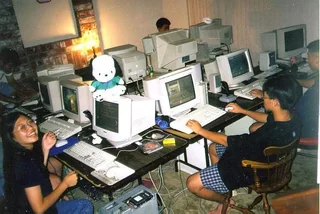
\includegraphics[width=1\linewidth]{images/quakelan.png}
    \caption{LAN party in the late 1990s—a grassroots precursor to modern esports.}
    \label{fig:lanparty}
\end{figure}

The rise of online gaming redefined digital entertainment as a structured and competitive experience. The introduction of \textbf{matchmaking systems}, \textbf{ranking ladders}, and \textbf{persistent progression mechanics} transformed casual play into continuous skill-based challenges. Pioneering titles such as \textbf{Quake}, \textbf{Counter-Strike}, and \textbf{StarCraft} set the standard for modern competitive games, combining reflex-based gameplay with strategic depth.

These systems offered players clear feedback loops—performance metrics, leaderboards, win/loss ratios—that fueled their desire to improve and dominate. As a result, gaming began to evolve from a leisure activity into a compelling arena of personal achievement and social recognition.

\subsection{From Networks to Virtual Battlefields}

The transformation of video games into \textbf{virtual battlefields} was fueled by technological advancements, global connectivity, and the rise of online communities. With real-time multiplayer becoming the norm, players worldwide could compete instantly, honing tactics and strategies to achieve recognition.

Video games offered an ideal competitive environment: \textbf{clear rules}, \textbf{quantifiable performance}, and \textbf{equal access}. As participation expanded, so did the supporting infrastructure—grassroots tournaments evolved into professional leagues, and casual players into sponsored competitors.

This convergence of entertainment, technology, and sport gave rise to \textbf{esports}, a global industry with professional teams, media coverage, and multimillion-dollar prize pools. What began as leisure became a legitimate career path and a powerful cultural force.

The same instinct that once ensured survival now drives mastery in digital arenas, where \textbf{technical skill, cognitive agility}, and \textbf{strategic thinking} define success.

The next chapters examine how this competitive landscape has also fostered new forms of rule-breaking. We will explore the evolution of \textbf{cheating} as both a technical challenge and a cultural phenomenon, revealing how players manipulate systems designed to ensure fair play.

 \chapter{The Evolution of Cheating: From Debugging Tools to an Organized Industry}

The history of cheating in video games is deeply intertwined with the evolution of the industry itself. What began as debugging tools for developers gradually transformed into a clandestine culture of modifications, and with the advent of online gaming, an organized and profitable industry with ties to cybercrime \parencite{consalvo2007cheating}. At the same time, the fight against cheating led to the development of \textbf{anti-cheat systems}, which evolved from simple integrity checks to sophisticated solutions incorporating artificial intelligence and deep system access \parencite{yan2005cheats}.

\section{The Early Days: Debugging Tools and Experimental Modifications}

Before video games became a mainstream form of entertainment, early cheating emerged as a necessity within software development. In the 1970s and 1980s, developers embedded debugging tools within their games to facilitate testing. These systems allowed programmers to modify internal values such as lives, ammunition, and speed, enabling them to test different scenarios without playing through the entire game \parencite{smith2018konami}.

Some of these tools remained accessible in commercial releases, either unintentionally or as a deliberate choice by developers. This led to the creation of the first \textbf{cheat codes}, which were key combinations or commands that altered gameplay. One of the most iconic examples is the \textbf{Konami Code} (↑ ↑ ↓ ↓ ← → ← → B A), introduced in \textit{Gradius} (1986) and later popularized in \textit{Contra} (1988) \parencite{kent2001ultimate}. While these codes were not designed to affect competition, they set a precedent for the intentional modification of gameplay.

\section{The Rise of Cheating in Consoles and PC}

As the video game industry grew throughout the 1980s and 1990s, cheating expanded beyond debugging tools and built-in cheat codes. With the advent of home consoles, external devices specifically designed to modify gameplay began to appear.

\subsection{Cheat Devices: Game Genie, GameShark, and Pro Action Replay}

The first dedicated cheat devices were \textbf{modification cartridges}, such as the \textbf{Game Genie} (1990) and the \textbf{GameShark} (1995). These hardware add-ons allowed players to inject custom modifications into a game’s memory, altering key parameters such as health, ammunition, and physics \parencite{supercade2001}. While initially marketed as harmless tools for enhancing single-player experiences, they introduced the concept of \textbf{real-time game manipulation}, which would later be adapted for online environments.

On the PC side, the introduction of \textbf{memory editors} provided users with a more flexible and powerful way to modify game values at runtime. Early programs like \textbf{Cheat Engine} (2000) enabled players to search for specific in-game variables and alter them directly, bypassing the limitations of built-in cheat codes \parencite{gamersatwork2012}. This shift from \textbf{developer-sanctioned cheats} to \textbf{unauthorized external modifications} laid the foundation for more advanced game-hacking techniques.

As gaming technology evolved, so did the tools available for modifying game memory structures. More sophisticated programs such as \textbf{ReClass.NET} emerged, allowing users to analyze and modify game memory at a structural level. Unlike traditional memory scanners, ReClass.NET enables users to reverse-engineer game memory layouts by dynamically inspecting class structures and data offsets in real time \parencite{wang2015reclass}. This advancement significantly improved the ability of cheat developers to create complex modifications, ranging from automatic aimbots to more intricate exploits that manipulate how game logic processes data.

\begin{figure}[h!]
    \centering
    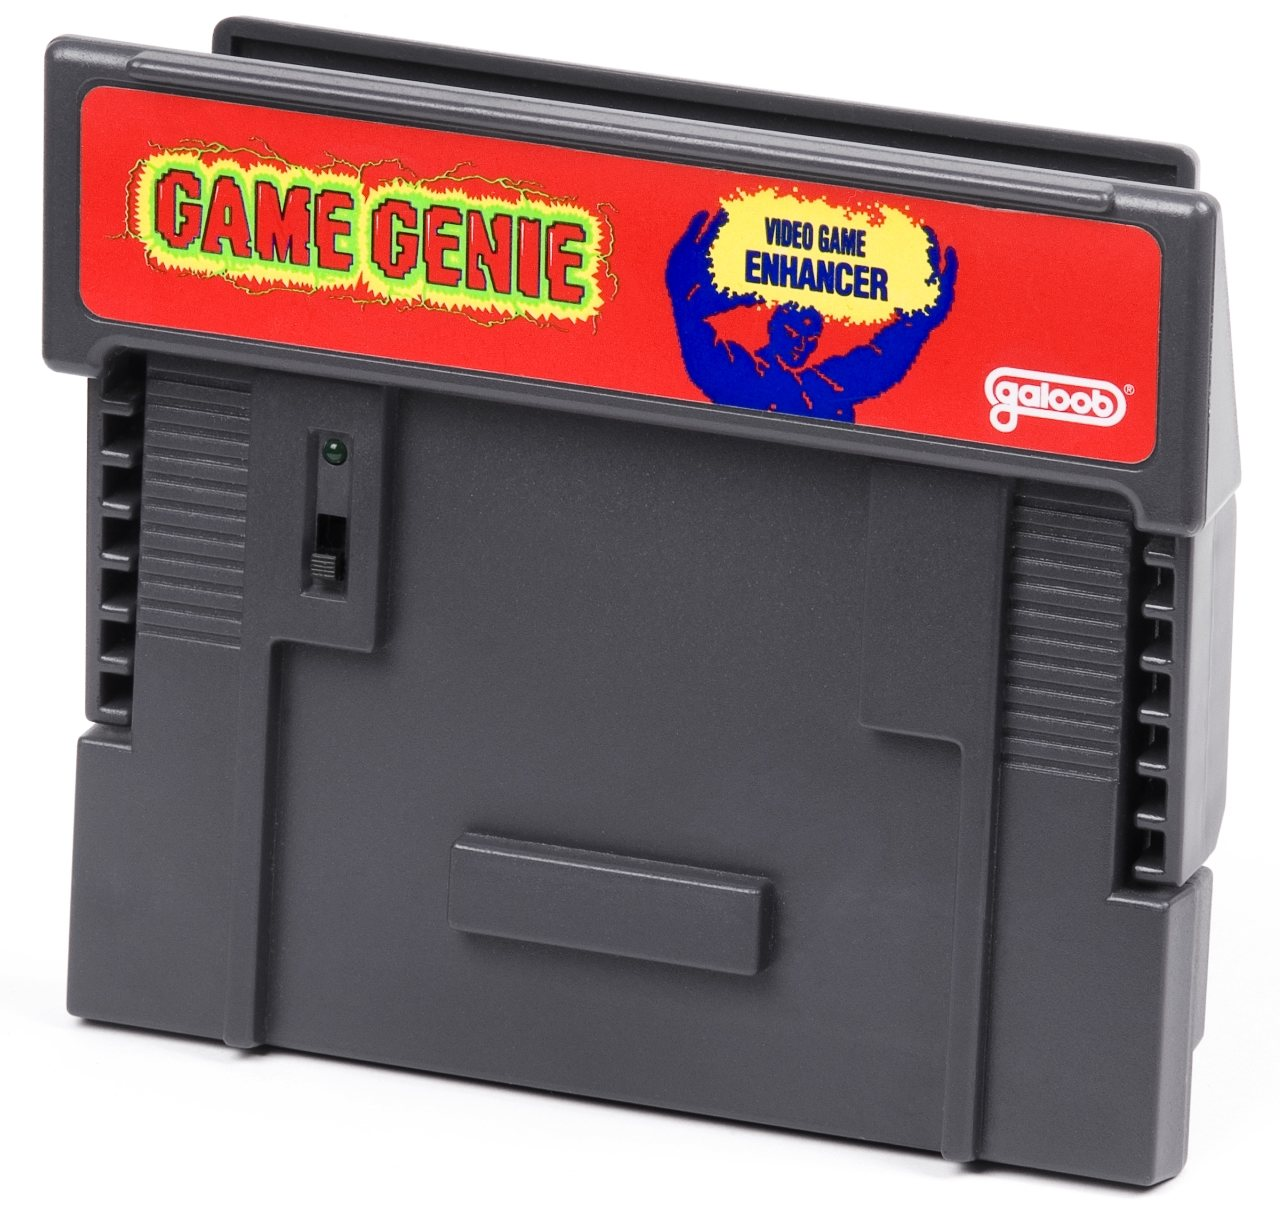
\includegraphics[width=0.5\linewidth]{images/logo-12.jpg}
    \caption{Game Genie}
    \label{fig:enter-label}
\end{figure}

\newpage
These tools, originally designed for educational and debugging purposes, soon became widely used in cheat development, particularly in online gaming environments. As their complexity increased, anti-cheat systems had to adapt rapidly, resulting in an ongoing technological competition between cheat developers and security teams.

\section{The Transition to Online Gaming: Cheating Becomes a Competitive Threat}

The rise of online multiplayer gaming in the late 1990s and early 2000s fundamentally changed the impact of cheating. Unlike single-player cheats, which only affected the individual experience, online cheating directly disrupted fair competition \parencite{yan2005cheats}. As games like \textbf{Quake} (1996), \textbf{Counter-Strike} (1999), and \textbf{Diablo II} (2000) introduced matchmaking and ranking systems, the incentive to cheat increased dramatically \parencite{young2016history}.

As competitive integrity gained prominence, developers began to implement more aggressive measures against cheating, resulting in the creation of server-side and client-side anti-cheat mechanisms. However, as anti-cheat solutions became more sophisticated, cheating techniques also advanced, producing a continuous cycle of adaptation between game security teams and cheat developers.

This progression led to the development of the first organized cheat communities, where players and programmers shared exploits, scripts, and modified game clients. It also marked the beginning of a persistent competition between cheat developers and game security teams, as new forms of cheating emerged alongside increasingly complex anti-cheat measures.

\section{The Birth and Evolution of Anti-Cheat Systems}

As online gaming became increasingly competitive, the integrity of fair play was challenged by the widespread use of cheats. Unlike single-player modifications, which had no broader consequences, cheating in multiplayer environments compromised \textbf{matchmaking, rankings, and esports competitions}, creating frustration among players and damaging the credibility of competitive gaming. 

Early attempts to mitigate cheating relied on \textbf{server-side validation}, where game servers monitored player actions for anomalies that suggested external manipulation. These checks aimed to detect unnatural behavior, such as \textbf{impossible movement speeds, improbable accuracy, and modifications to game assets} that altered visibility constraints. However, this approach had significant limitations, as many cheats operated entirely on the \textbf{client side}, modifying game data before it was transmitted to the server. As a result, more sophisticated \textbf{client-side anti-cheat solutions} were developed to monitor and detect unauthorized modifications directly within the player’s system.

One of the first dedicated anti-cheat programs was \textbf{PunkBuster}, developed by Even Balance, Inc. and introduced in \textbf{2000}. Initially implemented in \textit{Return to Castle Wolfenstein} and later in \textit{Battlefield 1942}, PunkBuster marked a shift from basic server-side detection to \textbf{active client-side monitoring}. It worked by scanning a player’s system for \textbf{known cheat signatures}, verifying \textbf{game file integrity}, and capturing periodic \textbf{in-game screenshots} to identify visual modifications such as \textbf{wallhacks}. Additionally, PunkBuster maintained a \textbf{global ban list}, preventing known cheaters from accessing protected servers. Despite these advancements, \textbf{cheat developers quickly adapted} by employing techniques such as \textbf{code obfuscation}, allowing their software to remain undetected. PunkBuster also faced criticism for its \textbf{aggressive scanning approach}, which occasionally resulted in \textbf{false positives}, banning legitimate players due to conflicts with background applications.

In \textbf{2002}, Valve introduced \textbf{Valve Anti-Cheat (VAC)} alongside \textit{Counter-Strike 1.6}, implementing a more \textbf{automated and data-driven approach} to cheat detection. Unlike PunkBuster, which \textbf{immediately expelled} suspected cheaters, VAC introduced a \textbf{delayed banning system}. This strategy allowed suspected cheaters to continue playing while logging their infractions, making it harder for cheat developers to \textbf{identify detection triggers} and modify their cheats accordingly. In addition to \textbf{signature-based detection}, VAC utilized \textbf{heuristic analysis} to recognize \textbf{abnormal behavioral patterns}, refining its detection algorithms over time. By integrating \textbf{server-side validation} with \textbf{machine learning techniques}, VAC continuously improved its ability to detect and counteract evolving cheats. However, since it \textbf{operated at the user level} rather than the \textbf{kernel level}, advanced cheats that manipulated system memory with higher privileges could still \textbf{bypass its protections}.

As cheat developers refined their evasion techniques, more aggressive anti-cheat solutions emerged. One of the most notable advancements was \textbf{BattleEye}, introduced in 2004 and later adopted in games such as \textit{Arma 2}, \textit{Rainbow Six Siege}, and \textit{PUBG}. Unlike VAC, which prioritized passive detection, BattleEye enforced stricter security measures by running with elevated system privileges. By operating at the kernel level, it could detect and block cheat software that manipulated game memory at a deeper level, making it significantly harder for external programs to alter in-game data without detection. This approach enabled BattleEye to intercept and prevent unauthorized modifications before they could affect gameplay, providing a more proactive defense against sophisticated cheats.

As competitive gaming and esports continued to grow, Riot Games introduced a new anti-cheat solution, Vanguard, designed specifically for \textit{Valorant}. Released in 2020, Vanguard elevated anti-cheat enforcement by implementing persistent kernel-level monitoring. This system actively runs as a background process from the moment the operating system starts, enabling it to detect and prevent unauthorized modifications at the lowest levels of system memory. While this approach is one of the most invasive and effective anti-cheat solutions, its intrusive nature sparked controversy among players concerned about privacy, as the software maintains continuous access to system processes even when the game is not running.

The evolution of anti-cheat systems reflects a continuous technological competition between cheat developers and game security teams. While early efforts relied on rudimentary server-side validation, modern solutions integrate behavioral analysis, machine learning, and kernel-level access to provide more robust protection. Despite these advancements, cheat developers continually adapt, ensuring that no anti-cheat system remains impenetrable for long. This dynamic perpetuates an ongoing cycle of exploitation and countermeasures in the digital landscape of competitive gaming.

This historical evolution has given rise to a wide variety of anti-cheat implementations, each shaped by the needs and challenges of its era.

The continuous development of anti-cheat solutions over the past two decades can be summarized through a timeline of key technologies. Figure~\ref{fig:timeline-anticheat-balanced} provides a chronological overview of the most influential anti-cheat systems, from early client-side detectors to modern kernel-level and behavior-based solutions.

\begin{figure}[h!]
    \centering
    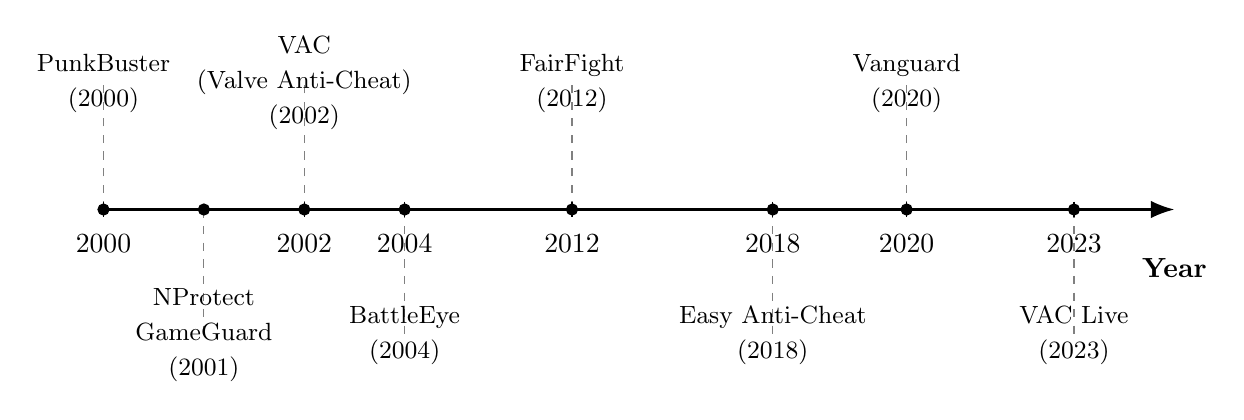
\begin{tikzpicture}[x=0.85cm, y=1cm]
        % Línea del tiempo
        \draw[thick, -{Latex[length=3mm]}] (0,0) -- (16,0);
        \node[below=0.5cm] at (16,0) {\textbf{Year}};

        % Eventos ajustados manualmente (x ≠ año directamente)
        \foreach \x/\year/\label/\ypos in {
            0/2000/PunkBuster/1.6,
            1.5/2001/NProtect\\GameGuard/-1.6,
            3/2002/VAC\\(Valve Anti-Cheat)/1.6,
            4.5/2004/BattleEye/-1.6,
            7/2012/FairFight/1.6,
            10/2018/Easy Anti-Cheat/-1.6,
            12/2020/Vanguard/1.6,
            14.5/2023/VAC Live/-1.6
        } {
            \draw[gray, dashed] (\x,0) -- (\x,\ypos);
            \filldraw[black] (\x,0) circle (2pt);
            \node[align=center, font=\small] at (\x,\ypos) {\label\\(\year)};
        }

        % Marcas de tiempo estilizadas
        \foreach \x/\label in {
            0/2000, 3/2002, 4.5/2004, 7/2012,
            10/2018, 12/2020, 14.5/2023
        } {
            \draw (\x,0.1) -- (\x,-0.1);
            \node[below] at (\x,-0.2) {\label};
        }

    \end{tikzpicture}
    \caption{Chronological overview of key anti-cheat systems introduced between 2000 and 2023.}
    \label{fig:timeline-anticheat-balanced}
\end{figure}

Among the systems depicted in the timeline, several stand out for their unique approach and impact.

nProtect GameGuard, launched in 2001, was among the first anti-cheat solutions to employ rootkit-like behavior. Widely used in Asian MMORPGs, it integrates deeply into the operating system, operating at the kernel level (ring 0), to prevent cheats from interacting with game processes. This deep integration has raised concerns about privacy and system stability \parencite{nprotect_wikipedia}.

FairFight, introduced in 2012, departed from traditional detection mechanisms by using server-side statistical analysis to flag abnormal player behavior. Instead of inspecting memory or processes, it relied on gameplay metrics such as accuracy, reaction time, and movement patterns. This approach made it less intrusive, but also vulnerable to both false positives and high-skill players \parencite{fairfight_website}.

Easy Anti-Cheat (EAC), which gained traction in 2018, became a popular choice for fast-paced competitive games. It combines kernel-level access with performance-friendly design and supports real-time detection of unauthorized drivers, injected DLLs, and tampering attempts, balancing robustness and user transparency \parencite{eac_website}.

Finally, VAC Live, unveiled in 2023, represents Valve's shift toward real-time, data-driven cheat prevention. Unlike the original VAC system, which relied on delayed bans, VAC Live is designed to detect and react to cheats during gameplay. This makes it a critical component in safeguarding the integrity of high-stakes esports matches \parencite{vac_live_announcement}.


\section{The Commercialization of Cheating}

The commercialization of video game cheating has evolved into a multifaceted ecosystem encompassing knowledge-sharing communities, grey-market resellers, and professionalized cheat providers. This transformation reflects a shift from informal exchanges to structured operations with varying degrees of legality and ethical considerations.

Platforms such as \textbf{UnKnoWnCheaTs} serve as non-commercial forums dedicated to the dissemination of information related to game hacking. These communities focus on educational content, including reverse engineering tutorials, memory manipulation techniques, and the release of free cheats contributed by community members. Notably, UnKnoWnCheaTs maintains a strict policy against the sale of cheats, emphasizing its commitment to a non-profit model centered on knowledge exchange \parencite{unknowncheats_forum}.

In contrast, forums like \textbf{ElitePVPers} and \textbf{MPGH} operate as marketplaces where individuals can buy and sell cheats. These platforms facilitate the distribution of paid cheats through various models, including reselling arrangements and subscription-based access. Users often engage in discussions about becoming resellers, highlighting the existence of structured networks for cheat distribution \parencite{elitepvpers_reseller}.

Beyond community forums, a segment of the cheating industry comprises professionalized providers offering sophisticated cheat solutions. These entities develop and sell advanced cheating tools, often featuring capabilities such as kernel-level access, hardware ID spoofing, and real-time updates to circumvent anti-cheat measures. The following table summarizes prominent cheat providers active in the CS2 ecosystem:

\newpage

\begin{table}[h!]
    \centering
    \renewcommand{\arraystretch}{1.4}
    \begin{tabular}{|p{3.2cm}|c|p{4cm}|p{3.8cm}|}
        \hline
        \textbf{Provider} & \textbf{Released} & \textbf{Subscription Price} & \textbf{Access Model} \\
        \hline
        \textbf{Neverlose} \parencite{neverlose2020} & 2020 & €29/month, €69/3 months, €129/year & Invite-only \\
        \hline
        \textbf{Memesense} \parencite{memesense2023} & 2023 & \$4/14 days, \$8/month, \$12/3 months & Public access \\
        \hline
        \textbf{Fatality.win} \parencite{fatality2022} & 2022 & \$33/month & Invite-only \\
        \hline
        \textbf{Project Infinity} \parencite{projectinfinity2017} & 2017 & €14.99/month, €29.99/3 months, €99.99 lifetime & Public access \\
        \hline
        \textbf{Midnight} \parencite{midnight2019} & 2019 & £5.15/month & Public access \\
        \hline
        \textbf{Onetap} \parencite{onetap2024} & 2024 & \$20/month & Public access \\
        \hline
        \textbf{Skeet (Gamesense)} \parencite{skeet2016} & 2016 & \$20/month & Invite-only + HWID locked \\
        \hline
    \end{tabular}
    \caption{Overview of major CS2 cheat providers, including release year, pricing models, and access restrictions.}
    \label{tab:cs2_cheat_providers}
\end{table}


\section*{From Historical Context to Market Impact}

Having explored the historical and sociotechnical evolution of video game cheating, from its inception with debugging tools to its current status as a sophisticated and commercialized industry, we now shift our focus to contemporary market dynamics and their ramifications on gaming communities.

The subsequent chapters will examine the economic structures underpinning the cheating industry, analyzing how monetized cheating services influence player behavior, community trust, and the overall integrity of online gaming environments. Through this analysis, we aim to elucidate the broader social and economic impacts of cheating within the gaming ecosystem.

With the historical framework established, we now proceed to assess the market-driven aspects that perpetuate and shape the landscape of video game cheating.
\newpage




 \chapter{The Prevalence and Impact of Cheating in Online Multiplayer Games}

Building upon the historical and sociotechnical evolution of video game cheating, from its origins in debugging tools to its current manifestation as a sophisticated, commercialized industry, we now examine its pervasive impact on contemporary gaming communities and market dynamics.

Cheating in online multiplayer games constitutes an escalating systemic threat that undermines fairness, erodes player trust, and destabilizes gaming ecosystems. This chapter delves into the multifaceted consequences of cheating, with particular emphasis on the evolving landscape surrounding \textit{Counter-Strike 2} (CS2), and argues that addressing this issue demands an integrated response encompassing technical, legal, and social countermeasures.

As competitive online titles continue to thrive, especially those featuring ranked ladders, esports ecosystems, and in-game economies, the incentives to obtain unfair advantages intensify. This dynamic perpetuates a relentless arms race between cheat developers and game studios, necessitating not only robust technological defenses but also a comprehensive understanding of the socio-economic impacts of cheating.

\section{Cheating as a Critical Threat to Player Retention}

Cheating is not merely a minor inconvenience; it stands as a significant factor contributing to player attrition and dissatisfaction. A global survey conducted by Irdeto revealed that 60\% of players reported a negative impact on their gaming experience due to cheating, and 77\% indicated they would discontinue playing a game if cheating became widespread \parencite{irdeto2018global}.

\begin{table}[H]
  \centering
  \caption{Survey Results on Cheating in Online Games (Irdeto, 2018)}
  \label{tab:irdeto-survey}
  \begin{tabular}{|p{10cm}|c|}
  \hline
  \textbf{Survey Statement} & \textbf{Percentage of Respondents} \\
  \hline
  Experienced negative impact due to cheating & 60\% \\
  Would stop playing a game because of cheaters & 77\% \\
  Support permanent bans for cheaters & 69\% \\
  Believe developers are not doing enough & 55\% \\
  \hline
  \end{tabular}
\end{table}

These findings underscore that cheating not only generates immediate frustration but also carries long-term economic implications. Since player engagement drives monetization through mechanisms such as battle passes, cosmetic sales, and advertising, a decline in player retention fueled by cheating poses a direct threat to publishers' revenue streams.

Ultimately, when players perceive ranked systems, matchmaking, or competitive outcomes as compromised, they are likely to migrate toward alternative titles, thereby undermining the sustainability and vitality of the gaming community.

\section{Case Study: Cheating in \textit{Counter-Strike 2}}

\textit{Counter-Strike 2} (CS2) stands as a prominent example of modern cheating dynamics within competitive first-person shooter games. Its expansive player base and vibrant esports scene make it both an attractive target for cheat developers and a critical testing ground for anti-cheat innovations.

To contextualize the scale of CS2's ecosystem, Figure~\ref{fig:cs2-playerbase} illustrates the evolution of its player base from January 2024 to April 2025, based on data from SteamCharts:

\begin{figure}[H]
  \centering
  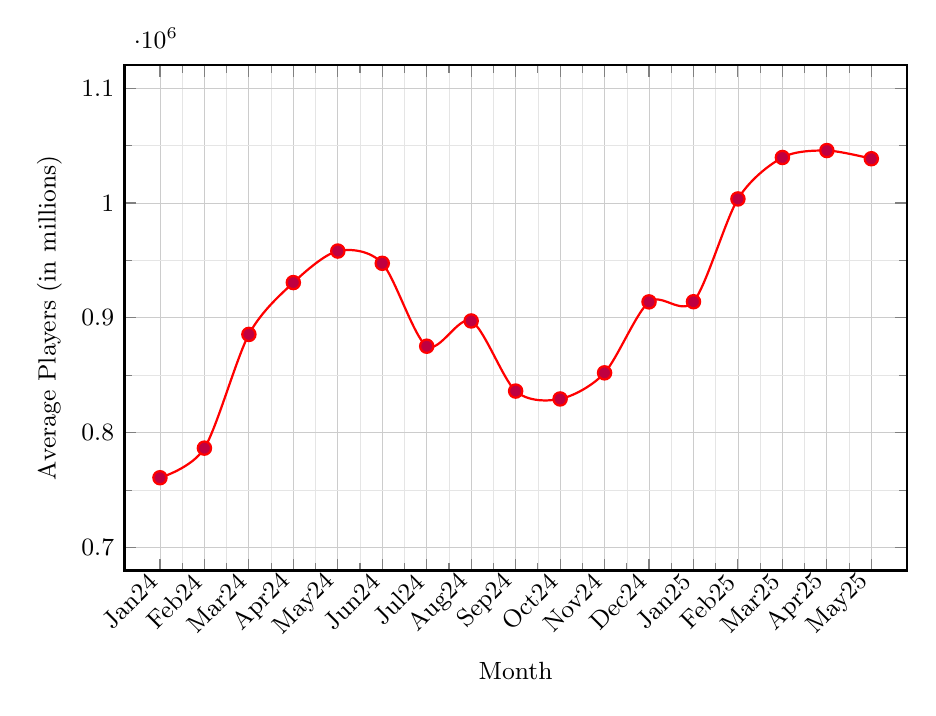
\begin{tikzpicture}
  \begin{axis}[
      width=0.95\textwidth,
      height=8cm,
      xlabel={Month},
      ylabel={Average Players (in millions)},
      symbolic x coords={Jan24, Feb24, Mar24, Apr24, May24, Jun24, Jul24, Aug24, Sep24, Oct24, Nov24, Dec24, Jan25, Feb25, Mar25, Apr25, May25},
      xtick=data,
      xticklabel style={rotate=45, anchor=east, font=\small},
      yticklabel style={font=\small},
      label style={font=\small},
      tick style={thin},
      grid=both,
      minor tick num=1,
      major grid style={line width=.3pt, draw=gray!40},
      minor grid style={line width=.2pt, draw=gray!20},
      ymin=700000, ymax=1100000,
      enlargelimits=0.05,
      smooth,
      mark options={scale=1.2, fill=purple!100},
      line width=0.8pt,
  ]
  \addplot[
      color=red,
      mark=*,
  ]
  coordinates {
      (Jan24,760859) (Feb24,786631) (Mar24,885630) (Apr24,930749)
      (May24,958207) (Jun24,947521) (Jul24,875365) (Aug24,897338)
      (Sep24,836307) (Oct24,829439) (Nov24,852164) (Dec24,913953)
      (Jan25,914092) (Feb25,1003571) (Mar25,1039663) (Apr25,1045702)
      (May25,1038597)
  };
  \end{axis}
  \end{tikzpicture}
  \caption{Evolution of Average CS2 Player Counts (January 2024 to May 2025). Source: SteamCharts.}
  \label{fig:cs2-playerbase}
\end{figure}

The consistent growth in CS2's player base underscores the game's enduring popularity and its pivotal role in the competitive FPS landscape. However, this expansion introduces increased complexity; a larger and more diverse player community amplifies the challenges associated with maintaining competitive integrity.

\newpage

Data from recent enforcement activities further highlights the scale and persistence of the issue \parencite{csstats2024}:

\begin{table}[H]
  \centering
  \small
  \setlength{\tabcolsep}{6pt}
  \caption{Activity of Banned Accounts Prior to Enforcement (January to April 2024)}
  \label{tab:cheater-impact}
  \begin{tabular}{|p{5.2cm}|c|}
  \hline
  \textbf{Metric} & \textbf{Estimated Value} \\
  \hline
  Average delay between last match and VAC ban & 20 days \\
  \hline
  Percentage of bans issued within 24 hours & 28\% \\
  \hline
  Total matches played by banned accounts & Over 32,000 \\
  \hline
  Percentage of matches with only one banned player & 97\% \\
  \hline
  Evidence of case farming behavior & Not significant \\
  \hline
  \end{tabular}
\end{table}

These observations reveal that cheaters are not isolated anomalies; rather, they are embedded within regular matchmaking sessions, further complicating detection and enforcement efforts.

\subsection{Trust Factor and Reporting System Limitations}

To mitigate cheating and enhance matchmaking quality, Valve implemented the \textit{Trust Factor} system in \textit{Counter-Strike 2} (CS2).

\begin{tcolorbox}[colback=gray!10, colframe=gray!50, boxrule=0pt, sharp corners, width=\linewidth, left=1mm, right=1mm, top=0.5mm, bottom=0.5mm]
\makebox[\linewidth][c]{\textbf{Definition: Trust Factor Explained}} \\
The Trust Factor system aggregates multiple indicators such as VAC bans, player reports, account age, and Steam community standing to adjust matchmaking quality. Its opacity aims to prevent manipulation but can lead to confusion and potential exploitation.
\end{tcolorbox}

While the Trust Factor system provides a foundation for fair matchmaking, its lack of transparency presents two significant challenges: (1) players have limited means to understand or improve their Trust Factor; and (2) third-party services offering \textit{report bots} and \textit{commend bots} can manipulate trust metrics for profit \parencite{cs2trustfactor2024}.

\subsection{Economic and Psychological Impact}

The ramifications of cheating extend beyond gameplay, inflicting substantial economic and psychological harm. In early 2025, a significant VAC enforcement wave resulted in the permanent banning of accounts with inventories collectively valued at approximately \$2 million \parencite{escorenews2025vacban}. Although this action was lauded as a crackdown on cheaters, it also raised concerns about transparency and the potential for false positives.

\begin{tcolorbox}[colback=gray!10, colframe=gray!50, boxrule=0pt, sharp corners, width=\linewidth, left=1mm, right=1mm, top=0.5mm, bottom=0.5mm]
\makebox[\linewidth][c]{\textbf{Definition: VAC Ban}} \\
A Valve Anti-Cheat (VAC) ban is a permanent restriction imposed when cheating activity is detected. It disables multiplayer functionality and trading privileges associated with the affected title.
\end{tcolorbox}

For players who have invested considerable time, resources, and personal attachment into their accounts, the psychological toll of encountering cheaters or being wrongfully penalized can be profound, leading to disengagement and a decline in community loyalty.

\section{Community Perception and the Culture of Cynicism}

Cheating incidents are highly visible across social platforms such as Reddit, YouTube, and Twitch. High-profile streamers encountering cheaters during broadcasts exacerbate perceptions of widespread dishonesty, even when empirical cheating rates remain relatively low.

This feedback loop fosters a culture of cynicism, where player trust in matchmaking systems and anti-cheat technologies diminishes, ultimately endangering long-term community stability.

\section{Legal and Ethical Responses to Cheat Development}

Recognizing the limitations of technical interventions, game developers have increasingly turned to legal avenues to combat cheat creators. A notable example is Bungie's legal action against Mihai Claudiu-Florentin, the operator of VeteranCheats, which resulted in a default judgment awarding Bungie \textbf{\$12,059,912.98} in damages. This amount encompassed statutory damages under the Digital Millennium Copyright Act (DMCA), actual damages for copyright infringement, and attorneys' fees and costs \parencite{torrentfreak2023bungie}.

This legal precedent has encouraged other companies, such as Riot Games, Ubisoft, and Activision, to adopt similar strategies in protecting their intellectual property and maintaining fair play within their gaming communities.

\newpage
\section{Anti-Cheat Technologies: Current Trends and Limitations}

Despite significant advancements, contemporary anti-cheat technologies predominantly operate in a reactive capacity, often lagging behind the evolving tactics of cheat developers.

Valve's \textit{Valve Anti-Cheat} (VAC) system primarily employs signature-based detection methods, scanning for known cheat signatures within the game's memory. This approach renders VAC susceptible to evasion techniques such as code obfuscation and manual mapping, which can bypass signature recognition mechanisms \parencite{turn0search0}.

Conversely, Riot Games' \textit{Vanguard} system adopts a more intrusive strategy by operating at the kernel level, granting it deep access to system processes. While this enhances its capability to detect sophisticated cheats, it has raised substantial privacy and security concerns among users due to its persistent presence and high-level system access \parencite{turn0search1}.

Emerging methodologies, including AI-driven behavioral analysis and the utilization of secure enclave technologies, present promising avenues for proactive cheat detection. AI-based systems can analyze player behavior in real-time to identify anomalies indicative of cheating, while secure enclaves offer isolated environments that protect sensitive computations from tampering. However, these approaches introduce new challenges, such as the potential for false positives and concerns regarding user data privacy \parencite{turn0search5, turn0search2}.

The ongoing battle between cheat developers and anti-cheat engineers constitutes a dynamic and relentless arms race, necessitating continuous innovation and adaptation to preserve the integrity of competitive gaming environments.

\vspace{1em}

\begin{tcolorbox}[colback=gray!10, colframe=gray!50, boxrule=0pt, sharp corners, width=\linewidth, left=1mm, right=1mm, top=0.5mm, bottom=0.5mm]
\textbf{Key Takeaways:}
\begin{itemize}
    \item Cheating poses a direct threat to player retention, game reputation, and revenue streams.
    \item Systems like \textit{Trust Factor} require increased transparency and user engagement to be effective.
    \item Legal actions are a critical component in combating organized cheat development and distribution.
    \item The fight against cheating is an ongoing, adaptive arms race necessitating continual technological and strategic innovation.
\end{itemize}
\end{tcolorbox}

 \chapter{Injection and Detection Techniques}

\section{Why Injection Matters in Cheat Development}

In professional game cheating, especially in competitive games like \textit{Counter-Strike 2}, most serious cheats are built as \textbf{DLLs} that are injected into the game's running process.

\begin{tcolorbox}[colback=gray!10, colframe=gray!10, boxrule=0pt, sharp corners, width=\linewidth, left=1mm, right=1mm, top=0.5mm, bottom=0.5mm]
\textbf{What is a DLL?} \\
A DLL (Dynamic Link Library) is like a small add-on that can be loaded into a program to extend what it can do. In the case of cheats, a DLL gives direct access to the game's memory and functions.
\end{tcolorbox}

Injecting a DLL allows the cheat to run \textbf{at the same time} as the game itself. This enables cheats to:

\begin{itemize}
    \item \textbf{Hook game functions} to change behavior (e.g., aiming or vision systems).
    \item \textbf{Modify memory} to adjust gameplay (e.g., speed, ammo, recoil).
    \item \textbf{Read internal data} like player positions or weapon stats.
    \item \textbf{Draw overlays} directly on the screen (e.g., radar, ESP).
    \item \textbf{Automate actions} to perform tasks faster or more accurately.
\end{itemize}

Because of this deep integration, cheat injection is the main focus of anti-cheat systems like \textbf{Valve Anti-Cheat (VAC)}.

\section{Overview of Code Injection Techniques}

\textbf{Code injection} means inserting new code into a running program. In cheat development, this usually means adding a DLL or custom code into the game's memory.

\subsection*{Traditional Methods}

Earlier cheats used simple Windows functions like:

\begin{itemize}
    \item \texttt{LoadLibrary}: Loads a DLL into another process.
    \item \texttt{CreateRemoteThread}: Starts a new thread inside another program.
\end{itemize}

These methods are now easy for anti-cheats to detect because they leave obvious traces.

\subsection*{Manual Mapping}

Today, cheats mostly use a method called \textbf{Manual Mapping}.

\begin{tcolorbox}[colback=gray!10, colframe=gray!10, boxrule=0pt, sharp corners, width=\linewidth, left=1mm, right=1mm, top=0.5mm, bottom=0.5mm]
\textbf{What is Manual Mapping?} \\
Manual Mapping is a way of loading a DLL manually into a program’s memory without using Windows' normal loading functions. This makes it much harder for anti-cheat systems to notice the injection.
\end{tcolorbox}

Manual Mapping avoids showing up in the list of loaded modules and can start execution in stealthy ways, such as by hijacking existing game threads.

\begin{figure}[H]
    \centering
    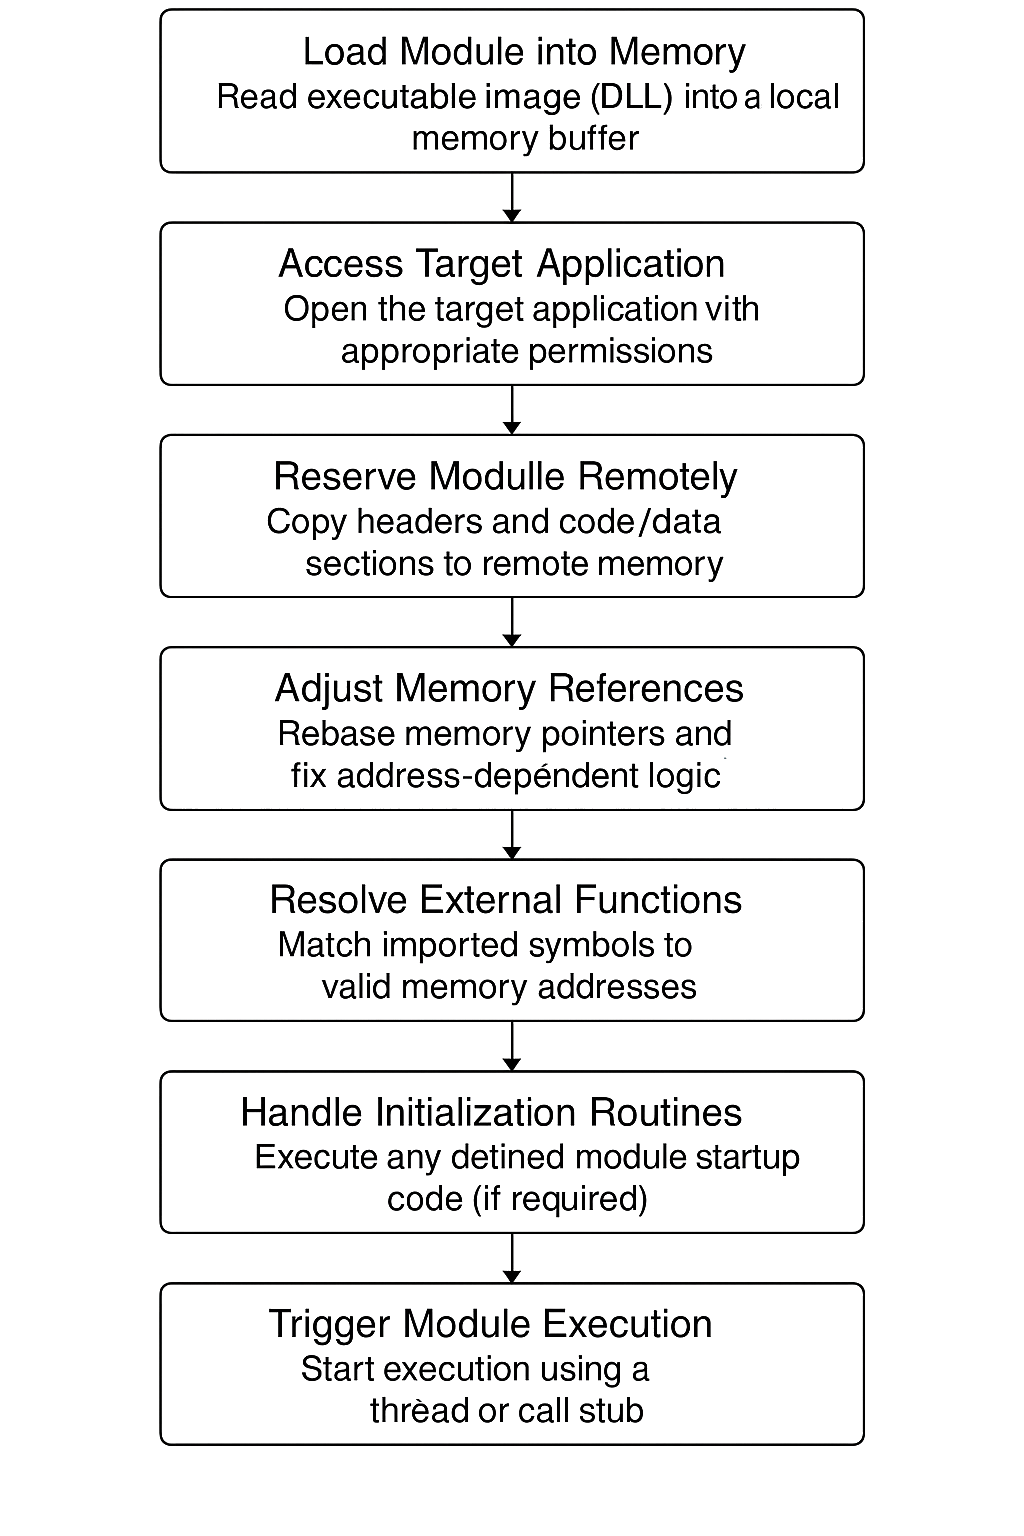
\includegraphics[width=0.60\textwidth]{images/diagram_white_background.png}
    \caption{Simplified flowchart of dynamic module injection using Manual Mapping.}
    \label{fig:manual_mapping_flow}
\end{figure}

We have developed our own injector that follows the structure outlined in Figure~\ref{fig:manual_mapping_flow}.  
The source code for this injector can be found in the \texttt{injector} branch of the project repository.

\section{Detection Techniques in Anti-Cheat Systems}

The detection techniques described in this section are \textbf{not merely theoretical}; they are the result of \textbf{practical reverse engineering} carried out on modules \textit{extracted (dumped)} directly from the game's memory during runtime.  
Through detailed analysis of the internal workings of \textbf{Valve Anti-Cheat (VAC)}, we have gathered \textbf{concrete evidence} supporting the mechanisms and strategies presented below.

Modern anti-cheat systems, such as VAC, deploy a wide range of methods to detect the presence of unauthorized code within game processes.  
These methods are specifically designed to identify \textit{abnormal memory modifications}, \textit{injected modules}, or \textit{manipulation of trusted system structures}.

In the following sections, we outline and explain the principal detection techniques observed during our research.

\subsection*{Thread Local Storage (TLS) Callbacks}

One early opportunity for anti-cheats to detect injected code occurs during program startup.  
When a program or DLL starts running, Windows can automatically execute special functions known as \textbf{TLS callbacks}.

\begin{tcolorbox}[colback=gray!10, colframe=gray!10, boxrule=0pt, sharp corners, width=\linewidth, left=1mm, right=1mm, top=0.5mm, bottom=0.5mm]
\textbf{What is a TLS Callback?} \\
A TLS (Thread Local Storage) callback is a special function that Windows automatically calls when a thread starts, before the main application code runs. Developers can use it for initialization tasks — but it can also be leveraged by anti-cheats for early memory inspections.
\end{tcolorbox}

Anti-cheats leverage this early execution stage to scan memory and inspect the runtime environment, often before the main game code even begins.

\begin{comment}
\begin{figure}[h!]
    \centering
        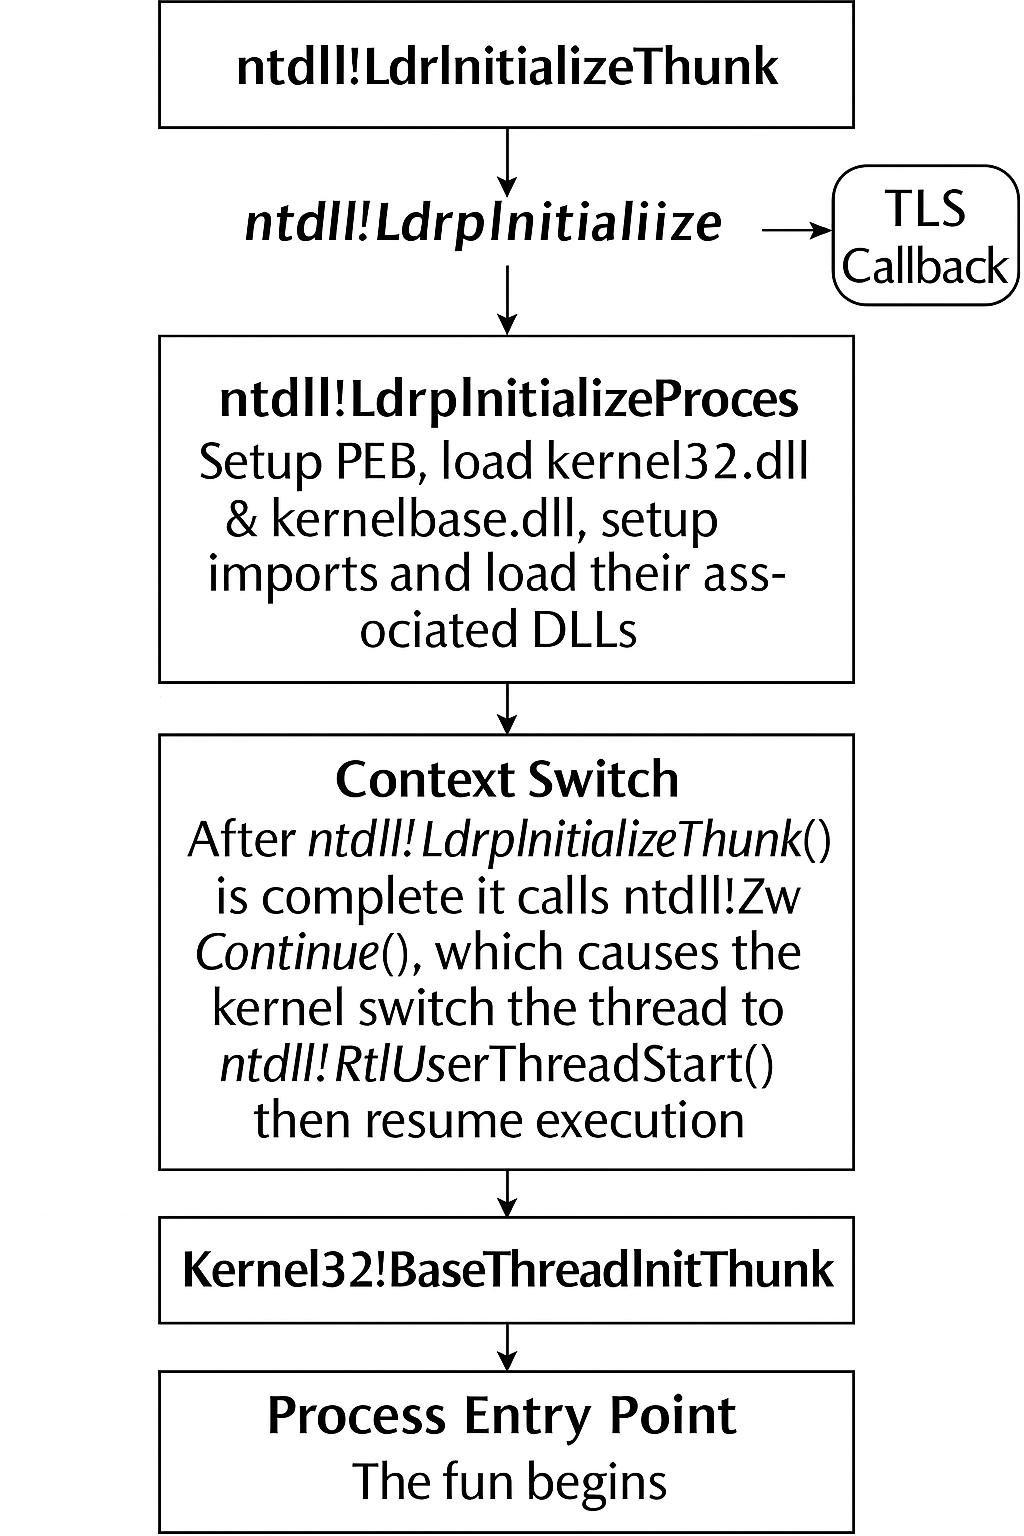
\includegraphics[width=0.45\textwidth]{images/tls_callback.png}
        \caption{Windows thread initialization with TLS Callback execution highlighted.}
        \label{fig:tls-callback-diagram}
\end{figure}
\end{comment}

If an injected DLL includes TLS callbacks and they are not properly removed or disabled, the cheat risks being detected immediately during process initialization.

\subsection*{Start Address Integrity Checks}

Beyond startup checks, anti-cheats like VAC continuously monitor thread creation during gameplay.  
A common detection method involves checking the \textbf{start address} of each thread.

\begin{tcolorbox}[colback=gray!10, colframe=gray!10, boxrule=0pt, sharp corners, width=\linewidth, left=1mm, right=1mm, top=0.5mm, bottom=0.5mm]
    \textbf{What is a Start Address?} \\
    The start address is the location in memory where a thread begins its execution. Legitimate threads typically start inside official game modules, such as \texttt{client.dll} or other trusted libraries.
\end{tcolorbox}    

If a thread is found starting at an address like \texttt{0x5F3A0000}, which falls outside any known game module (e.g., not within \texttt{client.dll}), it is highly suspicious and often indicates injected code or shellcode execution.

This method is particularly effective at catching poorly concealed code injections or shellcode execution.

\subsection*{VMT Hook Detection}

Another detection strategy focuses on the integrity of in-game objects.

In object-oriented engines, game entities typically use \textbf{Virtual Method Tables (VMTs)} to organize their functions.

\begin{tcolorbox}[colback=gray!10, colframe=gray!10, boxrule=0pt, sharp corners, width=\linewidth, left=1mm, right=1mm, top=0.5mm, bottom=0.5mm]
\textbf{What is a Virtual Method Table (VMT)?} \\
A VMT is a table used in object-oriented programming to map object methods to their actual function addresses. By modifying a VMT, an attacker can hijack how a game object behaves.
\end{tcolorbox}

Cheats often modify these tables to hijack behaviors, such as altering rendering or player input.

Anti-cheats like VAC can identify tampered VMTs by verifying:

\begin{itemize}
    \item Whether the VMT points to unexpected memory regions.
    \item Whether the methods referenced fall outside legitimate game or system modules.
\end{itemize}

\begin{figure}[h!]
    \centering
    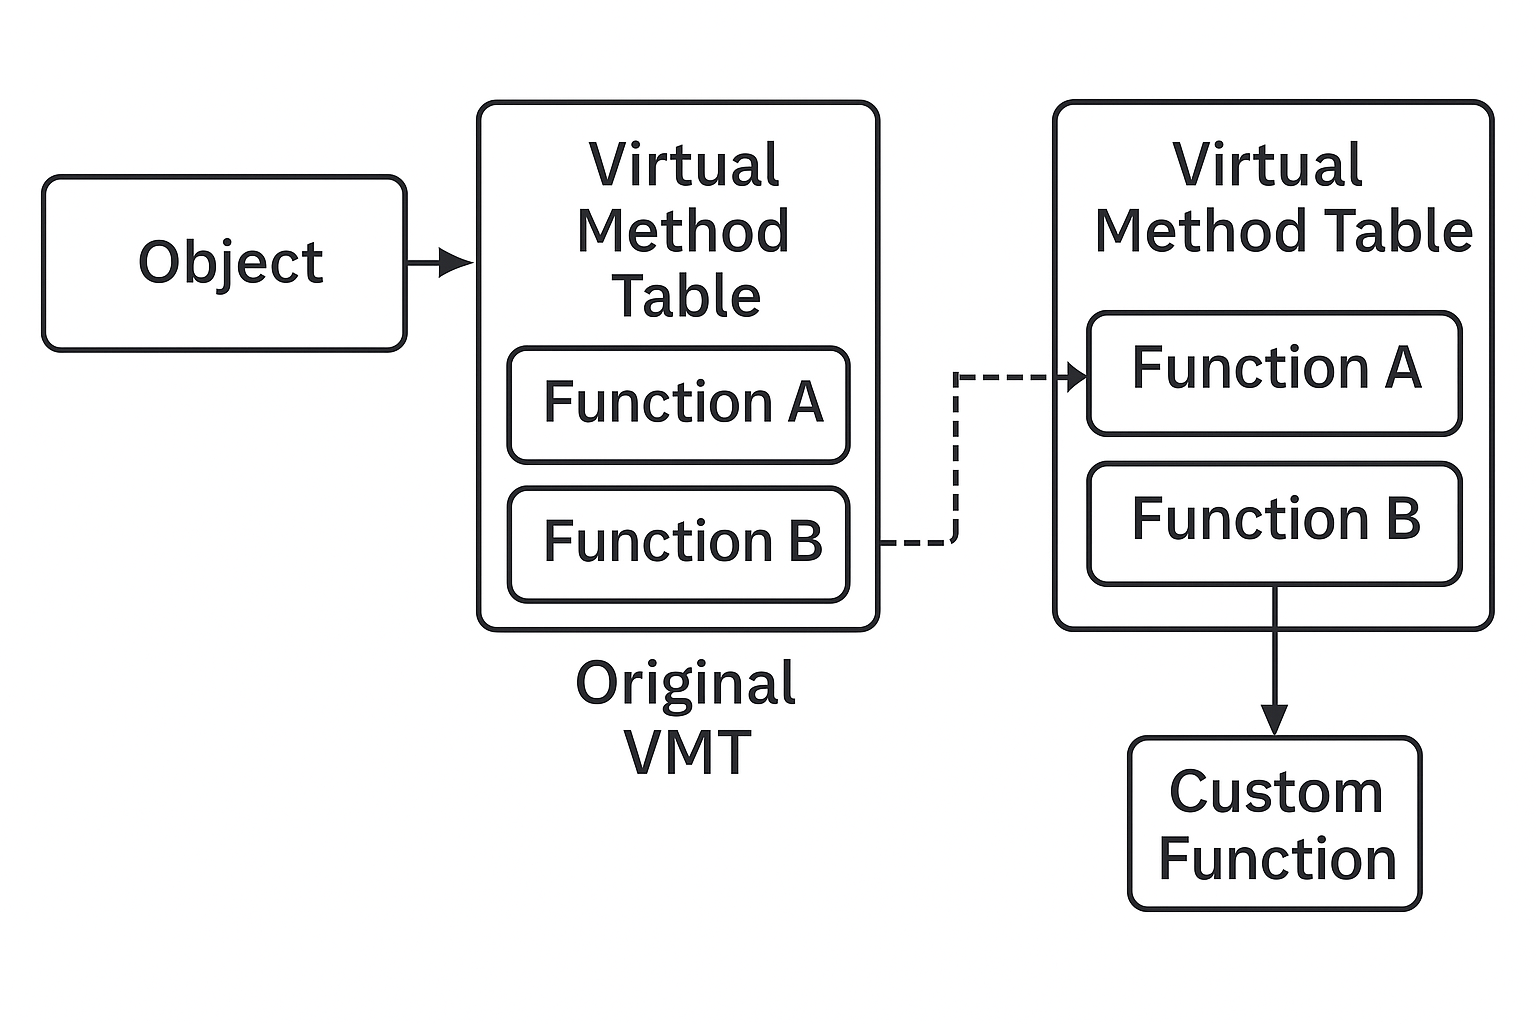
\includegraphics[width=0.65\textwidth]{images/vmthooking.png}
    \caption{Example of VMT Hooking.}
    \label{fig:vmt-hooking-diagram}
\end{figure}

Due to their clear memory footprint, traditional VMT hooks are now considered relatively high-risk in modern cheat development.

\section{Evasion Techniques Used by Cheats}

As anti-cheat systems like VAC become more sophisticated in their detection capabilities, cheat developers continuously adapt by designing increasingly advanced evasion techniques.  
These strategies aim to minimize the attack surface, avoid triggering heuristic scans, and maintain stealth even under active monitoring.

In this section, we present and explain some of the most common methods used to evade detection.


\subsection*{Suppressing TLS Callbacks}

To avoid early-stage detection, cheats often remove or disable the TLS callback directory from their injected DLLs.  
By doing so, they prevent anti-cheats from executing inspection routines before the cheat is fully concealed.

\subsection*{Thread Hijacking and Return Address Spoofing}

Instead of creating new threads—an action easily spotted—some cheats \textbf{hijack existing game threads}.

\begin{tcolorbox}[colback=gray!10, colframe=gray!10, boxrule=0pt, sharp corners, width=\linewidth, left=1mm, right=1mm, top=0.5mm, bottom=0.5mm]
\textbf{What is Thread Hijacking?} \\
Thread hijacking involves pausing an existing, legitimate thread, changing its instruction pointer to execute custom code, and then resuming it—making it harder for anti-cheats to notice any new activity.
\end{tcolorbox}

To further hide execution, cheats use \textbf{return address spoofing}—manipulating the call stack to make it appear that their code was naturally invoked from within the game’s legitimate modules.

\subsection*{Start Address Redirection via ROP Gadgets}

A more advanced and stealthy method used by cheats involves \textbf{Return-Oriented Programming (ROP)}.

\begin{tcolorbox}[colback=gray!10, colframe=gray!10, boxrule=0pt, sharp corners, width=\linewidth, left=1mm, right=1mm, top=0.5mm, bottom=0.5mm]
\textbf{What is a ROP Gadget?} \\
A ROP gadget is a small snippet of code already present in trusted modules, such as the game executable or Windows libraries. These snippets typically end with control transfer instructions like \texttt{ret} (return) or \texttt{jmp reg}.
\end{tcolorbox}

Instead of directly calling malicious code (which could be easily detected), cheats use ROP gadgets to build fake call chains.  
This way, their execution path appears legitimate, making detection much harder.

\paragraph{Stack Alignment and Shadow Space.}

In 64-bit Windows environments, the calling convention (\texttt{Microsoft x64}) imposes strict rules on how functions must be called, particularly regarding the stack layout:

\begin{itemize}
    \item \textbf{Stack Alignment}: Before calling any function, the stack pointer (\texttt{rsp}) must be 16-byte aligned. This ensures that SIMD instructions (like \texttt{movaps}) and internal ABI requirements function correctly.
    \item \textbf{Shadow Space}: Additionally, 32 bytes must be reserved on the stack for the called function to use freely. This space is used to store register parameters or local variables.
\end{itemize}

Failure to meet these requirements can cause functions to crash, corrupt data, or behave unpredictably.  
Moreover, violating calling conventions can raise suspicion in anti-cheat systems performing runtime integrity checks.

To correctly prepare the stack for a spoofed or redirected call during ROP, cheats must adjust the stack before jumping to the target function.

Here is an example of a minimal x64 call stub that correctly aligns the stack and reserves the required shadow space:

\begin{lstlisting}[style=asmstyle]
sub rsp, 0x28               ; reserve 32 bytes shadow space + align stack (16-byte alignment)
mov rax, 0xFFAAFFAAFFAAFFAA ; address of the ROP gadget to act as a fake return address
push rax                    ; push the fake return address onto the stack
mov rax, 0xFFAAFFAAFFAAFFAA ; address of the actual target function to execute
jmp rax                     ; jump to the real function
\end{lstlisting}

This setup ensures that:

\begin{itemize}
    \item The stack is properly aligned (after \texttt{sub rsp, 0x28}).
    \item A valid-looking return address (pointing to a trusted ROP gadget) is pushed.
    \item The function call structure looks legitimate, reducing the risk of detection.
\end{itemize}

Thus, when the called function finishes and executes a \texttt{ret} instruction, it returns to a safe, believable address instead of crashing or exposing the cheat.

\paragraph{Detection Vectors.}

While ROP techniques are highly stealthy, anti-cheats can still perform \textbf{stack walking}—analyzing the call stack at runtime to detect inconsistencies, fake return addresses, or suspicious memory regions.

\paragraph{Practical Implementations.}

Open-source projects like \texttt{x86RetSpoof} by danielkrupinski offer practical examples of return address spoofing.  
However, professional cheats often use customized ROP implementations tailored to specific games like CS2 for maximum stealth.

\section{Extended VAC Capabilities and Developer Countermeasures}

Beyond basic memory and thread inspections, \textbf{Valve Anti-Cheat (VAC)} extends its detection efforts through broader system monitoring.  
It actively scans the file system looking for known cheat artifacts, inspects running processes for suspicious memory regions or injected modules, monitors the Windows registry for abnormal entries, and tracks inter-process activity to detect unauthorized access to the game.

This expanded approach allows VAC to move beyond simple memory analysis, building a more complete picture of system behavior and making traditional static cheats easier to detect.

In response, cheat developers have introduced a range of countermeasures aimed at staying hidden.  
String encryption is commonly used to obfuscate identifiable patterns in memory. Name randomization changes module and window identifiers dynamically to avoid blacklists.  
More advanced techniques include polymorphic code, which mutates the cheat at runtime to evade pattern detection, and fileless execution, where the cheat operates entirely from memory without touching the disk.  
Memory cleansing after injection further minimizes visible traces that could expose the cheat during active scanning.

Ultimately, the ongoing battle between anti-cheat technologies and cheat developers drives constant innovation on both sides.  
As VAC strengthens its methods to detect unauthorized activity, cheats evolve to become more stealthy, adaptive, and resilient — ensuring that the arms race in competitive gaming security remains in constant motion.
%
 \chapter{Function Hooking and Trampoline-Based Interception}

\section*{Overview}

At the heart of our cheat framework lies a fundamental and widely-used technique: \textbf{function hooking}. This mechanism allows us to intercept and manipulate internal function calls within the game, modify their behavior, and seamlessly resume execution without disrupting the application’s control flow.

\begin{tcolorbox}[colback=gray!10, colframe=gray!10, boxrule=0pt, sharp corners, width=\linewidth, left=1mm, right=1mm, top=0.5mm, bottom=0.5mm]
\textbf{What is Function Hooking?} \\
Function hooking is the practice of redirecting a function’s execution flow to custom code. It enables the interception, modification, or extension of a program’s behavior without access to its source code.
\end{tcolorbox}

Among the various hooking strategies available, the most stable and stealthy is the \textbf{trampoline hook}.  
Trampoline hooking offers a reliable and elegant solution for redirecting code execution to custom payloads while preserving the original function’s logic.

In this chapter, we present an in-depth explanation of trampoline hooks—how they work, why they are effective, and how they can be implemented safely using the \texttt{MinHook} library.

\section{What is a Trampoline Hook?}

A trampoline hook works by overwriting the beginning of a target function with a jump (typically a near relative \texttt{JMP} or an absolute indirect jump) to a custom handler — our hook payload.  
Since this patch modifies the first few bytes of the original function, those instructions must first be preserved to avoid corrupting the original behavior.  
We do this by copying them into a new, executable memory region known as the \textit{trampoline}.

\begin{tcolorbox}[colback=gray!10, colframe=gray!10, boxrule=0pt, sharp corners, width=\linewidth, left=1mm, right=1mm, top=0.5mm, bottom=0.5mm]
\textbf{What is a Trampoline?} \\
A trampoline is a small section of executable memory that stores the original stolen instructions from a hooked function, allowing seamless continuation after custom code executes.
\end{tcolorbox}

Once our custom payload finishes, control passes to the trampoline, which executes the preserved instructions and then jumps back to the original function — resuming normal execution as if nothing had changed.

This redirection process involves four main components:

\begin{itemize}
  \item \textbf{Original (Hooked) Function}: The function entry point is patched to redirect execution.
  \item \textbf{Relay Function}: A lightweight stub that jumps to the hook payload.
  \item \textbf{Hook Payload}: Executes the desired cheat logic before invoking the trampoline.
  \item \textbf{Trampoline}: Holds the stolen instructions and redirects execution back into the original code.
\end{itemize}

\begin{figure}[H]
  \centering
  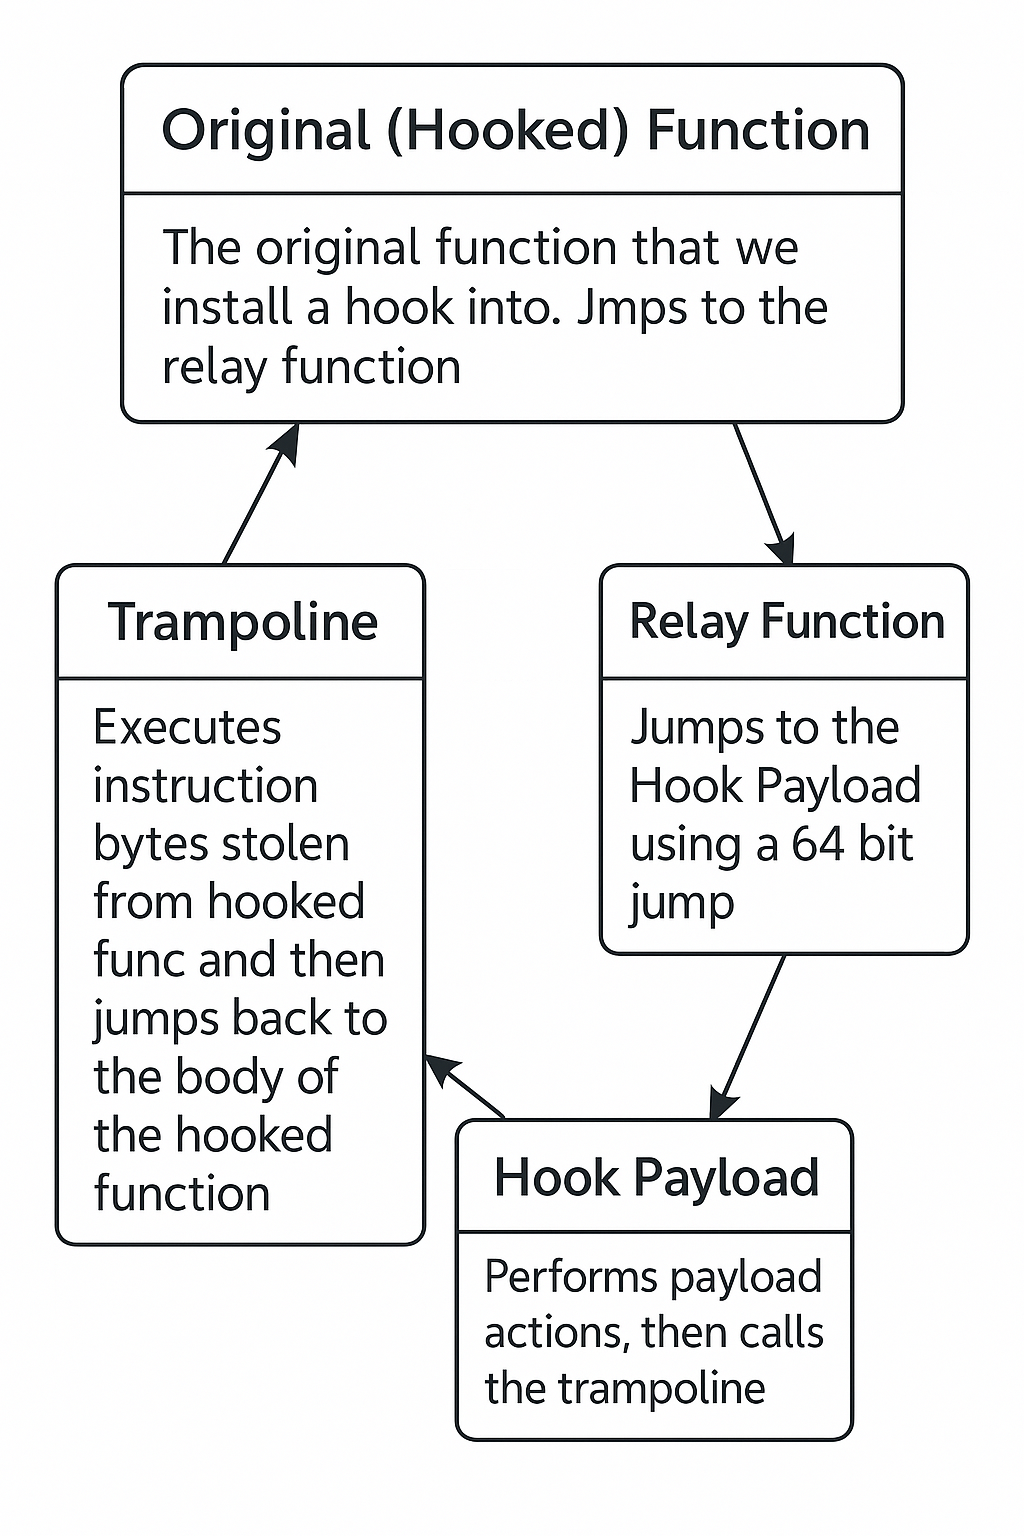
\includegraphics[width=0.55\textwidth]{images/TrampolineFinal.png}
  \caption{Control flow in a trampoline hook setup.}
\end{figure}

\section{Reverse Engineering and Function Discovery}

Before hooking any function, it is essential to identify which ones control the behaviors we want to alter.  
This requires reverse engineering the game’s dynamic libraries—most notably \texttt{client.dll}, which contains the majority of client-side logic.

Using static analysis tools such as \textit{IDA Pro} and \textit{Ghidra}, along with dynamic debugging tools like \textit{x64dbg}, we analyzed exported symbols, disassembled machine code, and traced runtime behavior to locate key functions.


To overcome ASLR, we extracted \textbf{signatures} — short byte sequences unique to each function.  
Our injected DLL scans memory at runtime to locate these signatures and dynamically apply the hooks, ensuring compatibility across different sessions and system restarts.  
The implementation of the pattern scanning logic used for this purpose can be found in our codebase, specifically within the \texttt{helper.cpp} class.

Rather than scanning for static memory addresses—which are often relocated due to ASLR—we focus on scanning for \textbf{instruction bytes}.  
This approach ensures that our patterns remain valid across game updates and memory randomization.  
Typically, patterns include some wildcards (\texttt{??}) to account for dynamic elements such as relative offsets or pointers, which are not fixed between runs.

For instance, one of the patterns we use to locate the view matrix within \texttt{client.dll} is:

\begin{lstlisting}[style=cppstyle]
"48 8D ?? ?? ?? ?? ?? 48 C1 E0 06 48 03 C1 C3 CC CC"
\end{lstlisting}

Here, the \texttt{??} symbols act as \textbf{wildcards}, allowing any byte to match at those positions.  
This flexibility ensures that even if address operands change, the overall pattern remains detectable based on the surrounding instruction sequence.

\section{Why Trampoline Hooks Are Effective}

Trampoline hooks offer several distinct advantages for real-time game manipulation and anti-cheat evasion:

\begin{itemize}
  \item They preserve the game’s original control flow, allowing normal execution to continue after the cheat logic runs.
  \item They maintain stack integrity and valid return addresses, helping to evade detection techniques such as return address validation (used by VAC).
  \item They avoid introducing foreign code into new memory regions, reducing the risk of detection by memory scanners.
\end{itemize}

In short, trampoline hooking provides a balance between flexibility, stability, and stealth — making it the preferred method in both legitimate instrumentation tools and game hacking frameworks.




\section{Implementing Hooks with MinHook}

To install hooks safely, efficiently, and with minimal risk of destabilizing the game, we rely on \textbf{MinHook}—a lightweight, open-source hooking library for x86 and x64 Windows systems.

\begin{tcolorbox}[colback=gray!10, colframe=gray!10, boxrule=0pt, sharp corners, width=\linewidth, left=1mm, right=1mm, top=0.5mm, bottom=0.5mm]
\textbf{What is MinHook?} \\
\textit{MinHook} is a minimalistic and efficient library designed to simplify the process of function hooking. It automatically handles instruction relocation, trampoline creation, and thread-safe patching, offering a robust and reliable solution for both x86 and x64 applications.
\end{tcolorbox}

Our hooking setup follows a clear structure:

\begin{itemize}
    \item A \texttt{typedef} defines the original function’s signature.
    \item A static pointer stores the original (trampoline) function.
    \item A static method implements the custom logic to be executed.
\end{itemize}

First, we define the structure for the hook:

\begin{lstlisting}[style=cppstyle]
// Class responsible for world color modulation hook
class WorldModulation {
public:
    // Typedef for the original function signature
    typedef void* (__fastcall* ModulateWorldColorFn)(...);

    // Pointer to store the original (trampoline) function
    static ModulateWorldColorFn oModulateWorldColor;

    // Our custom hook function
    static void* __fastcall hModulateWorldColor(...);
};

// Instance of the class
WorldModulation m_WorldModulation;
\end{lstlisting}

Installing the hook with \textbf{MinHook} is straightforward:

\begin{lstlisting}[style=cppstyle]
// Function to initialize and install the hook
void InitHook() {
    MH_Initialize(); // Initialize MinHook library

    // Create a hook: redirect TargetAddress to our custom function
    MH_CreateHook((LPVOID)TargetAddress, &WorldModulation::hModulateWorldColor, (LPVOID*)&WorldModulation::oModulateWorldColor);

    MH_EnableHook((LPVOID)TargetAddress); // Enable the installed hook
}
\end{lstlisting}

The custom hook function applies a global color modulation if necessary:

\begin{lstlisting}[style=cppstyle]
// Custom function that replaces the original behavior
void* __fastcall WorldModulation::hModulateWorldColor(...) {
    // Check if world modulation is enabled
    if (!Globals::worldModulation)
        return oModulateWorldColor(...); // If not, just call the original function

    // Apply the global color to all world objects
    for (int i = 0; i < pWorld->count; i++) {
        auto& obj = pWorld->array[i];
        obj.SetColor(Globals::worldModulationColor); // Apply the new color
    }

    // After custom logic, continue execution normally
    return oModulateWorldColor(...);
}
\end{lstlisting}

This structure ensures that our custom logic only executes when necessary, preserving the original behavior otherwise.

\section{Final Thoughts on Trampoline Hooking}

\textbf{Trampoline hooking} provides a \textit{stable}, \textit{stealthy}, and \textit{flexible} method for manipulating in-game behavior while minimizing the risk of detection or instability.

By carefully preserving \textbf{return addresses}, maintaining \textbf{control flow integrity}, and avoiding the introduction of foreign memory regions, trampoline hooks form the \textbf{foundation} of an effective and resilient cheat architecture.

The typical workflow begins with \textbf{reverse engineering} target DLLs to identify relevant functions, \textbf{generating dynamic signatures} for reliable location at runtime, and \textbf{installing hooks} using safe, battle-tested libraries like \textbf{MinHook}.  
This method ensures that our modifications remain compatible even as the game's memory layout evolves between sessions or updates.

In the next chapter, we will explore \textbf{advanced techniques} for identifying and prioritizing the most impactful functions to hook, particularly those related to \textit{rendering}, \textit{game logic processing}, and \textit{player state management}.

 \chapter{Internal Game Structure: Logic Behind Counter-Strike 2}

\section{Understanding Entity Lists in Video Games}

In modern game engines—particularly those designed for real-time, multiplayer environments—an \textbf{entity list} is a fundamental data structure responsible for managing all interactive objects within the game world. These entities include players, non-player characters (NPCs), projectiles, grenades, environmental props, and more.

\begin{tcolorbox}[colback=gray!10, colframe=gray!50, sharp corners, boxrule=0pt]
\textbf{What is an Entity?} \\
An \textit{entity} is any dynamic object in the game world, such as a player, NPC, projectile, or interactive prop, managed and updated by the engine each frame.
\end{tcolorbox}

At the core, each entity is an instance of a class containing essential data such as position, health, team ID, state flags, and animation or input components. The engine maintains and updates these entities each frame to simulate gameplay logic, render visuals, process collisions, and evaluate state-based behavior such as death, visibility, or interaction.

\subsection{Common Structures for Entity Lists}

Entity lists are implemented using various structures, depending on the performance needs and memory model of the engine:

\begin{itemize}
    \item \textbf{\texttt{Array of Entity Objects}}: \\
    A flat, contiguous layout offering fast access, but limited flexibility.
    
    \item \textbf{\texttt{Array of Pointers}}: \\
    A static array referencing dynamically allocated entities. Frequently used in older engine architectures.
    
    \item \textbf{\texttt{std::vector}}: \\
    A dynamic container ideal for runtime creation and destruction of entities.
    
    \item \textbf{\texttt{Linked List}}: \\
    A flexible memory structure where each node points to the next entity, at the cost of linear traversal time.
    
    \item \textbf{\texttt{HashMap / Tree}}: \\
    Enables fast lookup and categorization of entities based on IDs or class types.
\end{itemize}

\begin{tcolorbox}[colback=gray!10, colframe=gray!50, sharp corners, boxrule=0pt]
    \textbf{What is the Paged Entity System?} \\
    A memory management technique where entities are grouped into fixed-size pages, improving scalability, memory safety, and preventing invalid accesses when entities are destroyed or recreated.
\end{tcolorbox}
    
While earlier iterations of the Source engine (such as CS:GO) utilized a simple flat array of entity pointers for entity management, the modern Source 2 engine in Counter-Strike 2 introduces a \textbf{paged entity system}. This design organizes entities into memory pages and utilizes safe handle-based referencing, offering greater scalability, safety, and efficiency across dynamically allocated objects.    

\section{Entity Organization in Counter-Strike 2}

In \textit{Counter-Strike 2}, every interactive object—whether a player, weapon, projectile, or environmental element—is internally represented as a dynamic \textbf{entity}. These entities are managed using unique \textit{handles}, lightweight references that combine an entity index and a generation counter to ensure safe access and lifecycle management.

\begin{tcolorbox}[colback=gray!10, colframe=gray!50, sharp corners, boxrule=0pt]
\textbf{What is a Handle?} \\
A \textit{handle} is a compact reference to an entity, typically composed of an index and a generation counter. It allows efficient and safe resolution of entities, preventing issues such as dangling pointers when entities are destroyed and recreated.
\end{tcolorbox}

This handle-based system enables robust referencing, safeguarding against invalid memory access even in highly dynamic environments where entities frequently appear and disappear during gameplay.

To map a handle to an actual entity in memory, the Source 2 engine employs a \textbf{two-level paging system}—a mechanism conceptually similar to virtual memory in modern operating systems. This approach balances memory efficiency, scalability, and safety, particularly as entity counts grow in large matches or complex game scenarios.

When analyzing player-specific data structures, two core classes emerge as critical pillars:

\begin{itemize}
    \item \textbf{CBasePlayerController} — Manages high-level metadata about a player, including their sanitized name, Steam ID, current input state, and a handle linking to their in-world representation (the pawn).
    \item \textbf{C\_CSPlayerPawn} — Represents the player's physical presence within the game world, storing vital gameplay attributes such as position, health, team affiliation, view angles, and animation states.
\end{itemize}

Both player-related classes inherit from \textbf{C\_BaseEntity}, the core base class that provides common properties, behaviors, and networking support for all entities in the engine.

The following are simplified and annotated representations of these structures:

\vspace*{0.5cm}

\noindent\textbf{1. Base Entity – \texttt{C\_BaseEntity}}

\begin{lstlisting}[style=cppstyle, caption={C\_BaseEntity – Core Class for All Entities}]
/*********************************************
 * C_BaseEntity:
 * Base class for all entities in Source 2.
 *********************************************/
class C_BaseEntity {
public:
    CHandle<C_BaseEntity>     m_hEffectEntity;    // Effect entity 
    CHandle<C_BaseEntity>     m_hOwnerEntity;     // Owner 
    CHandle<C_BaseEntity>     m_hGroundEntity;    // Entity standing on 
    CBodyComponent::Storage_t m_CBodyComponent;   // Physics
    int32_t                   m_iHealth;          // Entity health
    Vector3                   m_vPosition;        // World-space position

    // ... Additional fields (e.g., team, animation state)
};
\end{lstlisting}


\noindent\textbf{2. Player Controller – \texttt{CBasePlayerController}}

\begin{lstlisting}[style=cppstyle, caption={CBasePlayerController – Player Metadata and Input Handler}]
/********************************************************
 * CBasePlayerController:
 * Manages metadata, Steam ID, input, and pawn handle.
 ********************************************************/
class CBasePlayerController : public C_BaseEntity {
public:
    std::string              m_sSanitizedPlayerName;  // Player name 
    uint64_t                 m_steamID;               // Steam Id
    InputState_t             m_inputState;            // Current input 
    CHandle<C_CSPlayerPawn>  m_hPawn;                  // Handle to pawn 
    uint32_t                 m_iTeamNum;              // Team ID
    bool                     m_bIsConnected;          // Connection status

    // ... Other metadata (e.g., score, latency)
};
\end{lstlisting}

\newpage


\noindent\textbf{3. Player Pawn – \texttt{C\_CSPlayerPawn}}

\begin{lstlisting}[style=cppstyle, caption={C\_CSPlayerPawn – In-World Representation of the Player}]
/********************************************************
 * C_CSPlayerPawn:
 * Represents the physical player in the world.
 ********************************************************/
class C_CSPlayerPawn : public C_BaseEntity {
public:
    Vector3            m_vPosition;      // World position
    uint32_t           m_iHealth;         // Health
    uint32_t           m_iTeamNum;        // Team ID
    QAngle             m_angViewAngles;   // View angles
    AnimationState_t   m_AnimState;       // Animation state

    // ... Other attributes
};
\end{lstlisting}


This class hierarchy enables a clear separation of concerns between the \textit{logical control} of the player (controller) and their \textit{physical simulation} within the game world (pawn). This design also accommodates edge cases such as spectator modes, bot logic, and replay systems, where a controller may exist without an active pawn.

Moreover, the architecture follows a variant of the \textbf{Entity-Component-System (ECS) paradigm}, promoting modularity and flexibility. This pattern is especially beneficial for external tools such as mods, analytics systems, and cheat frameworks.

\section{Entity List Traversal}

Having established the structural foundations of player entities, the next step involves accessing and enumerating these entities during runtime. This process—known as \textbf{entity list traversal}—is essential for real-time game modification, data extraction, and the development of external tools.

\subsection{Locating and Identifying the Entity List in Memory}

In the absence of \textbf{debugging symbols} or \textbf{SDK access}—a common scenario in protected or closed-source games—discovering the location and structure of the \textbf{entity list} becomes a crucial part of the reverse engineering process. Two primary approaches are typically employed: \textit{\textbf{dynamic memory inspection}} and \textit{\textbf{static binary analysis}}.


These complementary methods allow external programs to interact systematically with the game’s internal structures.


\begin{tcolorbox}[colback=gray!03, colframe=black!15, sharp corners, boxrule=0.3mm, width=\textwidth]

    \subsubsection*{Dynamic Approach: Real-Time Memory Inspection}
    
    Dynamic memory inspection focuses on observing changes in the game’s memory while it is running, providing a practical way to locate the entity list without dissecting the entire executable.
    
    The discovery process generally follows these steps:
    
    \begin{enumerate}
        \item \textbf{Scan for the Local Player’s Position:}  
        Search for changing float values that represent the player's coordinates (\texttt{X}, \texttt{Y}, \texttt{Z}) during movement.
    
        \item \textbf{Filter Out Non-Relevant Addresses:}  
        Discard addresses that stop updating when the game is paused or unfocused, as they typically reflect cached or rendering-only data.
    
        \item \textbf{Analyze Accessing Instructions:}  
        Use memory inspection tools to detect which instructions interact with these addresses.
    
        \item \textbf{Detect Multi-Entity Patterns:}  
        Identify if the same instruction accesses positions of multiple players, suggesting iteration over an entity container.
    
        \item \textbf{Recover Entity Base Pointers:}  
        Subtract known field offsets (e.g., \texttt{m\_vPosition}) from accessed addresses to obtain base pointers to entities.
    
        \item \textbf{Locate the Entity List Structure:}  
        Search for contiguous memory regions holding these base pointers, checking for uniform spacing, characteristic of structured storage (arrays or paged layouts).
    
        \item \textbf{Confirm and Generalize:}  
        Build a traversal loop using pointer arithmetic to iterate through the list and access relevant entity attributes such as health, team ID, and state flags.
    \end{enumerate}
    
    
    \begin{tcolorbox}[colback=gray!07, colframe=black!30, sharp corners, boxrule=0pt]
    \textbf{Important:}  
    Not all structures resembling entity lists are gameplay-relevant. Careful validation is necessary to avoid mistaking render-only data for true gameplay entities.
    \end{tcolorbox}
    
\end{tcolorbox}
    
    

\subsubsection*{Types of Entity Lists Encountered}

During memory analysis, it is typical to encounter two distinct categories of entity lists:

\begin{itemize}
    \item \textbf{Render-Only Lists:}  
    Contain data purely used for graphical interpolation or rendering, but lack gameplay-critical attributes.

    \item \textbf{Gameplay-Relevant Lists:}  
    Include full gameplay state data such as health, team identifiers, ammunition counts, and behavioral flags.
\end{itemize}

Locating a render-only list is relatively quick, but isolating a gameplay-relevant entity list demands deeper inspection and runtime validation.

\begin{tcolorbox}[colback=gray!03, colframe=black!15, sharp corners, boxrule=0.3mm, width=\textwidth]

    \subsubsection*{Static Approach: Reverse Engineering the Binary}
    
    When dynamic analysis alone is insufficient or incomplete, static binary analysis becomes essential. This method involves disassembling and inspecting the game executable to directly uncover the internal logic responsible for managing entities.
    
    \vspace{0.4cm}
    
    \textbf{Common tools used for static analysis:}
    
    \begin{itemize}
        \item \textbf{IDA Pro}
        \item \textbf{Ghidra}
        \item \textbf{Binary Ninja}
    \end{itemize}
    
    \vspace{0.2cm}
    
    Static analysis provides critical insights such as:
    
    \begin{itemize}
        \item Identification of virtual tables (\textbf{vtables}) associated with entity classes.
        \item Extraction of Run-Time Type Information (\textbf{RTTI}) metadata, revealing class hierarchies and inheritance relationships.
        \item Detection of key instruction patterns that govern entity list traversal and access.
    \end{itemize}
    
    \vspace{0.2cm}
    
    \textbf{IDA Pro Plugins that enhanced the process:}
    
    \begin{itemize}
        \item \textbf{ClassInformer}:  
        Automatically locates and reconstructs RTTI structures, making it easier to understand class inheritance and find classes like \texttt{C\_BaseEntity} and its derivatives.
    
        \item \textbf{StringAssociator}:  
        Helps associate readable strings (such as entity names or debug labels) with their corresponding functions or objects, facilitating navigation through the binary.
    
        \item \textbf{SigMaker}:  
        Creates byte-pattern signatures for functions or structures. These signatures are essential to reliably relocate functionality across game updates where absolute addresses change.
    \end{itemize}
    
    \vspace{0.4cm}
    
    This hybrid strategy—leveraging both real-time memory inspection and deep static disassembly—has been widely adopted and discussed in the reverse engineering community.  
    An excellent case study can be found in a collaborative thread on the UnknownCheats forum\footnote{\url{https://www.unknowncheats.me/forum/general-programming-and-reversing/564058-entity-list.html}}.
    
    \vspace{0.4cm}
    
    \noindent\textbf{In the next section, we will explain how we extracted the internal logic behind entity list resolution through careful static analysis of the game’s binary.}
    
\end{tcolorbox}
    
\subsection{Reverse Engineering the Engine's Entity Resolution Logic}

By analyzing the \texttt{client.dll} binary of CS2 using static reverse engineering techniques, we can uncover the specific function responsible for resolving entity handles into entity pointers.

The following pseudocode extracted from Ghidra outlines the resolution logic:

\begin{lstlisting}[style=cppstyle, caption={Accessing an Entity in the Entity List}]
Entity_t *EntityList(longlong EntityListPointer, uint EntityListIndex)
{
    Entity_t *Entity;
    longlong EntitySublist;

    if ((((EntityListIndex < 32767) && (EntityListIndex >> 9 < 64)) &&
         (EntitySublist = *(EntityListPointer + 16 + (EntityListIndex >> 9) * 8), EntitySublist != 0))
        && ((Entity = EntitySublist + (EntityListIndex & 511) * 120, Entity != NULL &&
             ((*(Entity + 2) & 32767) == EntityListIndex))))
    {
        return *Entity;
    }
    return 0;
}   
\end{lstlisting}

\noindent
The process of resolving an entity from its handle follows a clear, sequential logic:

\begin{enumerate}
    \item \textbf{Validate the Index:}  
    Ensure that the provided \texttt{EntityListIndex} is valid:
    \begin{itemize}
        \item \texttt{EntityListIndex < 32767} — The index must be within the allowable entity range.
        \item \texttt{EntityListIndex >> 9 < 64} — The index must map to one of 64 available pages.
    \end{itemize}

    \item \textbf{Find the Correct Page:}  
    Calculate the address of the memory page (sublist) containing the entity:
    \begin{itemize}
        \item \texttt{EntitySublist = *(EntityListPointer + 16 + (EntityListIndex >> 9) * 8)}
    \end{itemize}
    If the page is invalid (\texttt{EntitySublist == 0}), the search stops here.

    \item \textbf{Locate the Entity Within the Page:}  
    Find the exact entity inside the page:
    \begin{itemize}
        \item \texttt{Entity = EntitySublist + (EntityListIndex \& 511) * 120}
    \end{itemize}
    This isolates the local index inside the page (modulo 512) and multiplies by the entity size (120 bytes).

    \item \textbf{Verify the Entity:}  
    Before trusting the result, two conditions must be satisfied:
    \begin{itemize}
        \item \texttt{Entity != NULL} — The pointer must be valid.
        \item \texttt{(*(Entity + 2) \& 32767) == EntityListIndex} — The stored index must match the requested one.
    \end{itemize}

    \item \textbf{Return the Result:}  
    If all checks pass, return the pointer to the entity.  
    Otherwise, return \texttt{0}.
\end{enumerate}

\vspace{0.5cm}

\begin{tcolorbox}[colback=gray!05, colframe=gray!50, sharp corners, boxrule=0pt]
\textbf{Summary:}  
The handle resolution process ensures safety by validating the index, finding the correct memory page, isolating the entity within it, and double-checking its integrity before returning a valid pointer.
\end{tcolorbox}

\subsubsection{Efficient Entity Tracking: Hooking \texttt{OnAddEntity} and \texttt{OnRemoveEntity}}

While it is theoretically possible to retrieve all active entities by continuously iterating through the entire entity list each frame (or each game tick), this approach carries significant performance drawbacks.  
Given that the entity list can accommodate up to \textbf{32,766 entities} simultaneously, a full traversal on every tick would introduce substantial overhead—especially when injecting an external cheat into the game process.

During our research, we successfully \textbf{identified and reconstructed} the internal entity list traversal logic used by the engine. We have integrated this traversal into our cheat, allowing us to programmatically enumerate all active entities when needed.

However, rather than calling this loop every frame—which would severely impact performance—we apply the following strategy:

\begin{itemize}
    \item Upon joining a match, we execute our custom traversal \textbf{once} to perform an initial discovery and caching of all existing entities.
    \item After this one-time initialization, we \textbf{hook} two critical engine callbacks:
    \begin{itemize}
        \item \texttt{OnAddEntity} — Triggered whenever a new entity is created or spawned.
        \item \texttt{OnRemoveEntity} — Triggered whenever an entity is deleted or removed.
    \end{itemize}
\end{itemize}

This hybrid approach allows us to dynamically maintain an accurate and up-to-date internal list of game entities without imposing unnecessary overhead on each frame.
 
 \chapter{Cheat Features Implemented in Our Cheat for CS2}

This chapter presents a comprehensive analysis of the \textbf{cheat features} developed and integrated into our CS2 cheat. We examine the purpose and logic behind each feature, as well as the technical mechanisms that enable their functionality. Code snippets and architectural insights are provided throughout to illustrate how we interface with the game engine and modify its behavior.

\begin{table}[h]
    \centering
    \renewcommand{\arraystretch}{1.3} 
    \setlength{\tabcolsep}{6pt}
    \resizebox{\textwidth}{!}{ 
    \begin{tabular}{@{} l p{9cm} @{}}
        \toprule
        \textbf{Functionality} & \textbf{Description} \\
        \midrule
        \textbf{Chams} & Enhances player visibility by applying custom materials to models directly within the rendering pipeline. \\
        \textbf{ESP (Extra Sensory Perception)} & Displays real-time information about enemy players, providing positional awareness. \\
        \textbf{Aimbot} & Assists or automates targeting by manipulating aim mechanics based on enemy location and visibility. \\
        \textbf{Anti-Aim} & Alters player orientation data to deceive enemy aimbots and make targeting less predictable. \\
        \bottomrule
    \end{tabular}
    }
    \caption{Core Functionalities Overview}
    \label{tab:core_functionalities}
\end{table}

While there are various methods for implementing cheats—ranging from external overlays to deep internal memory manipulation—we adopted a strictly \textbf{internal approach} for all features. This includes components typically associated with external overlays, such as ESP and GUI elements. In our implementation, all rendering is executed through \textbf{DirectX 11 hooks} within the game’s native rendering pipeline, eliminating the need for any separate overlay windows. This design ensures low performance overhead, seamless visual integration, and significantly lowers the risk of detection by anti-cheat systems.

Given the lack of official documentation and the inherently covert nature of cheat development, our approach relied extensively on reverse engineering and iterative testing. Rather than injecting disruptive memory patches or layering visuals atop the game window, we focused on subtle, controlled integration within CS2’s rendering and logic layers.

Our exploration begins with \textbf{Chams}, one of the most impactful visual modifications in any cheat. 

\section{Chams: Enhancing Visibility Through Engine-Based Rendering}

Chams is among the most widely adopted visual enhancements in competitive cheating due to its ability to highlight enemy models with striking clarity. Regardless of lighting conditions, distance, or obstacles, it provides players with uninterrupted visual feedback, offering a significant tactical edge.

\begin{tcolorbox}[colback=gray!10, colframe=gray!10, boxrule=0pt, sharp corners, width=\linewidth, left=1mm, right=1mm, top=0.5mm, bottom=0.5mm]
    \textbf{What are Chams?} \\
    Chams (short for \textit{chameleon skins}) is a rendering technique that replaces standard in-game materials with custom ones to make entities, such as enemy players, more visible. It allows users to highlight models through walls, in the dark, or at long distances by applying distinctive colors, textures, or shaders during the rendering phase.
\end{tcolorbox}

Unlike ESP implementations that operate externally by drawing simplistic representations (boxes, skeletons) on top of the game window, Chams works by injecting directly into the game’s rendering subsystem. By hooking into model drawing and material assignment functions, we gain access to the same 3D models, bones, and render contexts the game engine uses. This internal access enables not only the application of custom materials but also precise visibility checks, hitbox-aware targeting, and pose-based filtering—capabilities fundamentally out of reach for external overlays.

As such, Chams becomes more than a visual gimmick: it acts as a foundational layer for other cheat systems, such as Aimbot targeting, backtracking, and anti-occlusion logic.

Our implementation is built atop CS2’s material system and the DirectX 11 rendering backend. We leverage engine-level hooks to create, override, and apply materials dynamically at runtime, ensuring that our modifications persist across map loads and round transitions without disrupting the engine’s native rendering pipeline.

To implement Chams, we follow a structured process composed of four main steps:

\begin{itemize}
    \item \textbf{Extracting Default Materials from the Game Engine} – Identifying and retrieving the material templates used for player models and props.
    \item \textbf{Generating Custom Materials} – Creating new materials with configurable properties (e.g., flat shading, glow effects, depth ignoring).
    \item \textbf{Hooking CreateMaterial and Injecting Custom Materials} – Replacing or extending engine material creation routines with our custom shaders.
    \item \textbf{Hooking OnDrawModelExecute and Overriding Materials} – Intercepting the draw call pipeline to apply our custom materials in real time.
\end{itemize}

In the next sections, we delve into each of these steps in detail, outlining the technical structures, hooks, and engine functions involved in building a robust and undetectable Chams system within CS2.

\subsection{Extracting Default Materials from the Game Engine}

To gain a comprehensive understanding of how materials are structured and applied in \textit{Counter-Strike 2} (CS2), we performed an in-depth analysis of the rendering pipeline through targeted \textbf{debugging techniques}. By hooking into the \textbf{OnDraw} function, we intercepted the material instantiation routine and successfully extracted data corresponding to a default in-game material.

Below is an example of a material retrieved directly from the CS2 engine:

\begin{lstlisting}[style=cppstyle, caption={Extracted Default Material from CS2}]
<!-- kv3 encoding:text:version{e21c7f3c-8a33-41c5-9977-a76d3a32aa0d}
    format:generic:version{7412167c-06e9-4698-aff2-e63eb59037e7} -->
    {
        shader = "csgo_effects.vfx"
        g_tColor = resource:"materials/dev/primary_white_color_tga_21186c76.vtex"
        g_tNormal = resource:"materials/default/default_normal_tga_7652cb.vtex"
        g_flColorBoost = 30
        g_flOpacityScale = 245.55
        g_vColorTint = [7.0, 7.0, 7.0, 0.37522]
    }
\end{lstlisting}

This material follows the KV3 format, a modern and extensible data representation introduced in the Source 2 engine as a successor to the legacy KeyValues system used in Source 1. KV3 facilitates efficient serialization of structured content, supporting nested hierarchies and a wide range of data types—making it ideal for describing complex game assets such as materials, models, and particle systems.

The Source 2 engine parses these material definitions at runtime, dynamically applying shaders, texture maps, and rendering parameters based on the KV3 schema. Mastery of this format enables complete control over material creation and manipulation in CS2, empowering developers to inject entirely new visual effects without altering existing game assets.

To deepen our understanding, we consulted the official \textit{Source 2 Developer Wiki}, which provides detailed documentation on the internal structure and runtime behavior of materials and shaders within the engine \cite{valve2021source2wiki}. This resource proved invaluable in dissecting the way KV3 files are compiled and interpreted during the rendering process.

By modifying KV3 material definitions, we were able to generate a wide range of custom materials—each exhibiting distinct visual properties. This capability allowed us to prototype and fine-tune advanced rendering techniques, laying the foundation for our custom \textit{Chams} implementation in CS2.


\subsection{Generating Custom Materials}

Building upon the analysis of the default material extracted from the game engine, we proceeded to design and implement a collection of custom materials optimized for various \textit{Chams} effects. The primary objective was to enhance player visibility under different rendering conditions, while ensuring full compatibility with CS2’s rendering pipeline.

This customization was achieved by adjusting attributes such as \texttt{g\_flFresnelExponent} (to modulate surface light reflection), \texttt{g\_flOpacityScale} (to control transparency), and various blending mode flags. These modifications allowed us to produce a range of visual effects, including glowing contours, metallic sheens, and improved silhouette visibility through environmental obstacles.

All custom materials we developed were consolidated into a single list for easier management and inspection. This list, named \texttt{MaterialInfo}, is defined in our \texttt{materials.h} header and serves as a centralized reference for the materials included in our repository. Each entry corresponds to a statically defined material buffer representing a specific visual style:

\begin{lstlisting}[style=cppstyle, caption={List of Custom Materials}]
std::vector <const char *> MaterialInfo = { 
    szVMatBufferWhiteVisible,    szVMatBufferWhiteInvisible,
    szVMatBufferIlluminateVisible,    szVMatBufferIlluminateInvisible,
    szVMatBufferIlatex,        szVMatBufferIlatexInvisible,
    szVMatBufferMetalic,        szVMatBufferMetalicInvisible,
    szVMatBufferGlowVisible,    szVMatBufferGlowInvisible
};
\end{lstlisting}

Each material is named according to its visual properties, facilitating both programmatic integration and visual debugging. These definitions are stored as raw KV3 strings and injected at runtime via the \texttt{CreateMaterial} hook. Since CS2 materials follow a strict KV3 structure, our definitions adhere to the expected schema, ensuring smooth integration into the rendering pipeline without requiring file system modifications.

Among the collection, one of the most visually distinct materials is the \textbf{Glow Illuminated} effect. Designed to outline player models with a dynamic glow, this material leverages fresnel lighting principles and CS2’s built-in masking system. The complete definition is provided below:

\begin{lstlisting}[style=cppstyle, caption={Glow Illuminated Material Definition}] 
static static constexpr char szVMatBufferGlow2Visible[] =
R(<!-- kv3 encoding:text:version{e21c7f3c-8a33-41c5-9977-a76d3a32aa0d}format:generic:version{7412167c-06e9-4698-aff2-e63eb59037e7} -->
    {
        shader = "csgo_effects.vfx"
        g_tColor = resource:"materials/dev/primary_white_color_tga_21186c76.vtex"
        g_flFresnelExponent = 0.75
        g_flFresnelFalloff = 1
        . . .
        F_IGNOREZ = 0
        F_DISABLE_Z_WRITE = 0
        F_DISABLE_Z_BUFFERING = 0
        F_RENDER_BACKFACES = 1
        g_vColorTint = [1.0, 1.0, 1.0, 0.0]
});
\end{lstlisting}

This configuration exploits Source 2’s flexible rendering capabilities to produce a clean and dynamic glow. The fresnel parameters control how the glow intensity varies depending on the player’s viewing angle, while the use of multiple texture masks ensures the glow integrates naturally into the environment, rather than appearing as an artificial overlay.

By iteratively testing different parameter combinations in real time, we refined these materials to achieve optimal visual performance. The resulting system not only enhances visibility but also showcases the extensibility of Source 2’s material engine. The ability to dynamically inject new material definitions at runtime allows for fast experimentation and on-the-fly adjustments without modifying precompiled assets.

In summary, through precise manipulation of rendering properties and direct control over material injection, we established a robust system for visual enhancement. These materials constitute the foundation of our \textit{Chams} implementation, which will be expanded in subsequent sections.


\subsection{Hooking \texttt{CreateMaterial} and Injecting Custom Materials}

To dynamically create and register materials in CS2, we hooked into the \texttt{CreateMaterialFunction}, a core internal function responsible for initializing material objects within the engine.

\begin{lstlisting}[style=cppstyle, caption={Hooking CreateMaterial Function}]
static int64_t (__fastcall *CreateMaterialFunction)(void *, void *, const char *, void *, unsigned int, unsigned int);
\end{lstlisting}

By intercepting this function, we gained the ability to inject arbitrary materials at runtime, bypassing the need for asset compilation or manual file injection.

To invoke the hook, we implemented a wrapper around the material creation logic:

\begin{lstlisting}[style=cppstyle, caption={Creating a Custom Material in Memory}]
CMaterial2 *CreateCustomMaterial(const char *materialName, const char *materialData) {
    CKeyValues3 *pKeyValues = CreateMaterialResource();
    if (!pKeyValues) return nullptr;

    LoadKeyValues(pKeyValues, nullptr, materialData, nullptr, nullptr, nullptr, nullptr, nullptr, "");
    CMaterial2 *customMaterial = nullptr;
    CreateMaterialFunction(nullptr, &customMaterial, materialName, pKeyValues, 0, 1);
    return customMaterial;
}
\end{lstlisting}

In this function, the parameter \texttt{materialData} refers to the raw material definition string in KV3 format. These strings correspond to the materials we previously defined and stored in an array in \texttt{materials.h}—as described in the previous section. Each entry in that array represents a fully structured material ready for parsing.

When passed to \texttt{LoadKeyValues}, the text-based definition is parsed and converted into a valid \texttt{CKeyValues3} resource object. This parsed structure is then passed to the internal \texttt{CreateMaterialFunction}, which registers the material within the engine’s rendering subsystem, making it immediately usable by any rendering logic or override.

\subsection{Loading KV3 Materials into the Game}

As outlined in the \textit{previous section}, once a material is passed as a raw \textit{KV3-formatted string} to the \texttt{CreateCustomMaterial} function, it must be properly parsed and loaded into the \textit{Source 2 engine} in order to become a usable resource. 
This stage is \textbf{crucial}: \textbf{while the material string resides in memory, it cannot be rendered until the engine recognizes it as a valid, structured object.} To handle this, we implemented a dedicated wrapper around the internal \texttt{LoadKeyValues} function.

\begin{lstlisting}[style=cppstyle, caption={Loading a KV3 Material into the Game}]
bool Visual::Chams::LoadKV3(CUtilsBuff *buff, CKeyValues3 *CkeyVal) 
{
    KV3ID_t kv3ID = KV3ID_t("generic", 0x41B818518343427E, 0xB5F447C23C0CDF8C);
    return LoadKeyValues(CkeyVal, nullptr, buff, &kv3ID, nullptr, nullptr, nullptr, nullptr, "");
}
\end{lstlisting}

This function takes as input the \textit{material buffer} (\texttt{buff})—which contains the raw string previously defined and stored in the array located in \texttt{materials.h}—and a pointer to an uninitialized \texttt{CKeyValues3} structure. The \texttt{LoadKeyValues} function will parse the \textit{KV3 text}, transforming it into a structured object that can be consumed by the \textit{Source 2 engine}.

\begin{tcolorbox}[colback=gray!05, colframe=gray!50, sharp corners, boxrule=0pt]
    \textbf{KV3 Identifier:}  
        A key aspect of this process is the initialization of a \texttt{KV3ID\_t} object, which informs the engine how to interpret the data. The identifier consists of a \textit{format name} (\texttt{"generic"}) and two 64-bit hexadecimal values:
    
    \begin{itemize}
      \item \texttt{0x41B818518343427E} — serves as a \textit{format integrity checksum}.
      \item \texttt{0xB5F447C23C0CDF8C} — indicates the \textit{type or category} of the resource, such as a material definition.
    \end{itemize}
    
    These identifiers are \textbf{essential}: they act as \textit{versioning} and \textit{validation signatures}, ensuring that only properly structured and supported KV3 data is loaded. This prevents malformed materials from being parsed or injected into the engine.
\end{tcolorbox}

Once this identifier is constructed, the \texttt{LoadKeyValues} function parses the contents of the buffer and fills the \texttt{CKeyValues3} object with the corresponding \textit{data tree}. This structure can then be passed to the internal \texttt{CreateMaterialFunction}, which registers the material within the engine's \textit{resource system}, making it immediately available for use in \textit{rendering pipelines}.

This \textit{modular parsing approach} not only enables \textit{dynamic injection} of new materials at runtime, but also provides a reliable mechanism for \textit{validating} and \textit{managing} visual resources. The separation between \textit{definition} (as a raw string), \textit{parsing} (via \texttt{LoadKV3}), and \textit{registration} (via \texttt{CreateMaterialFunction}) ensures a \textbf{clear} and \textbf{flexible pipeline} for material creation within our \textit{Chams system}.

\subsection{Hooking \texttt{OnDrawModelExecute} and Overriding Materials}

To dynamically apply Chams, we intercepted \texttt{OnDrawModelExecute}, the function responsible for rendering in-game models. By hooking into this function, we gained control over the rendering process, allowing us to selectively modify materials applied to specific in-game entities. This method ensures that our custom materials are seamlessly integrated into the game's rendering pipeline without introducing additional rendering overhead or external overlays.

\subsubsection{Filtering Target Entities}

Since \texttt{OnDrawModelExecute} processes all rendered models, it is necessary to implement a filtering mechanism to ensure that only relevant entities—such as enemy players and weapons—are affected by our Chams system. Without this step, the modification would be applied indiscriminately to all objects in the game, including environmental elements and friendly players, which is neither efficient nor desirable.

To achieve this, we retrieve the schema name of each entity and compare it against known identifiers for player models and weapons. For player models, we check whether the entity corresponds to a \texttt{C\_CSPlayerPawnBase} instance, which represents in-game characters.

\begin{lstlisting}[style=cppstyle, caption={Identifying Player Models}]
auto schemaName = iGameEntitySystem->GetSchemaName(pEntity);
if (strcmp(schemaName.c_str(), "C_CSPlayerPawnBase") == 0) {
    applyCustomMaterial(pMesh);
}
\end{lstlisting}

Similarly, for weapons, we filter out entities corresponding to \texttt{C\_PredictedViewModel}, ensuring that Chams are also applied to the player's held weapon model.

\begin{lstlisting}[style=cppstyle, caption={Applying Chams to Weapons}]
if (strcmp(schemaName.c_str(), "C_PredictedViewModel") == 0) {
    applyCustomMaterial(pMesh, weaponMaterial);
}
\end{lstlisting}

By implementing this filtering mechanism, we ensure that Chams are applied exclusively to relevant gameplay elements, enhancing player visibility without interfering with other rendered objects.

\subsubsection{Overriding Material Pointers}

Once the relevant entities are identified, the next step is to override their assigned materials with our custom Chams textures. This is achieved by modifying the material pointer associated with the target model.

\begin{lstlisting}[style=cppstyle, caption={Overriding Model Materials}]
arrMeshDraw->CMaterial = *(CMaterial2 **)CustomMaterialMap.at(MaterialName);
\end{lstlisting}

This modification dynamically replaces the original material with one of our preloaded Chams materials stored within the \texttt{CustomMaterialMap}. By performing this override at runtime, we ensure that our changes take effect immediately, without requiring any modification to the game's original assets. This approach enables real-time visual adjustments and allows for the implementation of different Chams effects based on user preferences or situational requirements.

By leveraging this hooking technique, we achieve a stealthy and efficient modification of the rendering pipeline, integrating custom materials in a way that is indistinguishable from the game's native rendering behavior. This method not only enhances the effectiveness of Chams but also serves as a foundation for further graphical modifications within the cheat system.


\begin{figure}[H]
    \centering
    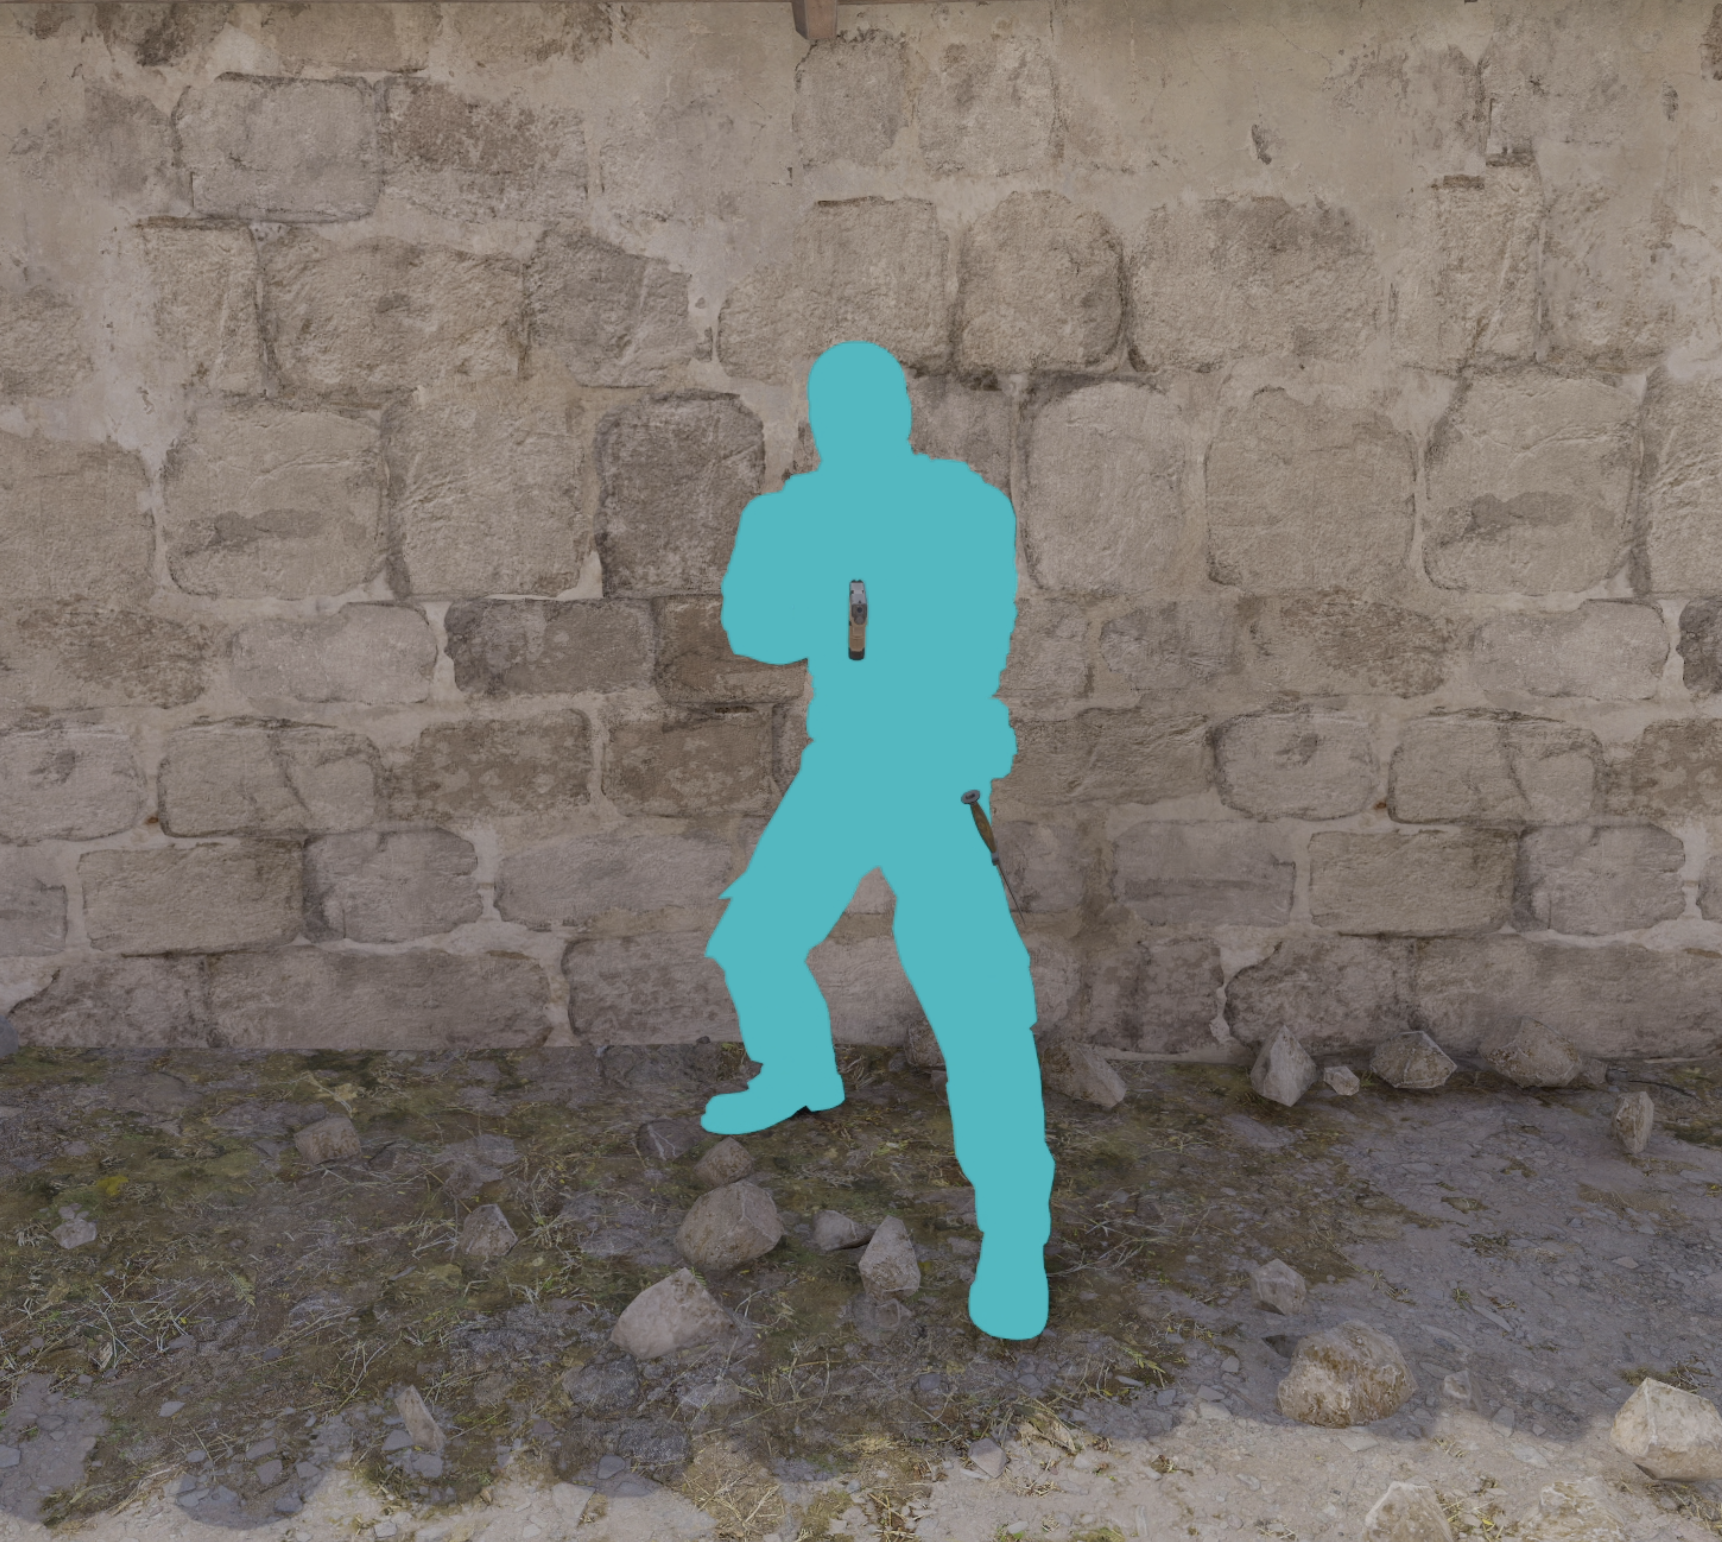
\includegraphics[width=0.3\textwidth,height=0.2\textheight]{images/chams/Screenshot 2025-04-28 at 02.22.38.png}\hspace{1pt}%
    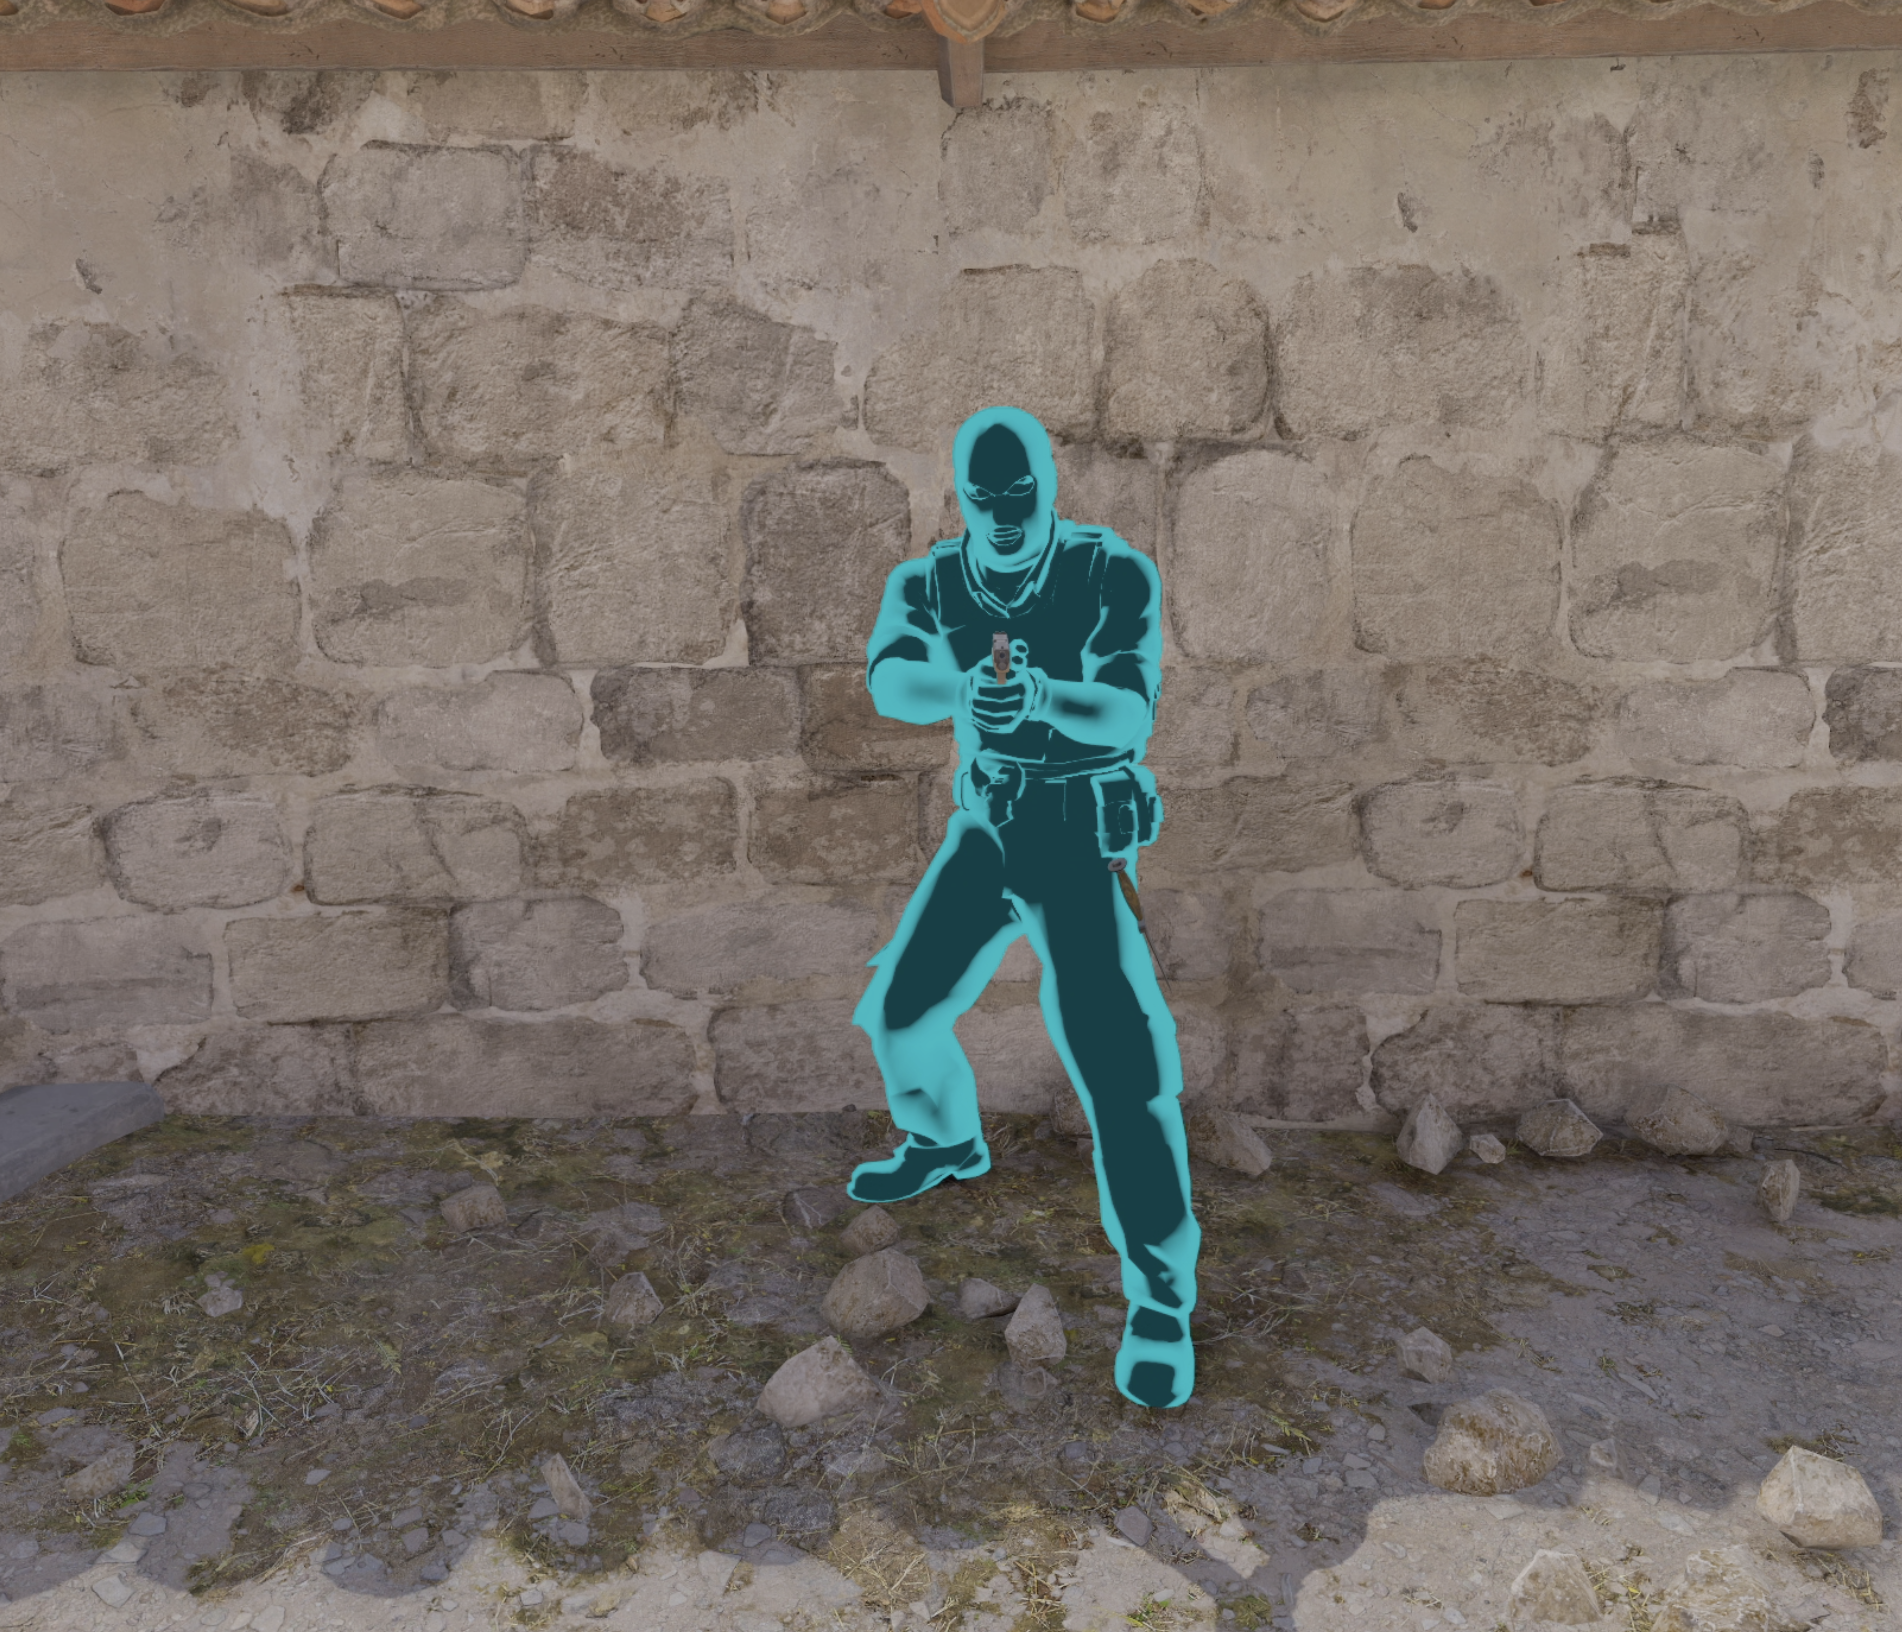
\includegraphics[width=0.3\textwidth,height=0.2\textheight]{images/chams/Screenshot 2025-04-28 at 02.23.03.png}\hspace{1pt}%
    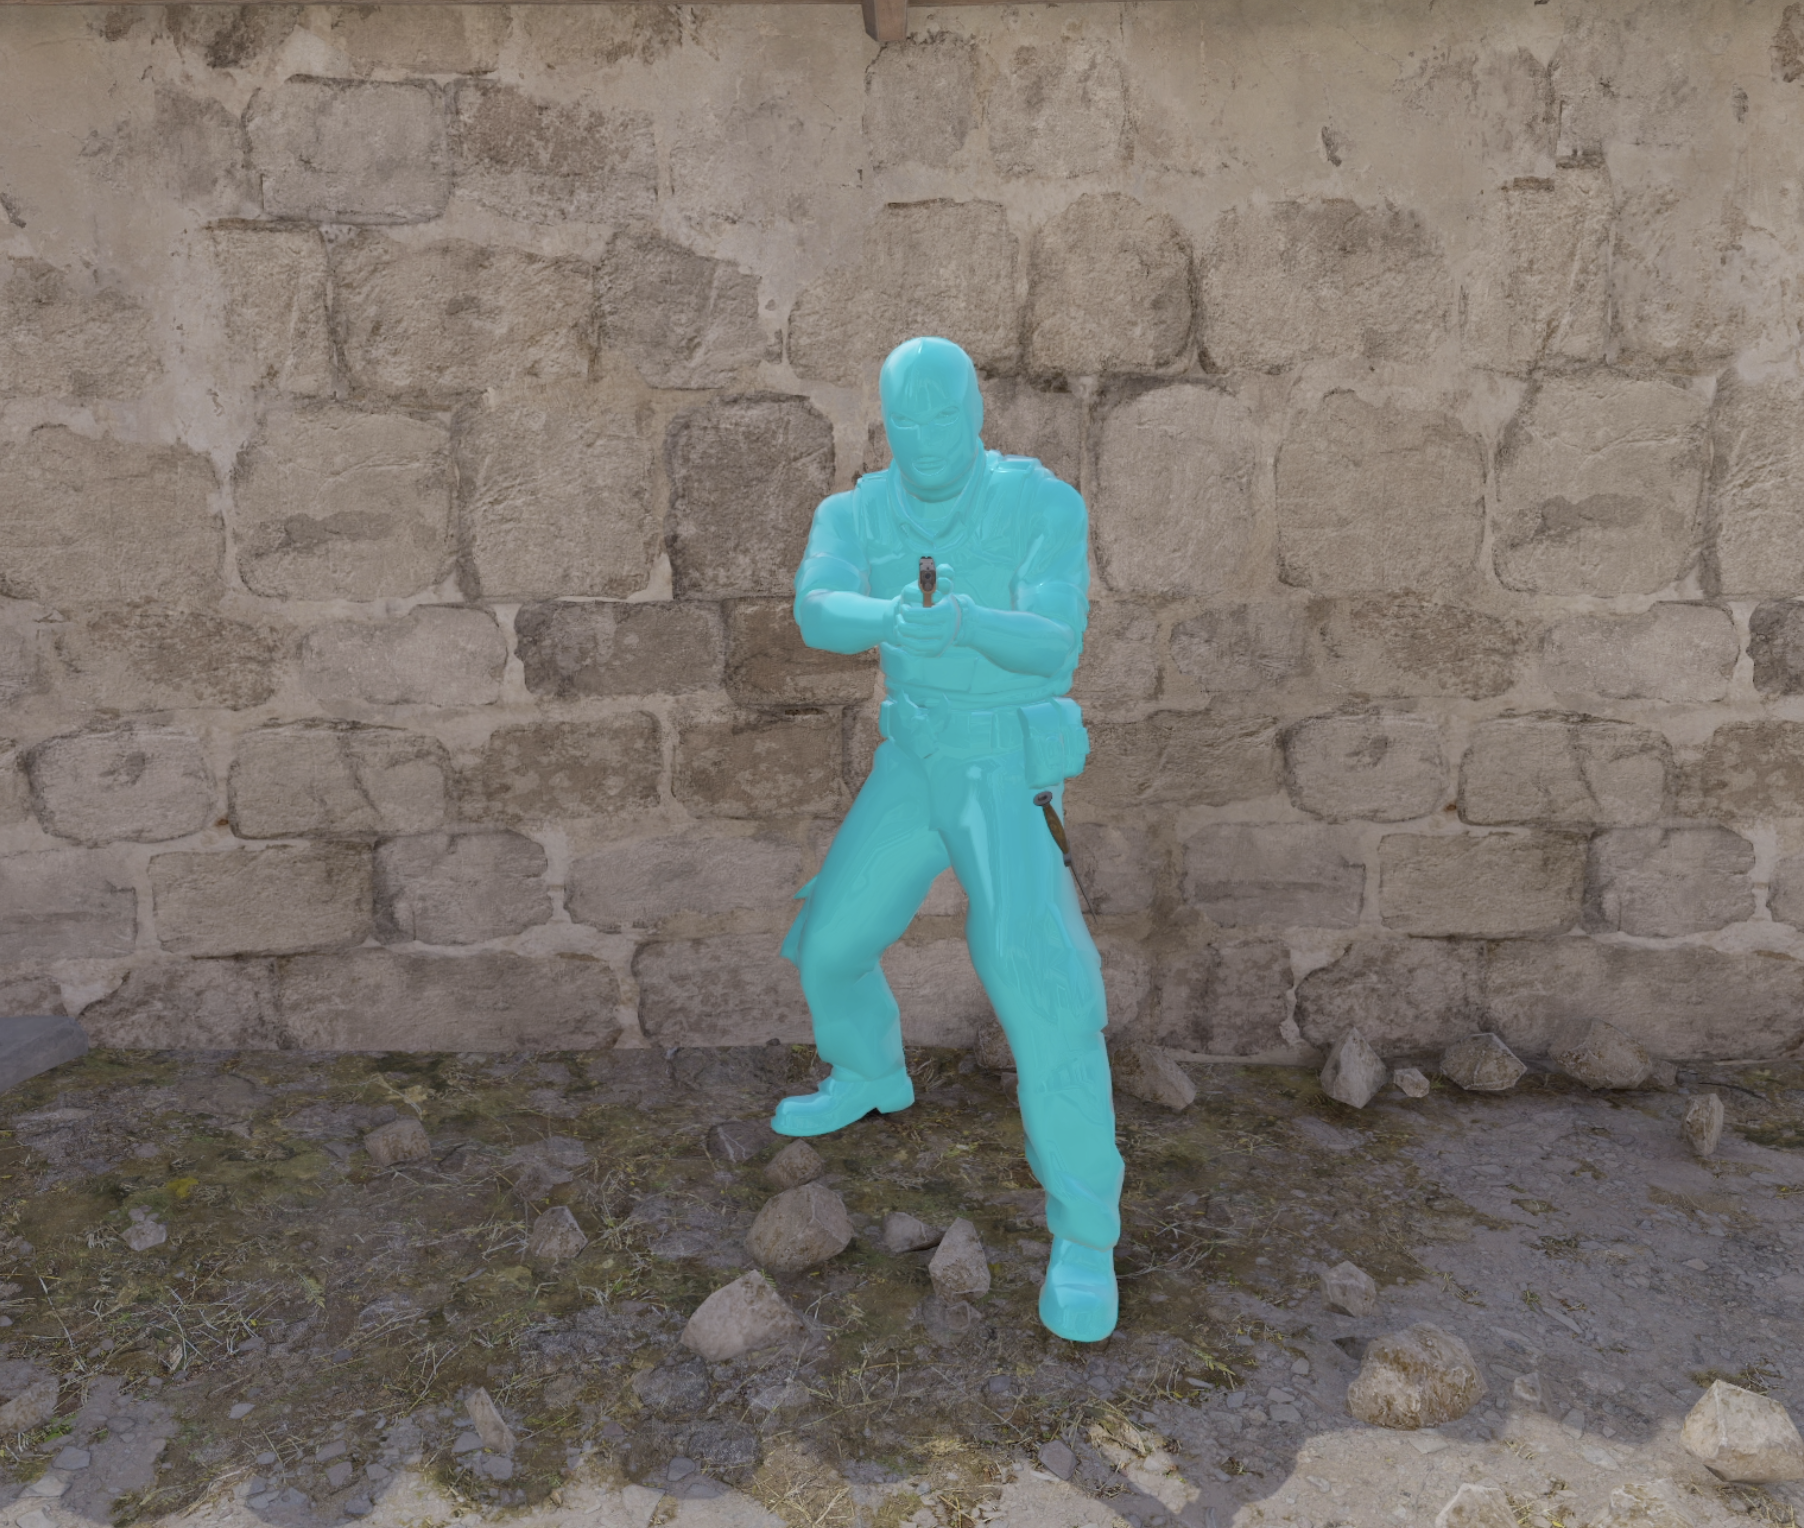
\includegraphics[width=0.3\textwidth,height=0.2\textheight]{images/chams/Screenshot 2025-04-28 at 02.23.29.png}\\[0.2pt]
    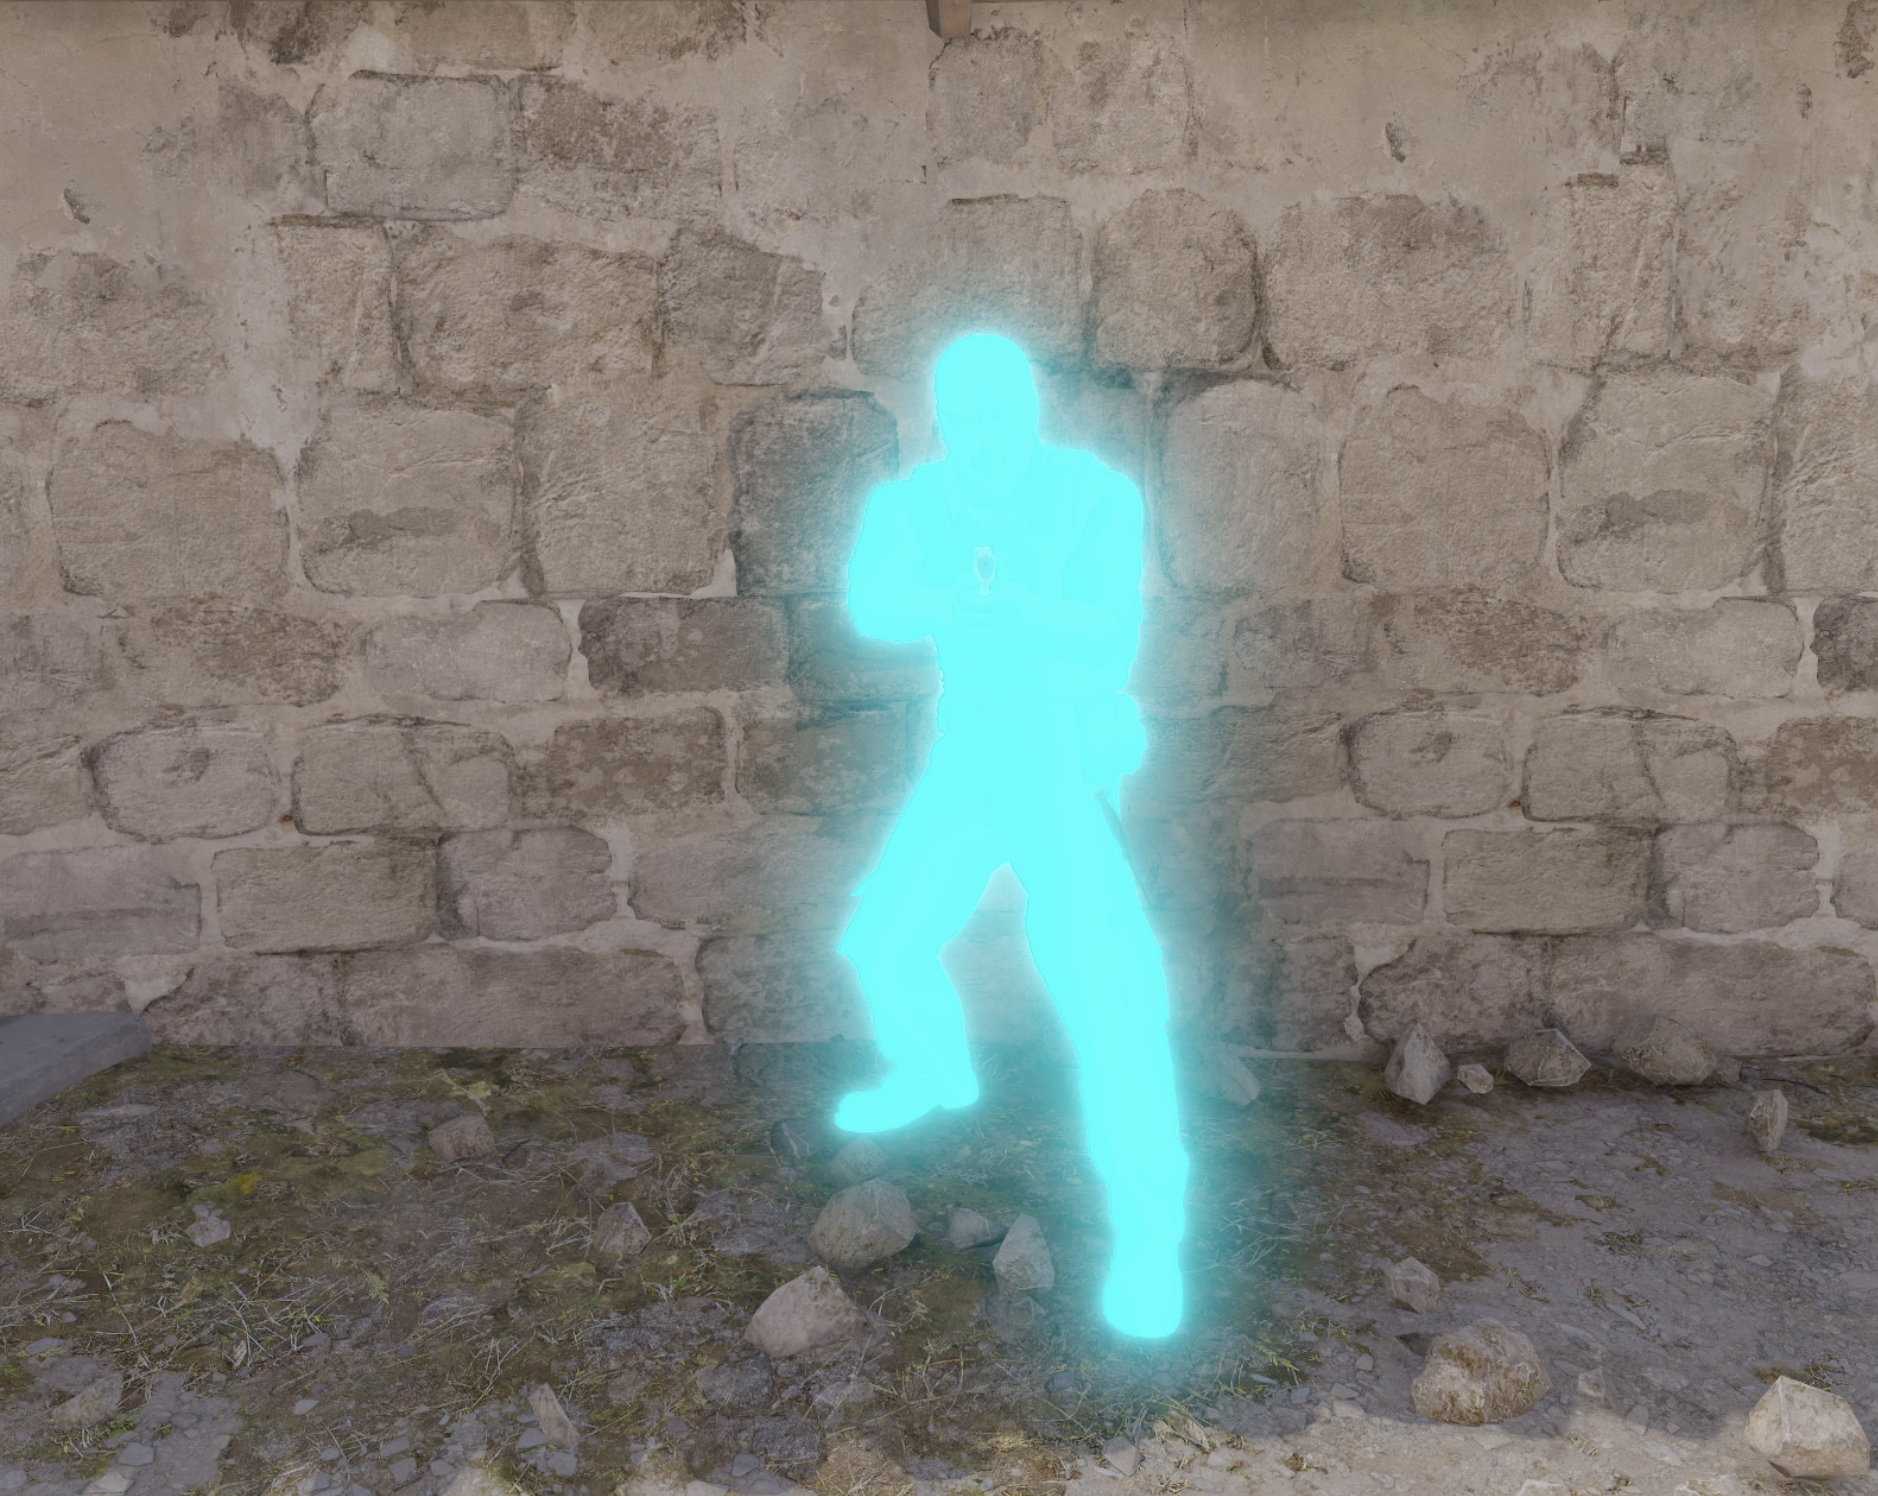
\includegraphics[width=0.3\textwidth,height=0.2\textheight]{images/chams/Screenshot 2025-04-28 at 02.24.15.png}\hspace{1pt}%
    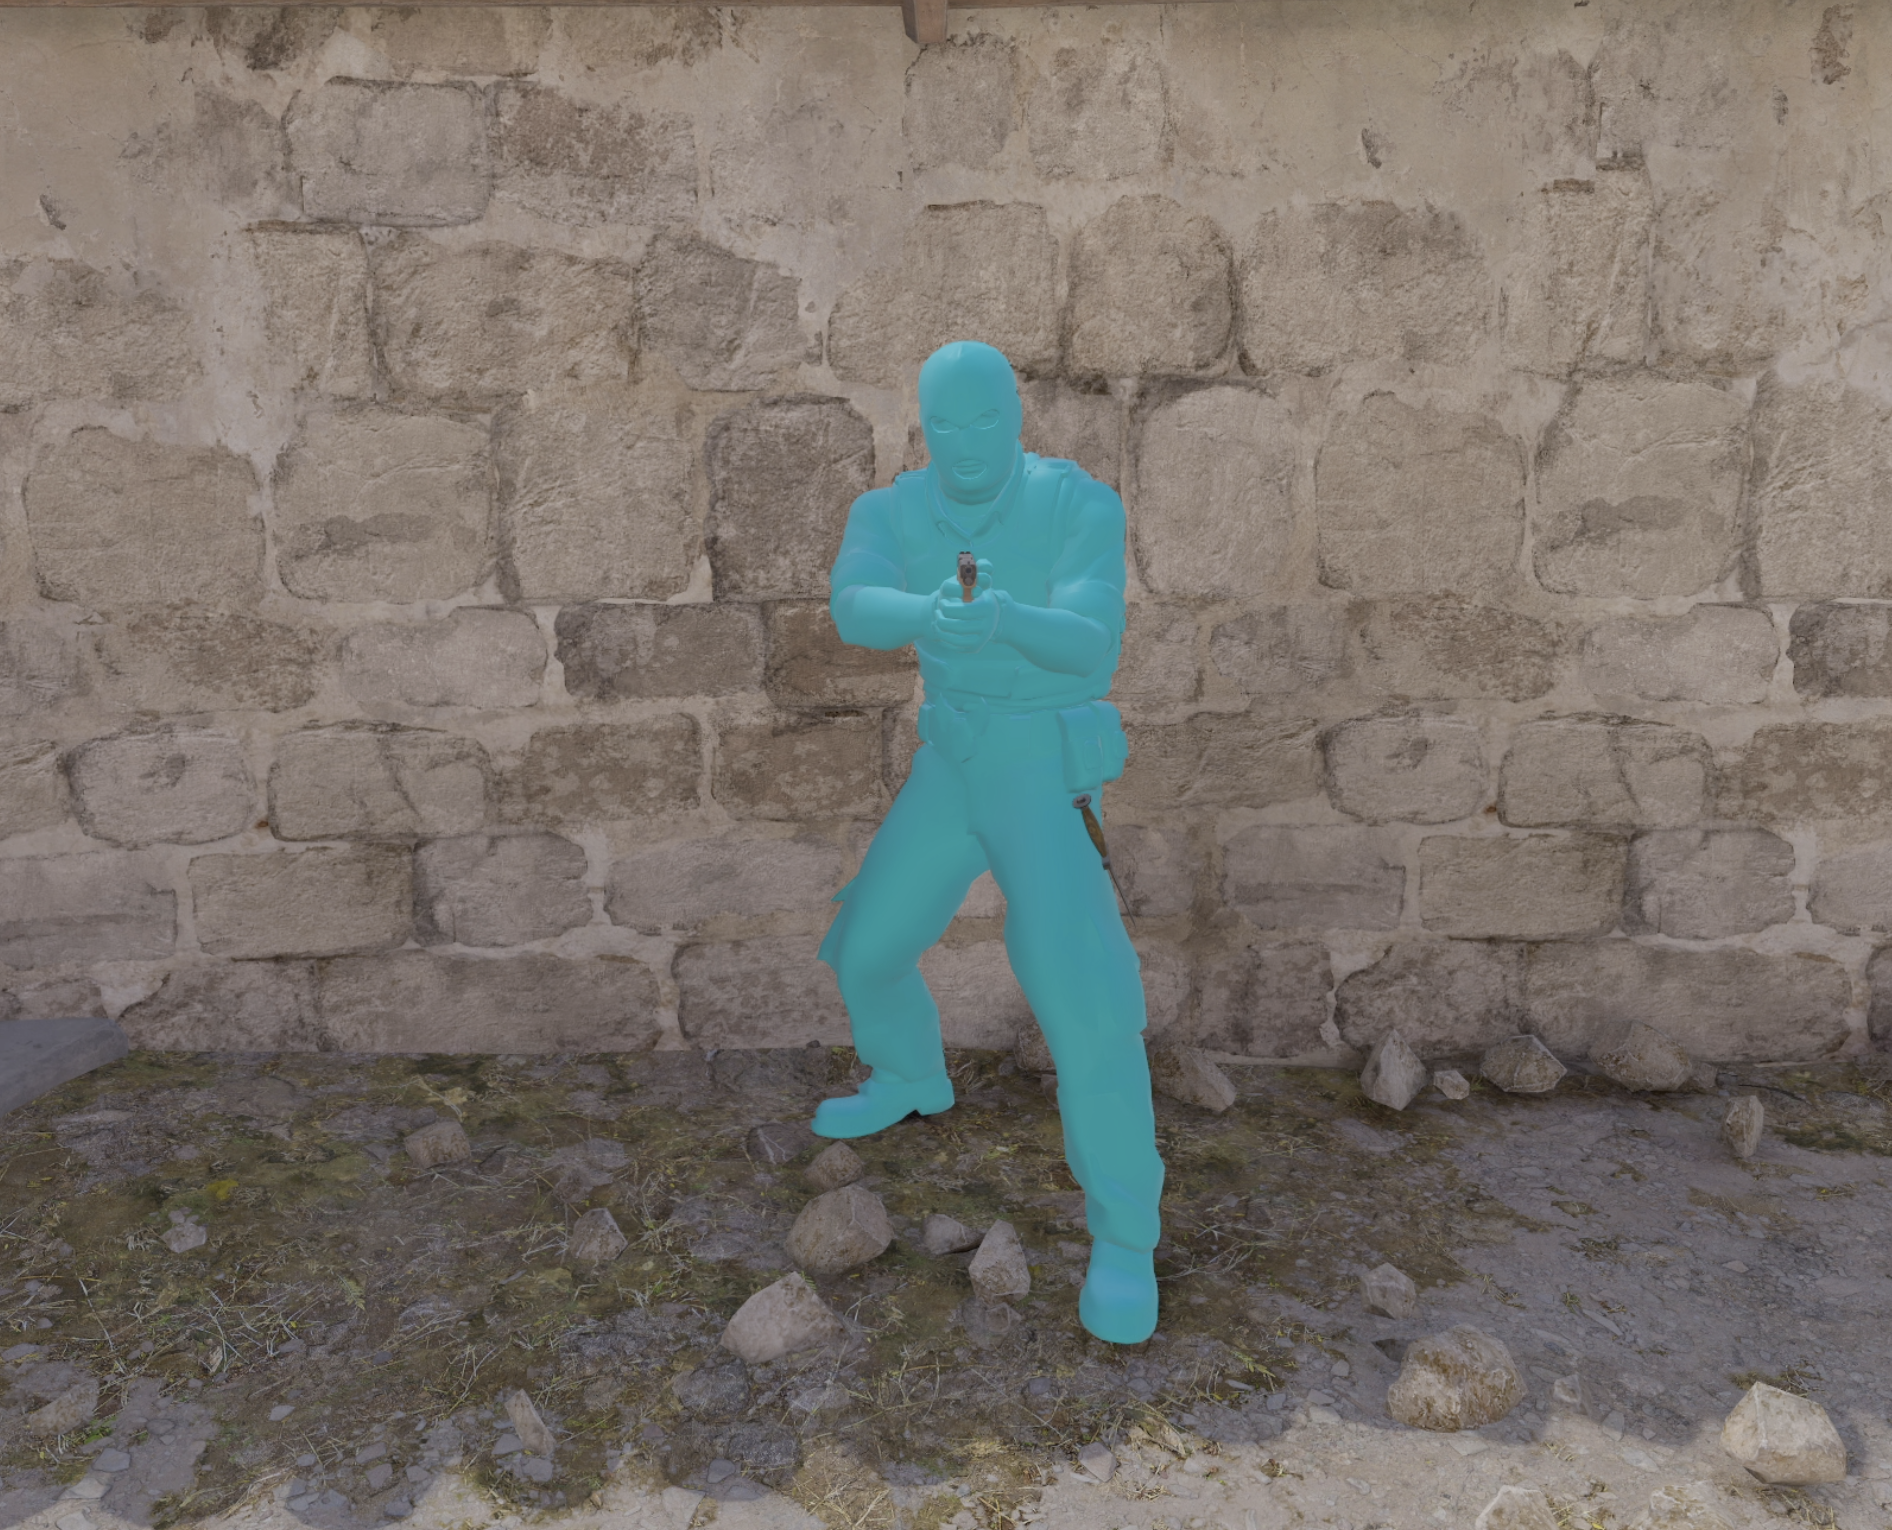
\includegraphics[width=0.3\textwidth,height=0.2\textheight]{images/chams/Screenshot 2025-04-28 at 02.23.53.png}\hspace{1pt}%
    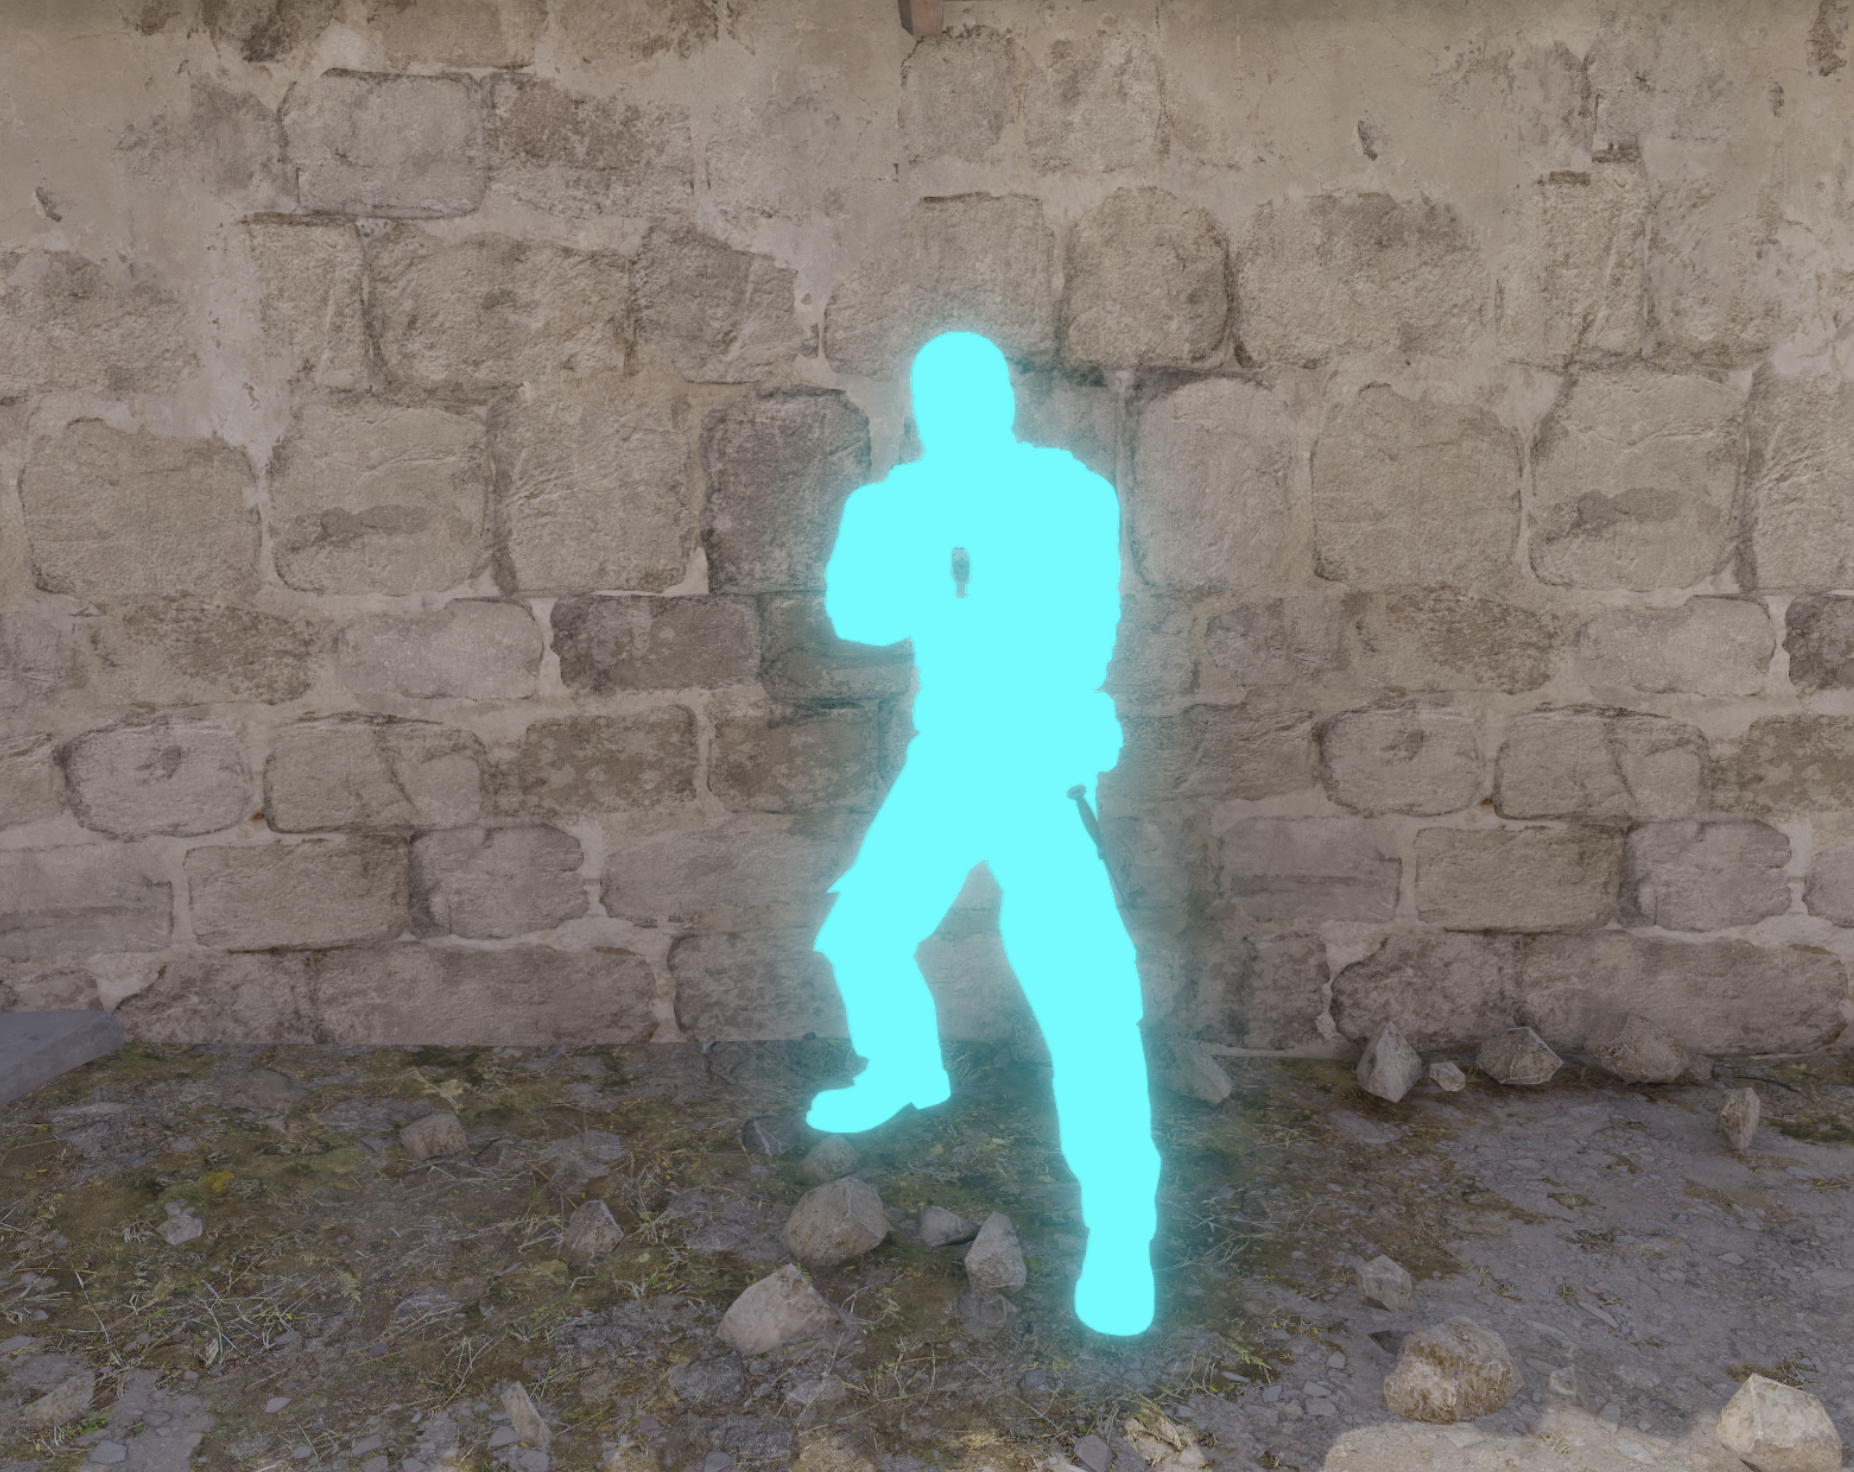
\includegraphics[width=0.3\textwidth,height=0.2\textheight]{images/chams/Screenshot 2025-04-28 at 02.24.33.png}        
    \caption{Different Chams materials rendered with blue tones.}
\end{figure}

\begin{figure}[H]
    \centering
    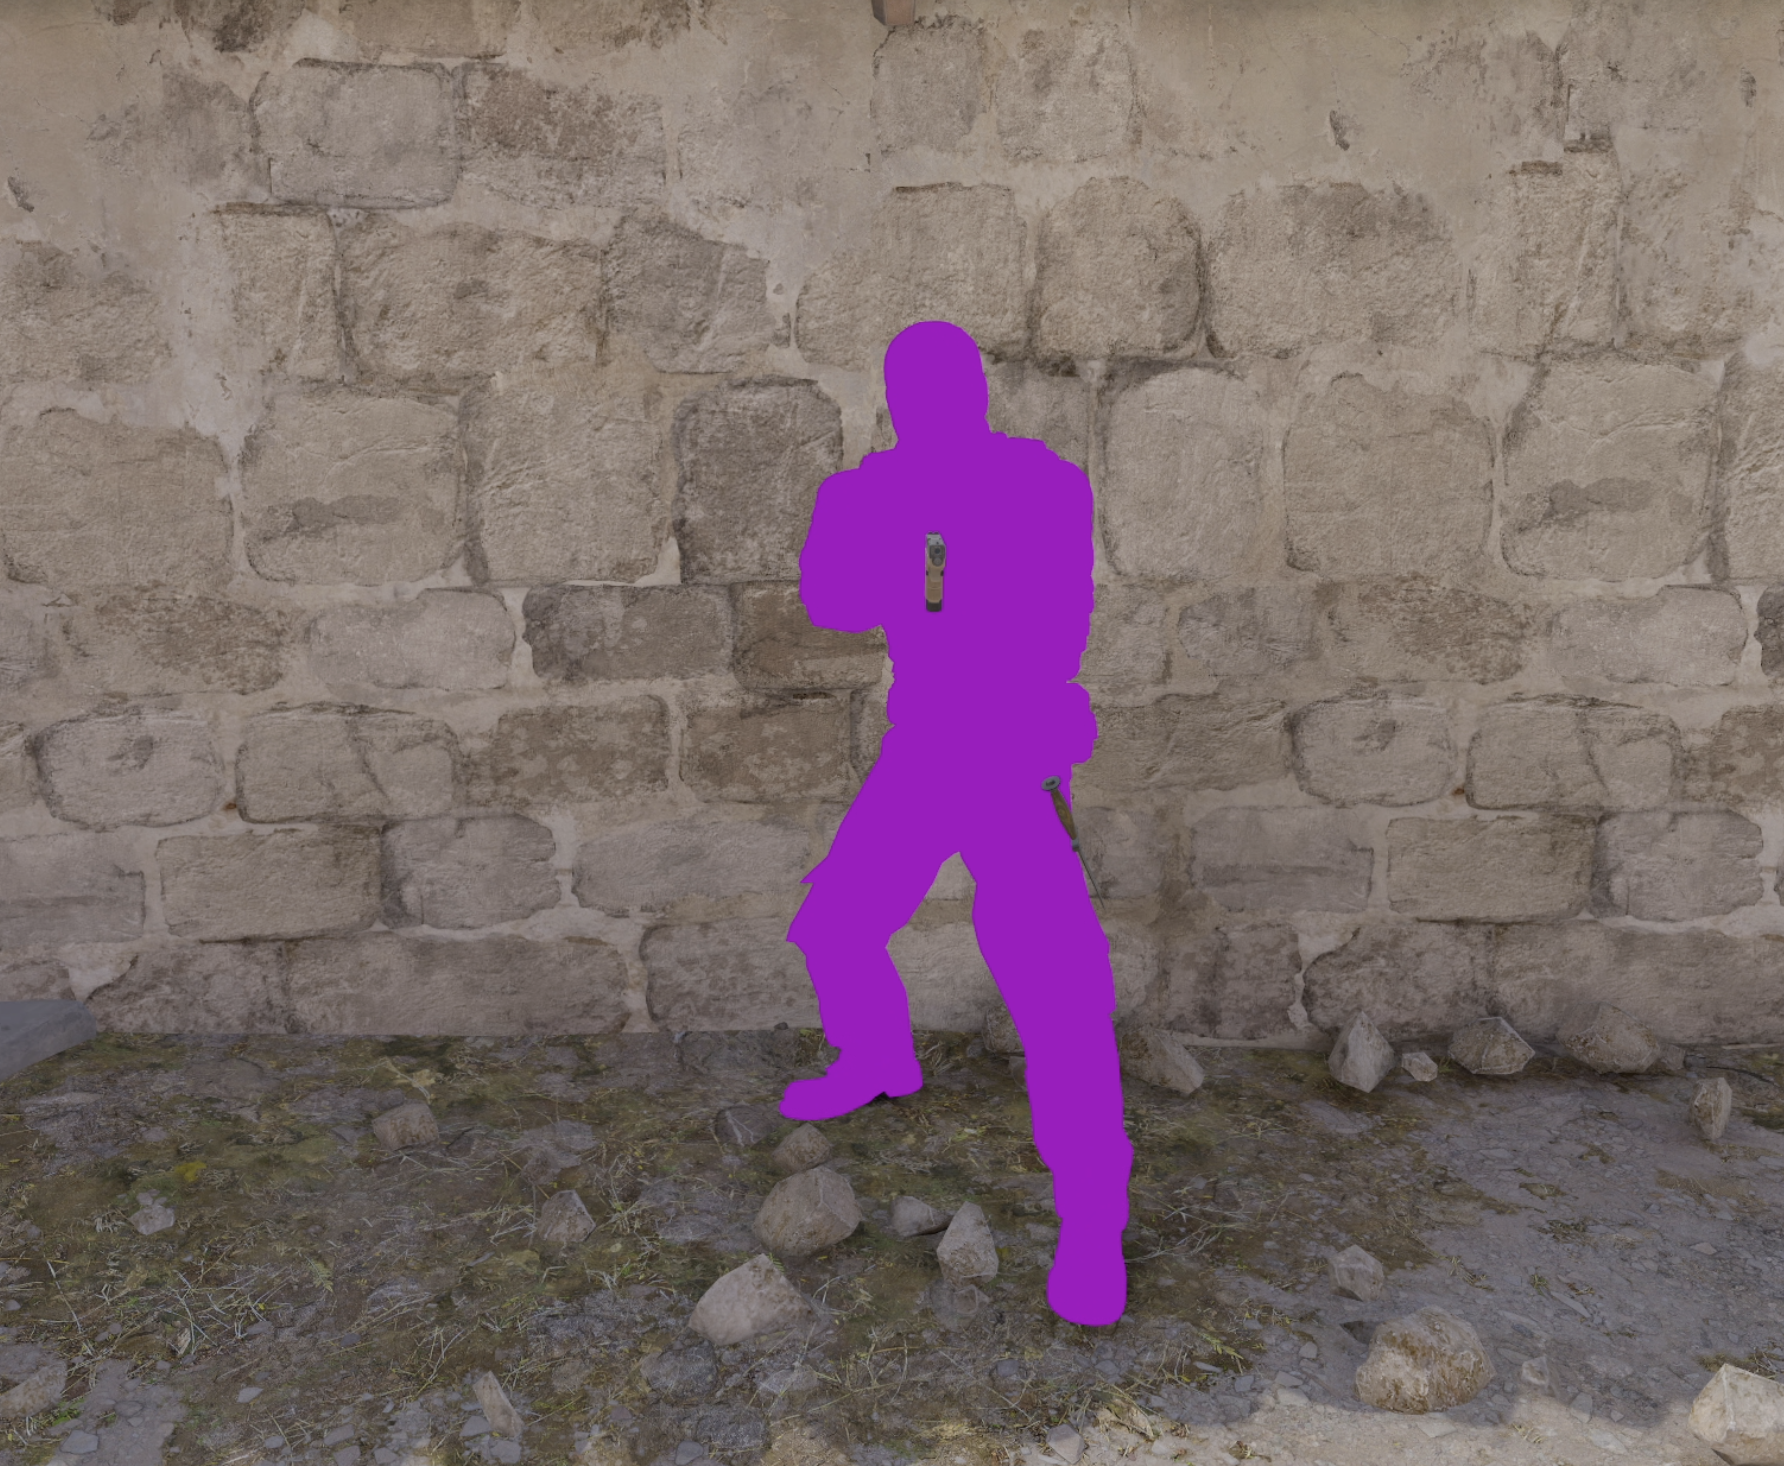
\includegraphics[width=0.3\textwidth,height=0.20\textheight]{images/chams/Screenshot 2025-04-28 at 02.25.09.png}\hspace{1pt}%
    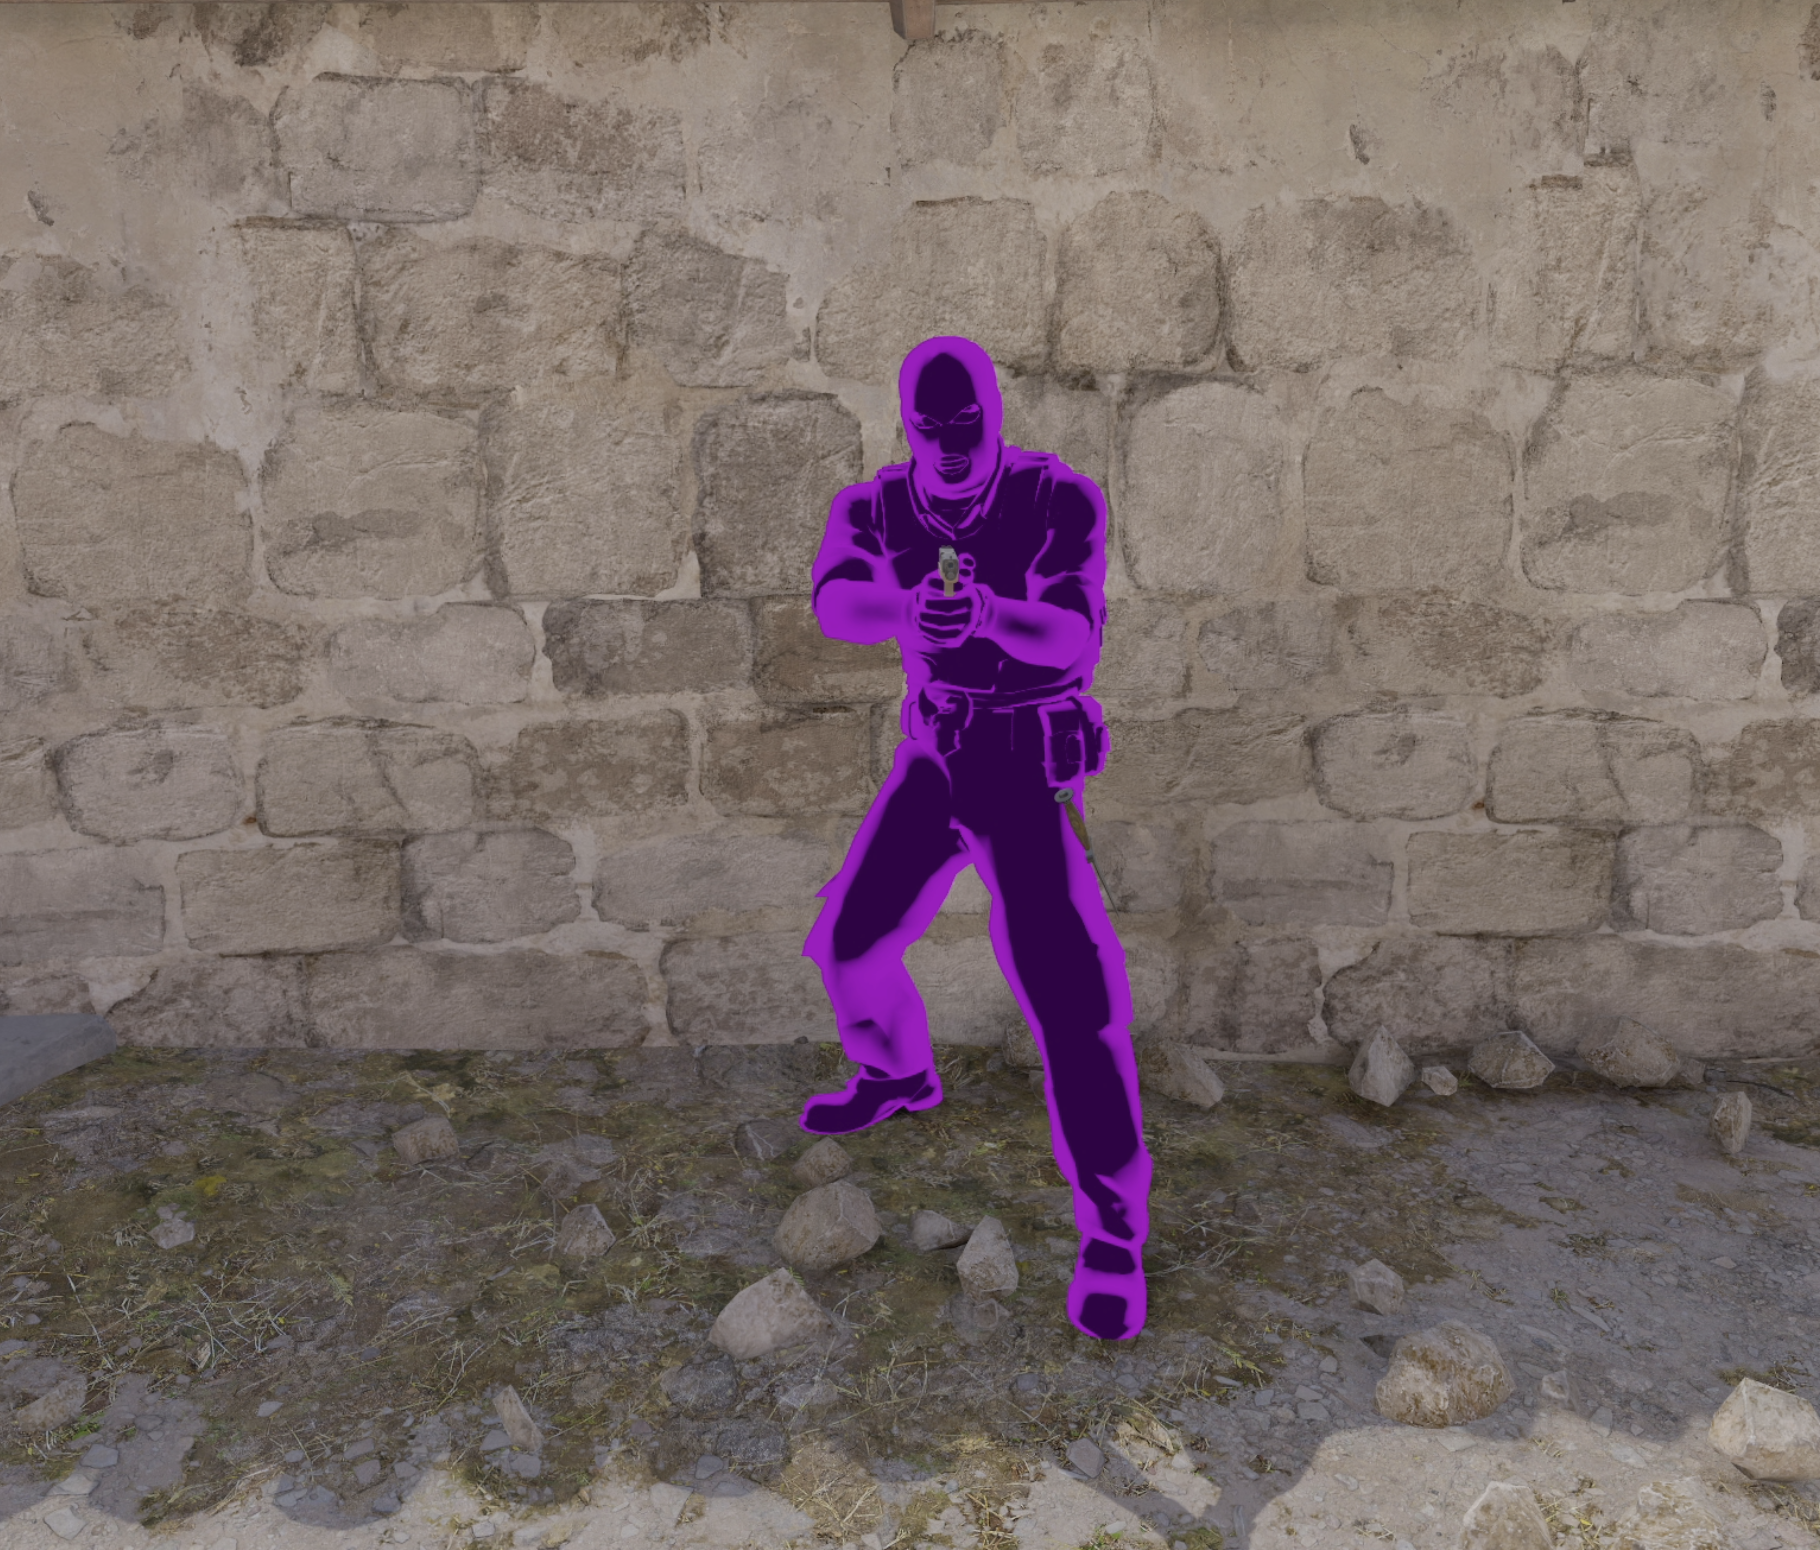
\includegraphics[width=0.3\textwidth,height=0.20\textheight]{images/chams/Screenshot 2025-04-28 at 02.25.31.png}\hspace{1pt}%
    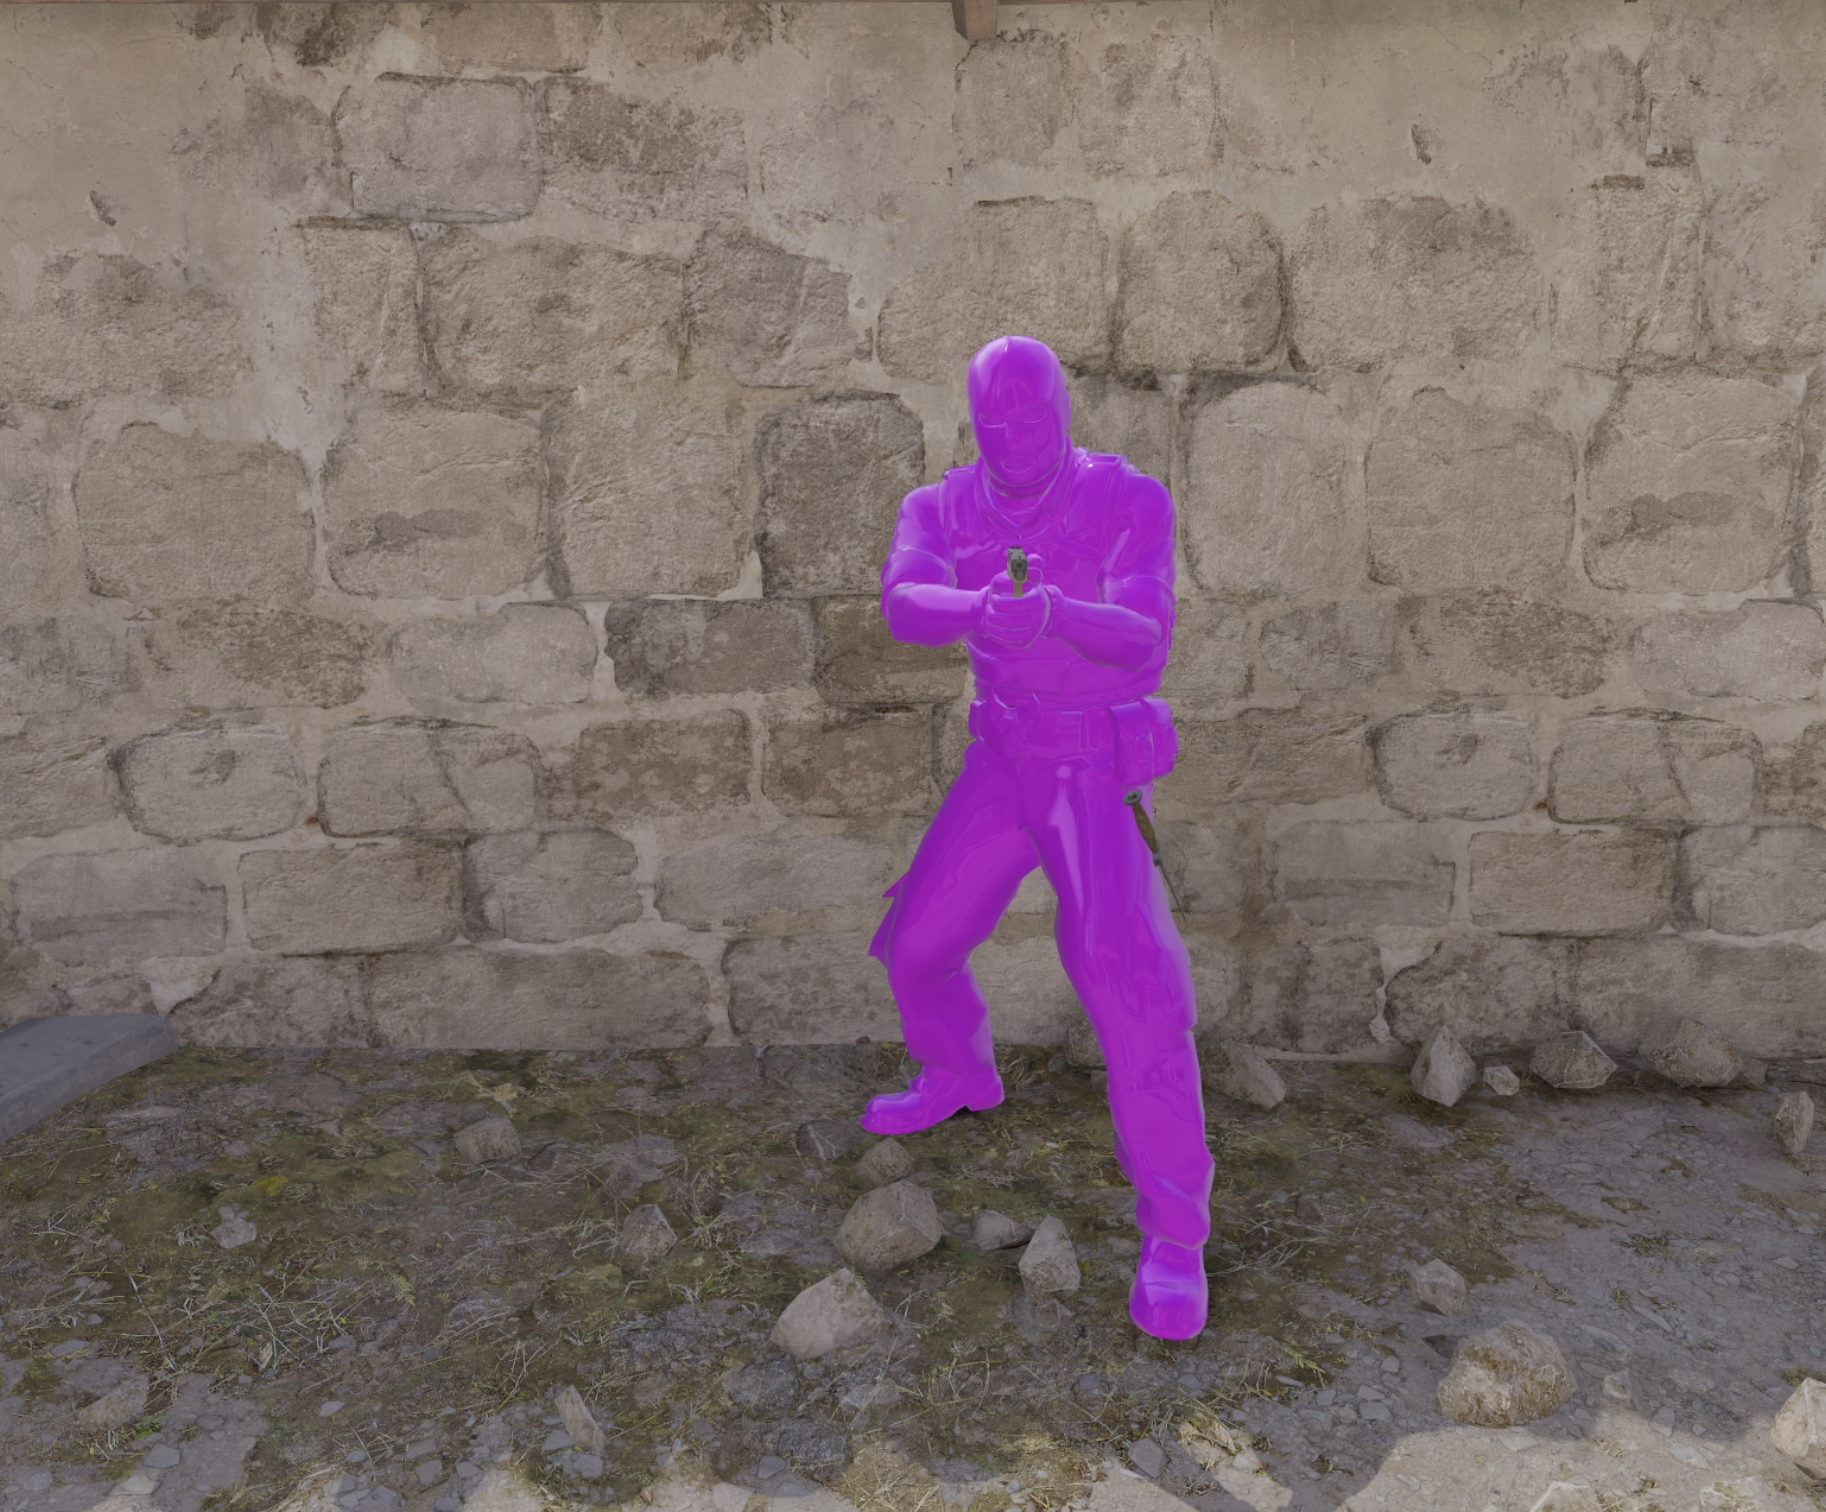
\includegraphics[width=0.3\textwidth,height=0.20\textheight]{images/chams/Screenshot 2025-04-28 at 02.25.47.png}\\[0.2pt]
    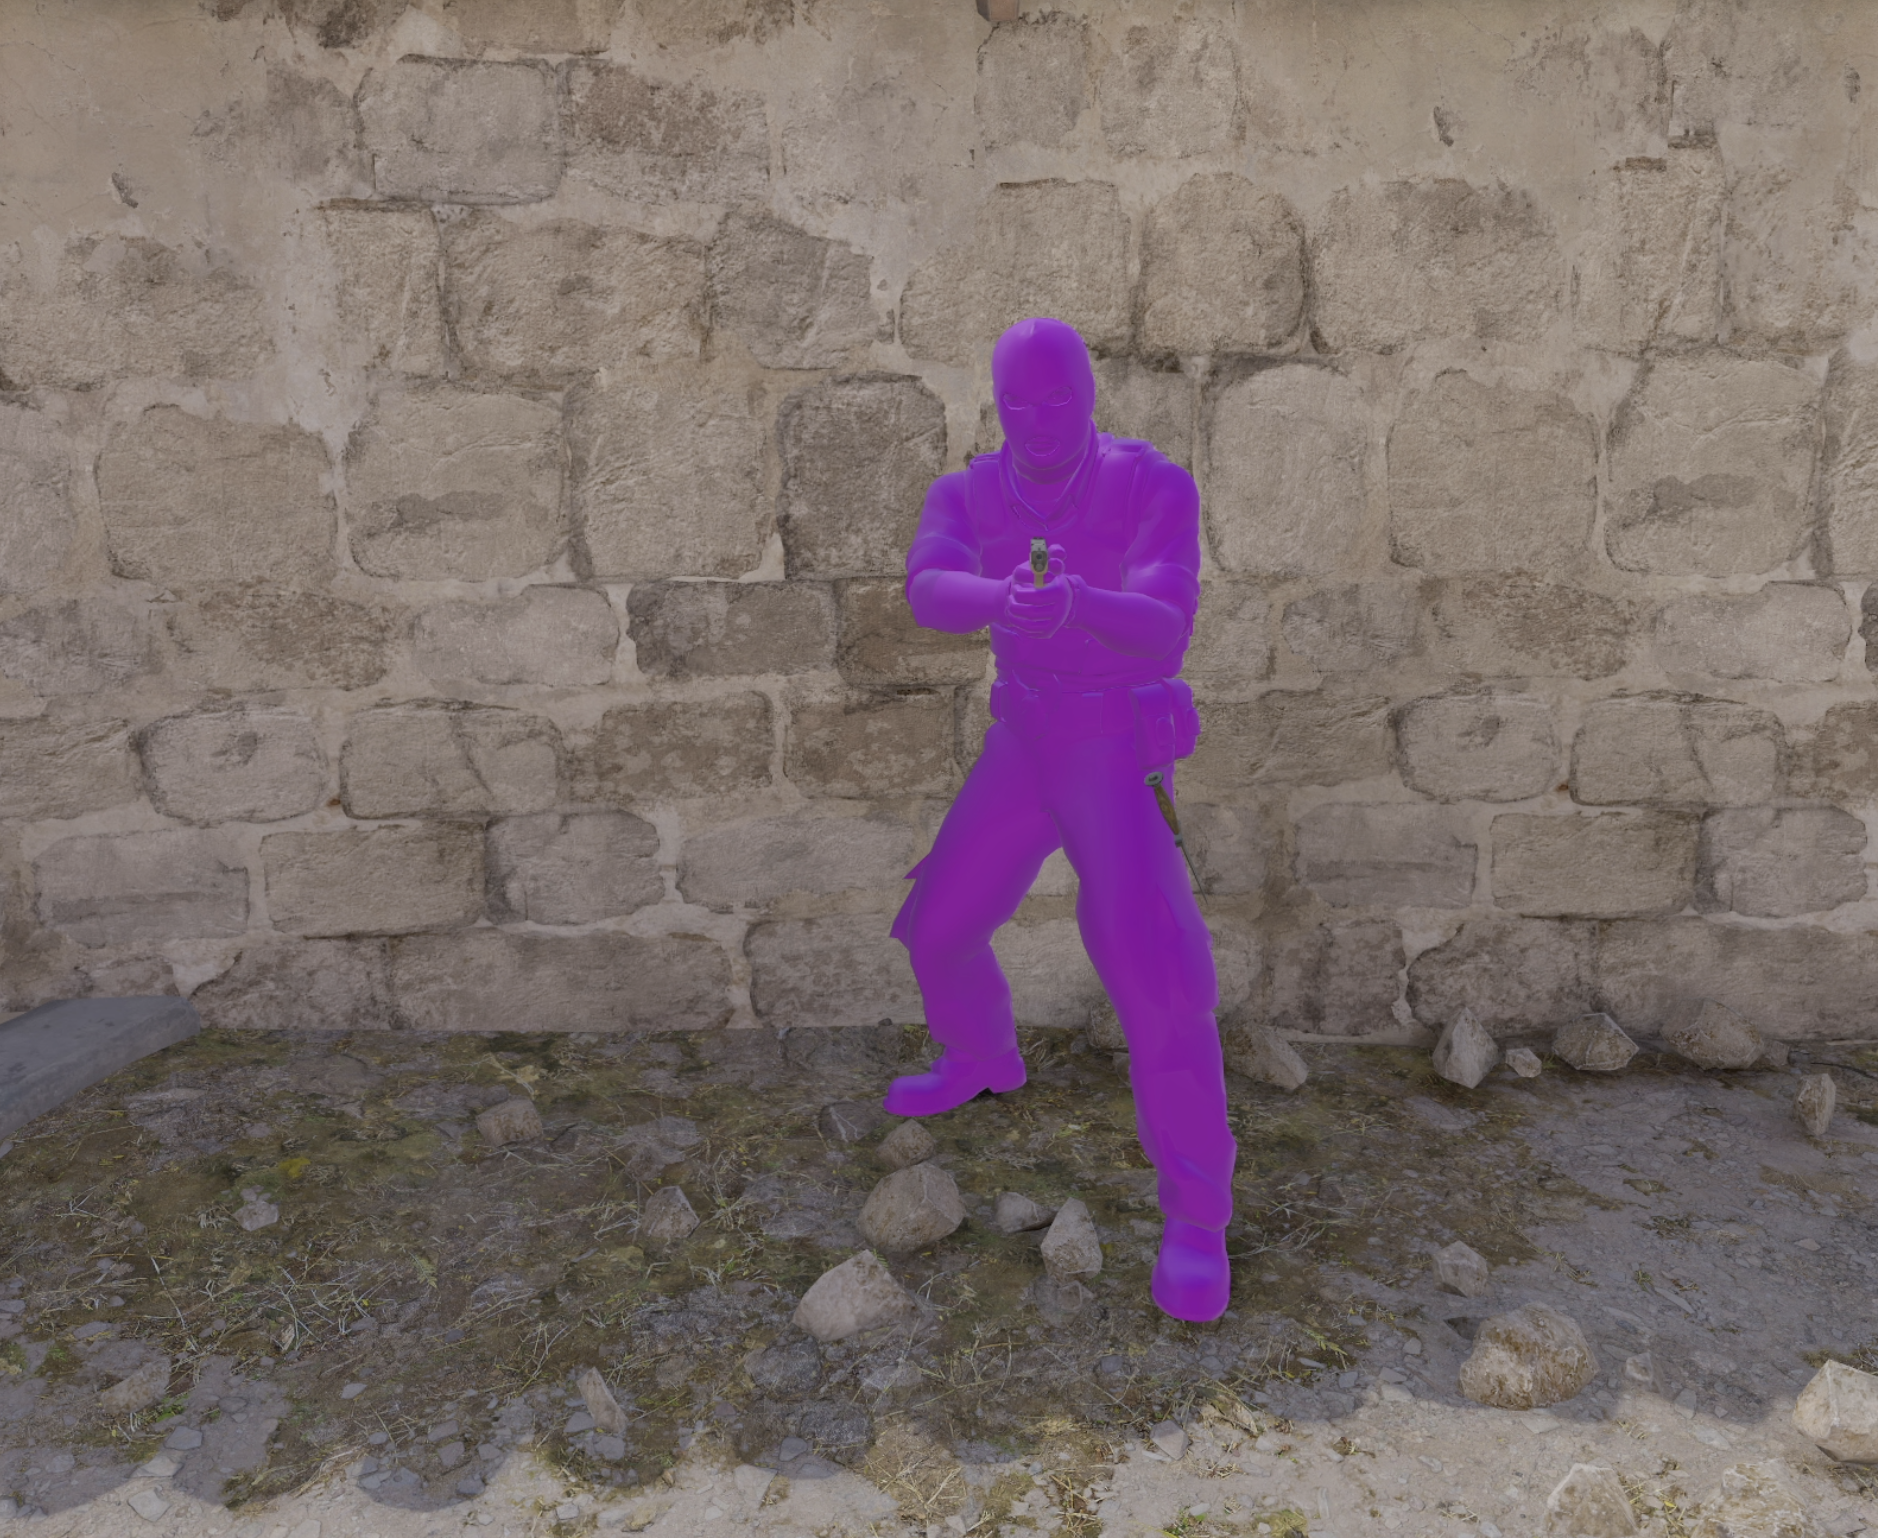
\includegraphics[width=0.3\textwidth,height=0.20\textheight]{images/chams/Screenshot 2025-04-28 at 02.26.01.png}\hspace{1pt}%
    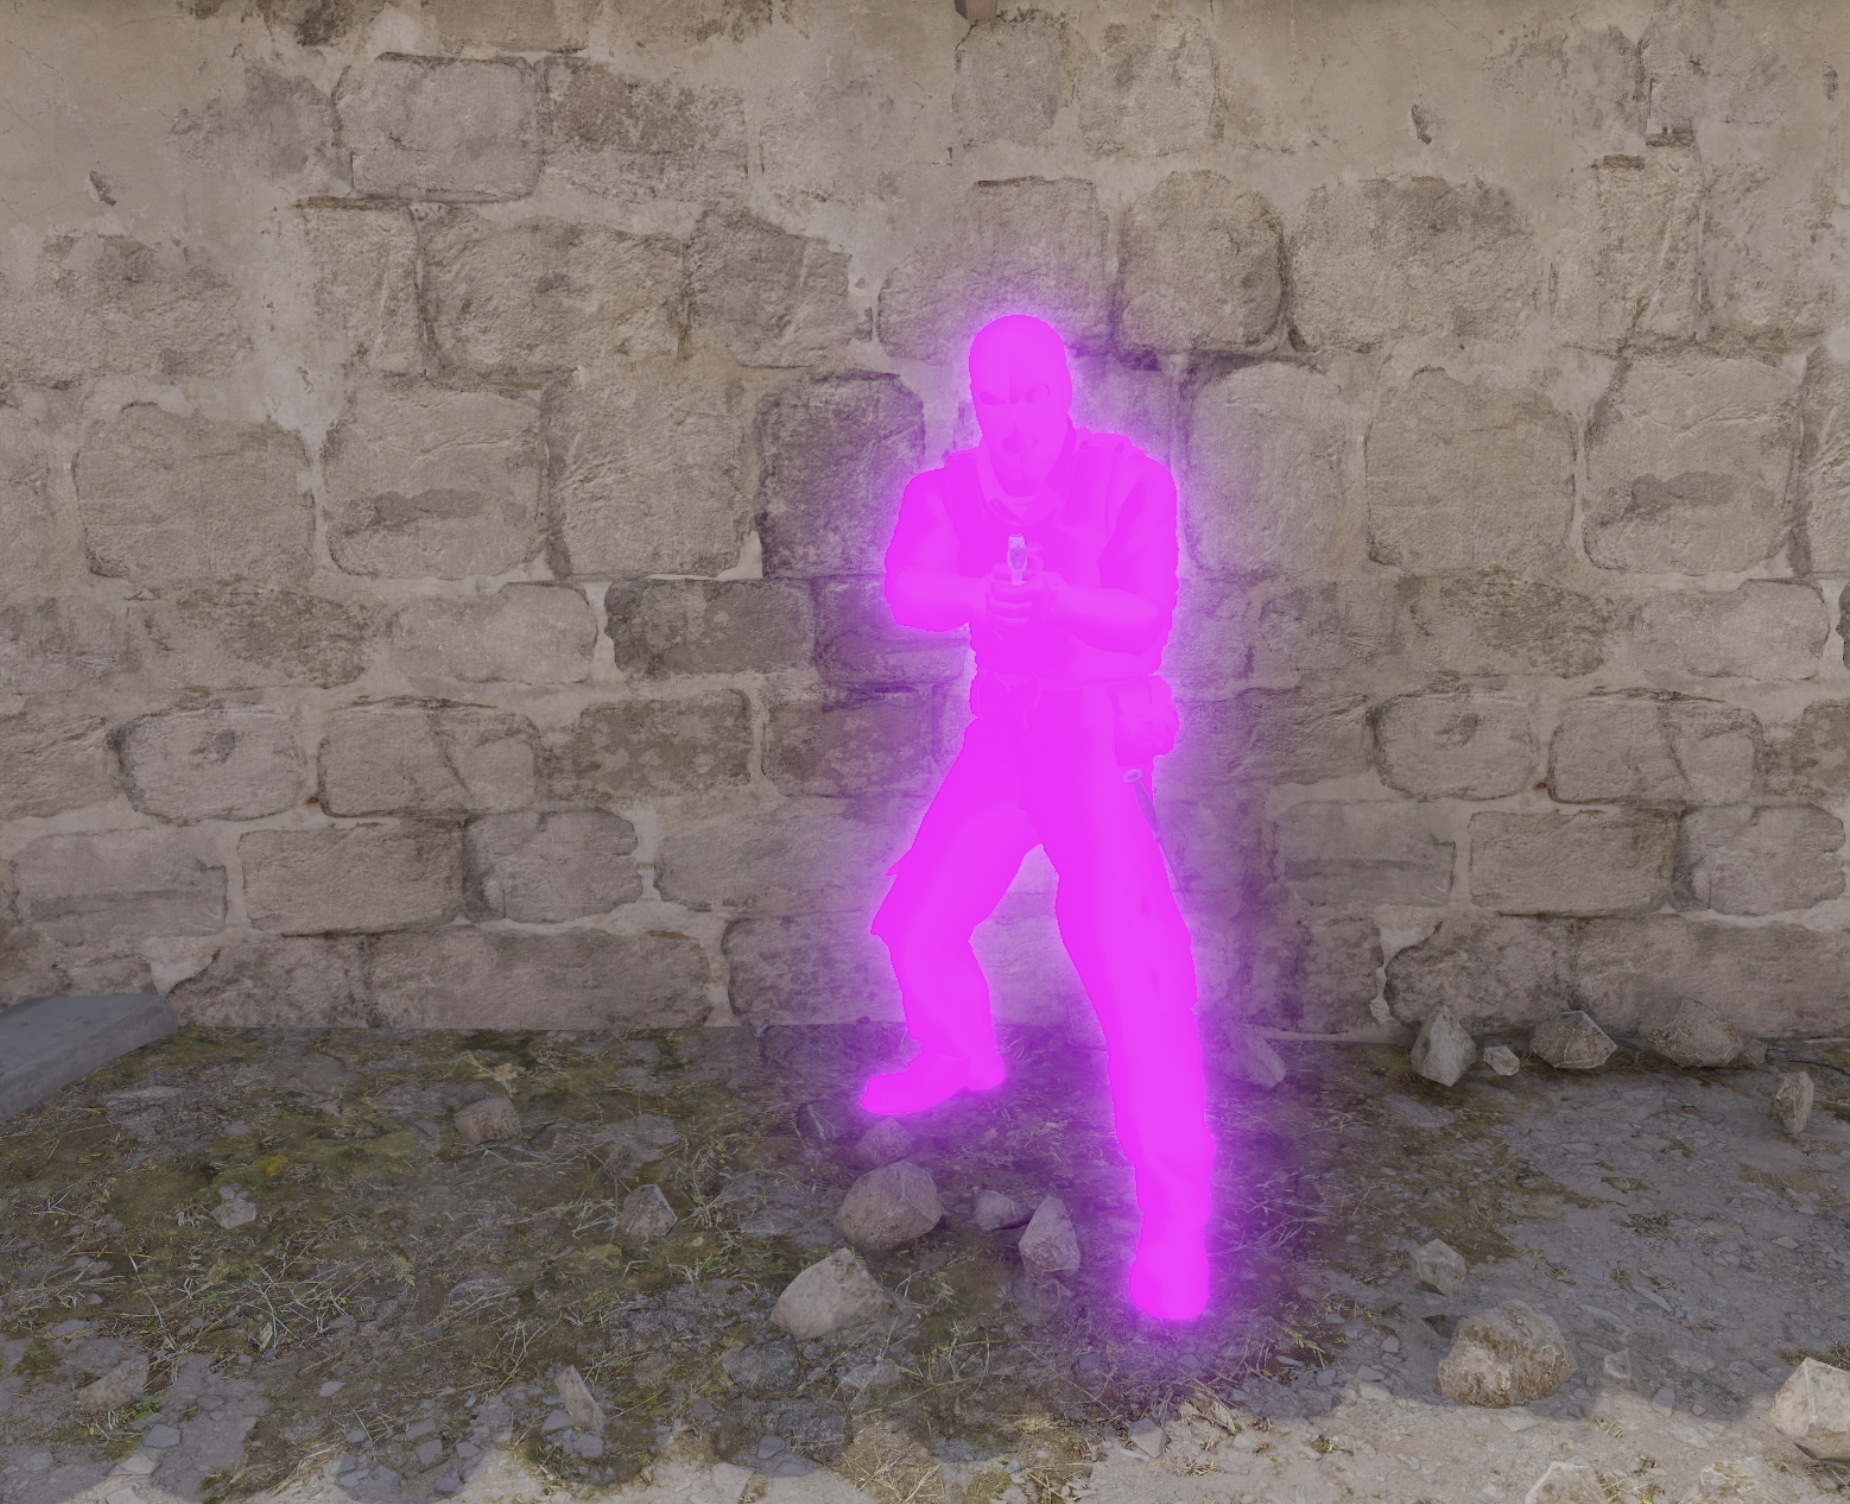
\includegraphics[width=0.3\textwidth,height=0.20\textheight]{images/chams/Screenshot 2025-04-28 at 02.26.14.png}\hspace{1pt}%
    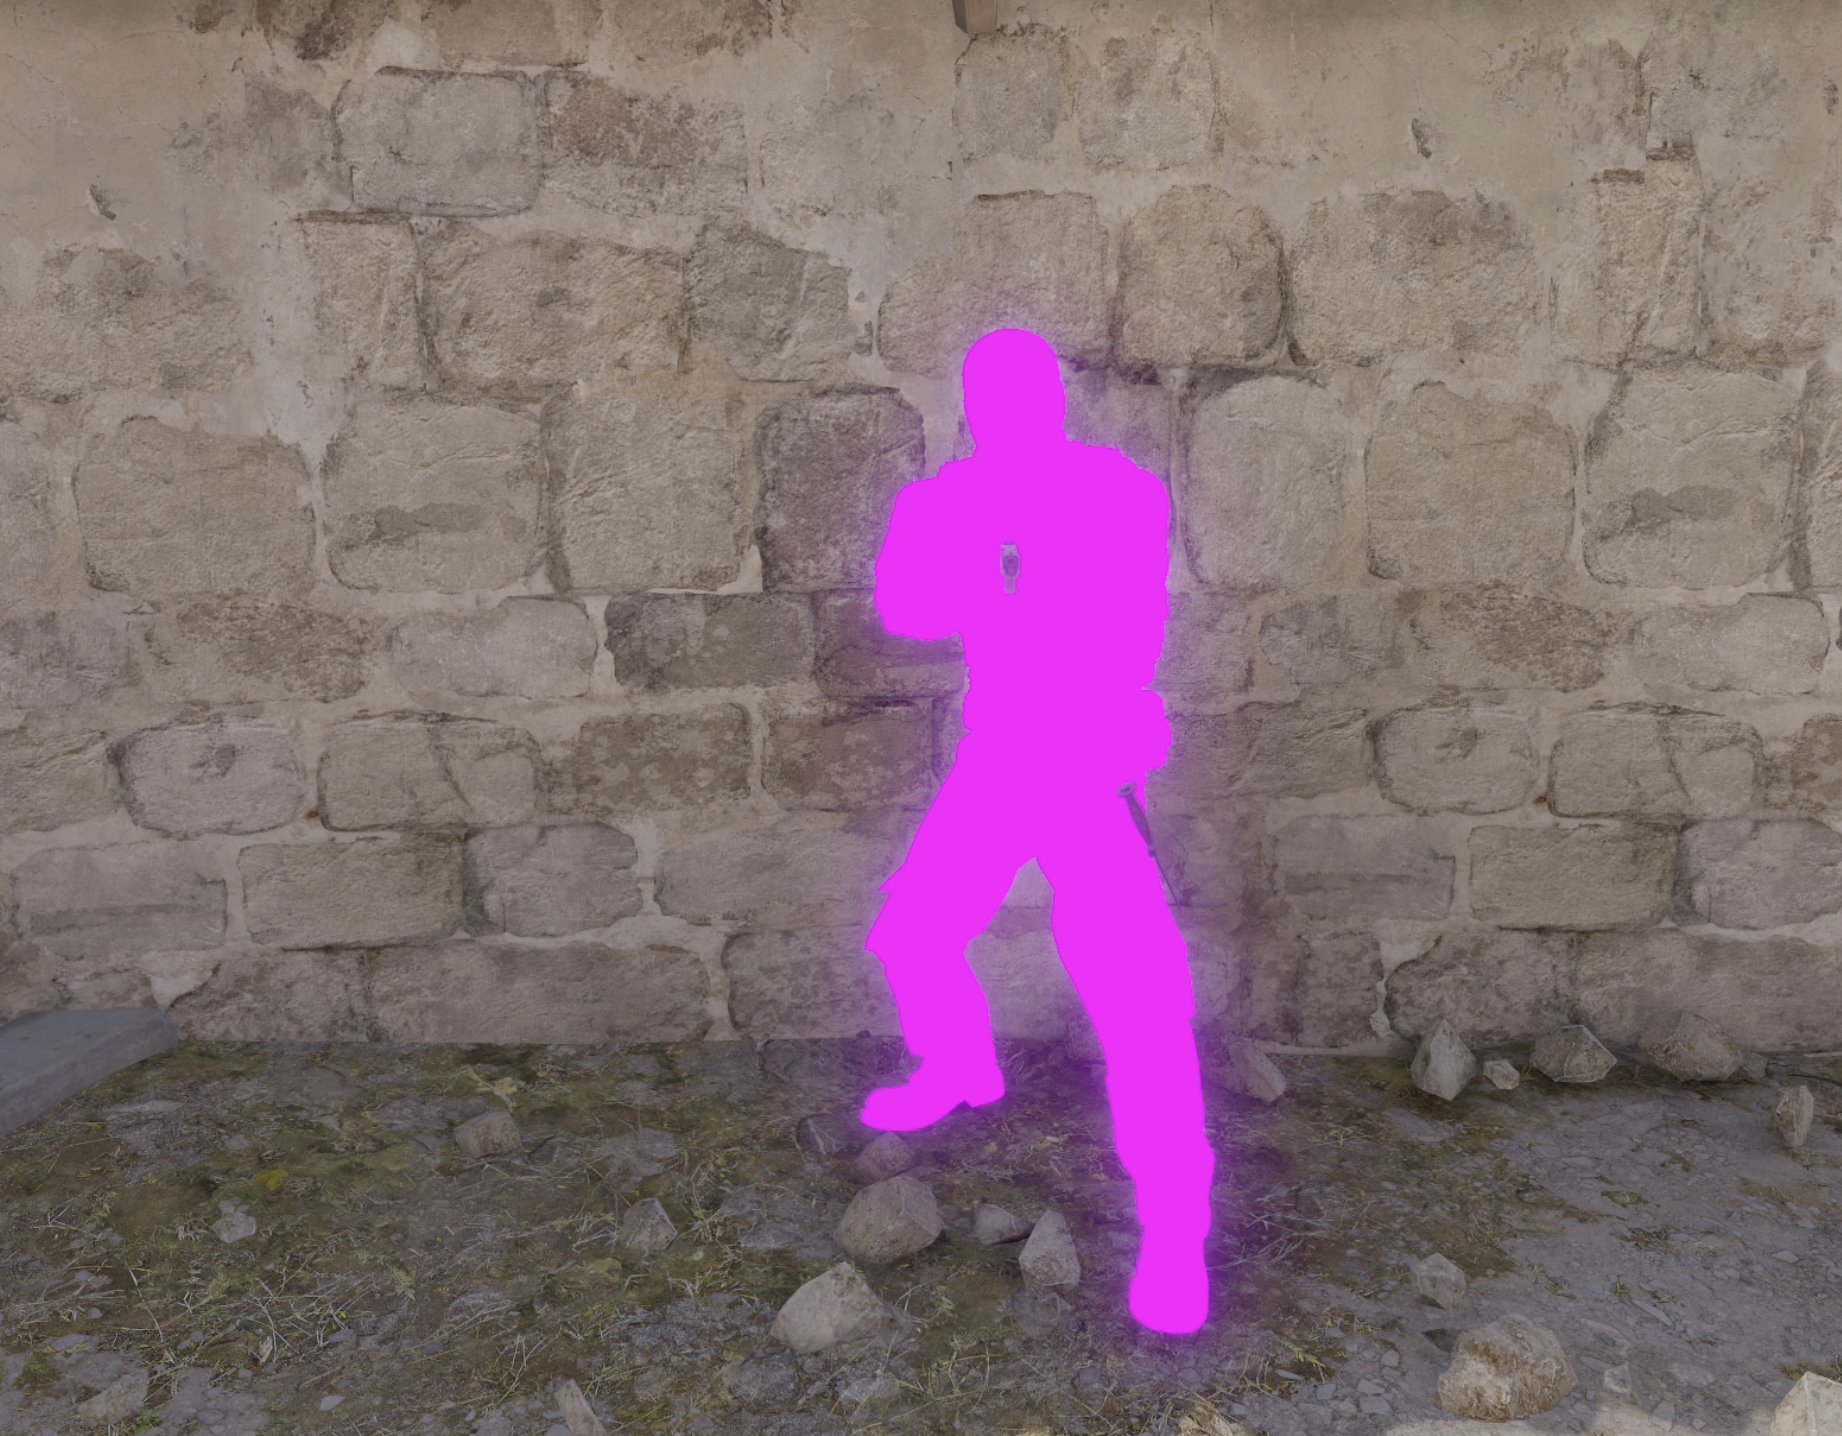
\includegraphics[width=0.3\textwidth,height=0.20\textheight]{images/chams/Screenshot 2025-04-28 at 02.26.29.png}
    \caption{Different Chams materials rendered with purple tones.}
\end{figure}



\subsubsection{Visible vs Non-Visible Chams Logic}

Once this logic is in place, we can take it a step further and assign different materials to the visible and non-visible parts of the enemy player model. This allows us to render, for example, the visible part of the player in one color (e.g., purple) and the non-visible part (e.g., behind walls) in another (e.g., yellow). 

Since this rendering is only visible locally to the cheat user and not to other players in the match, it enables us to appear as a legitimate player with significantly better awareness and reflexes. By clearly seeing which parts of an enemy are exposed and which are not, we can ensure to only target the visible areas.

This reduces the risk of suspicious-looking shots (such as pre-firing through walls or headshots through solid cover) and helps us maintain a "legit" playstyle that blends in with skilled human behavior. In turn, this greatly decreases the chances of triggering manual bans during demo reviews or overwatch-like systems, where human moderators could flag unnatural behavior.

\begin{figure}[H]
    \centering

    \makebox[\textwidth][c]{%
        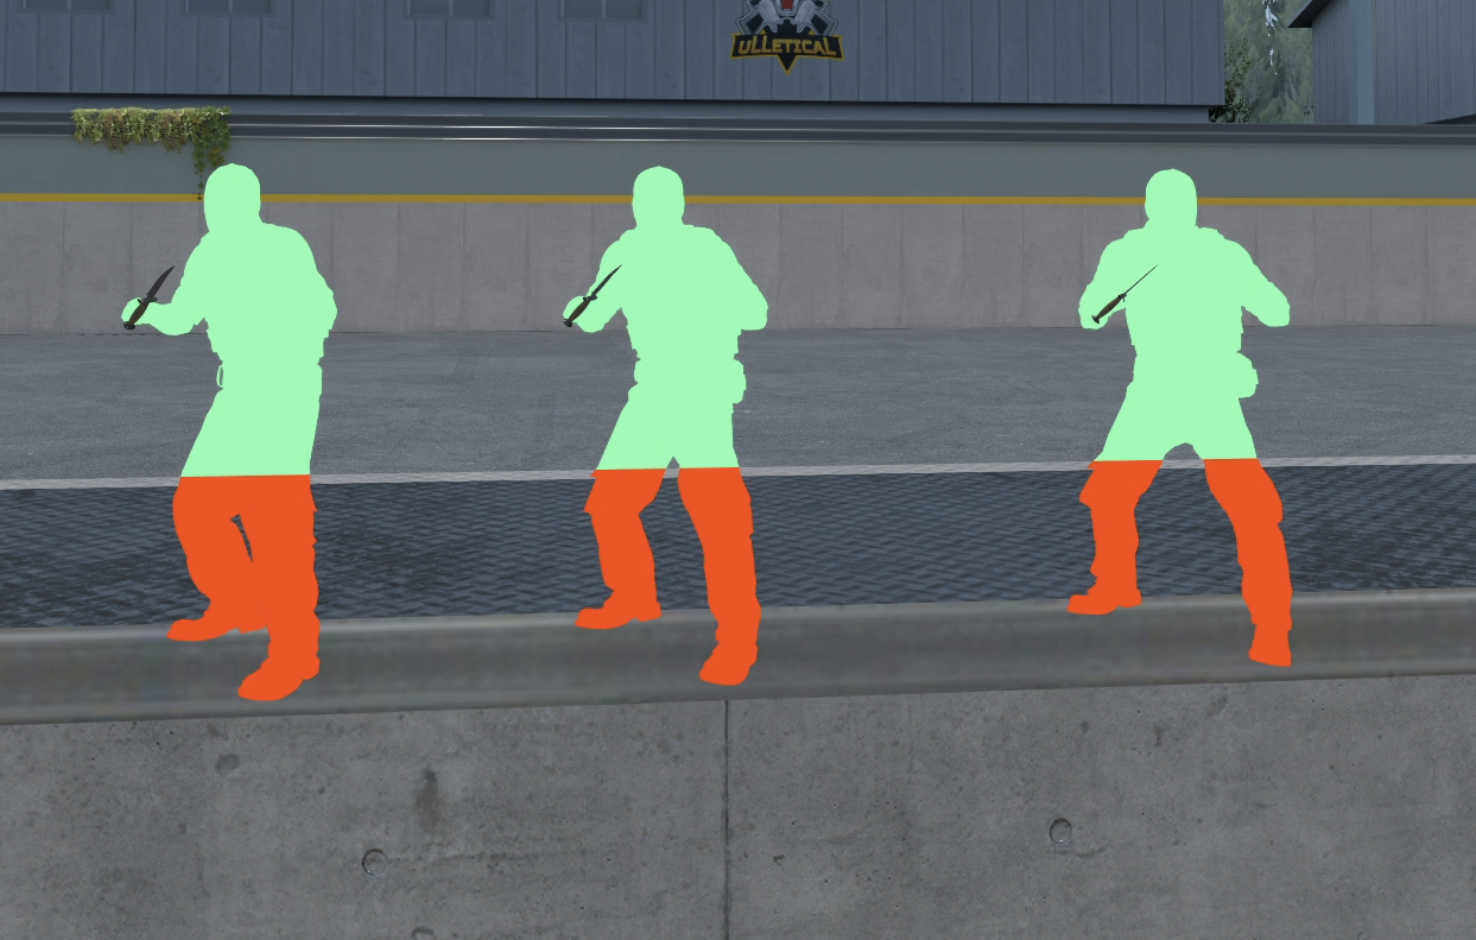
\includegraphics[width=0.33\textwidth,height=0.2\textheight]{images/chams/Screenshot 2025-04-28 at 03.03.27.png}%
        \hfill
        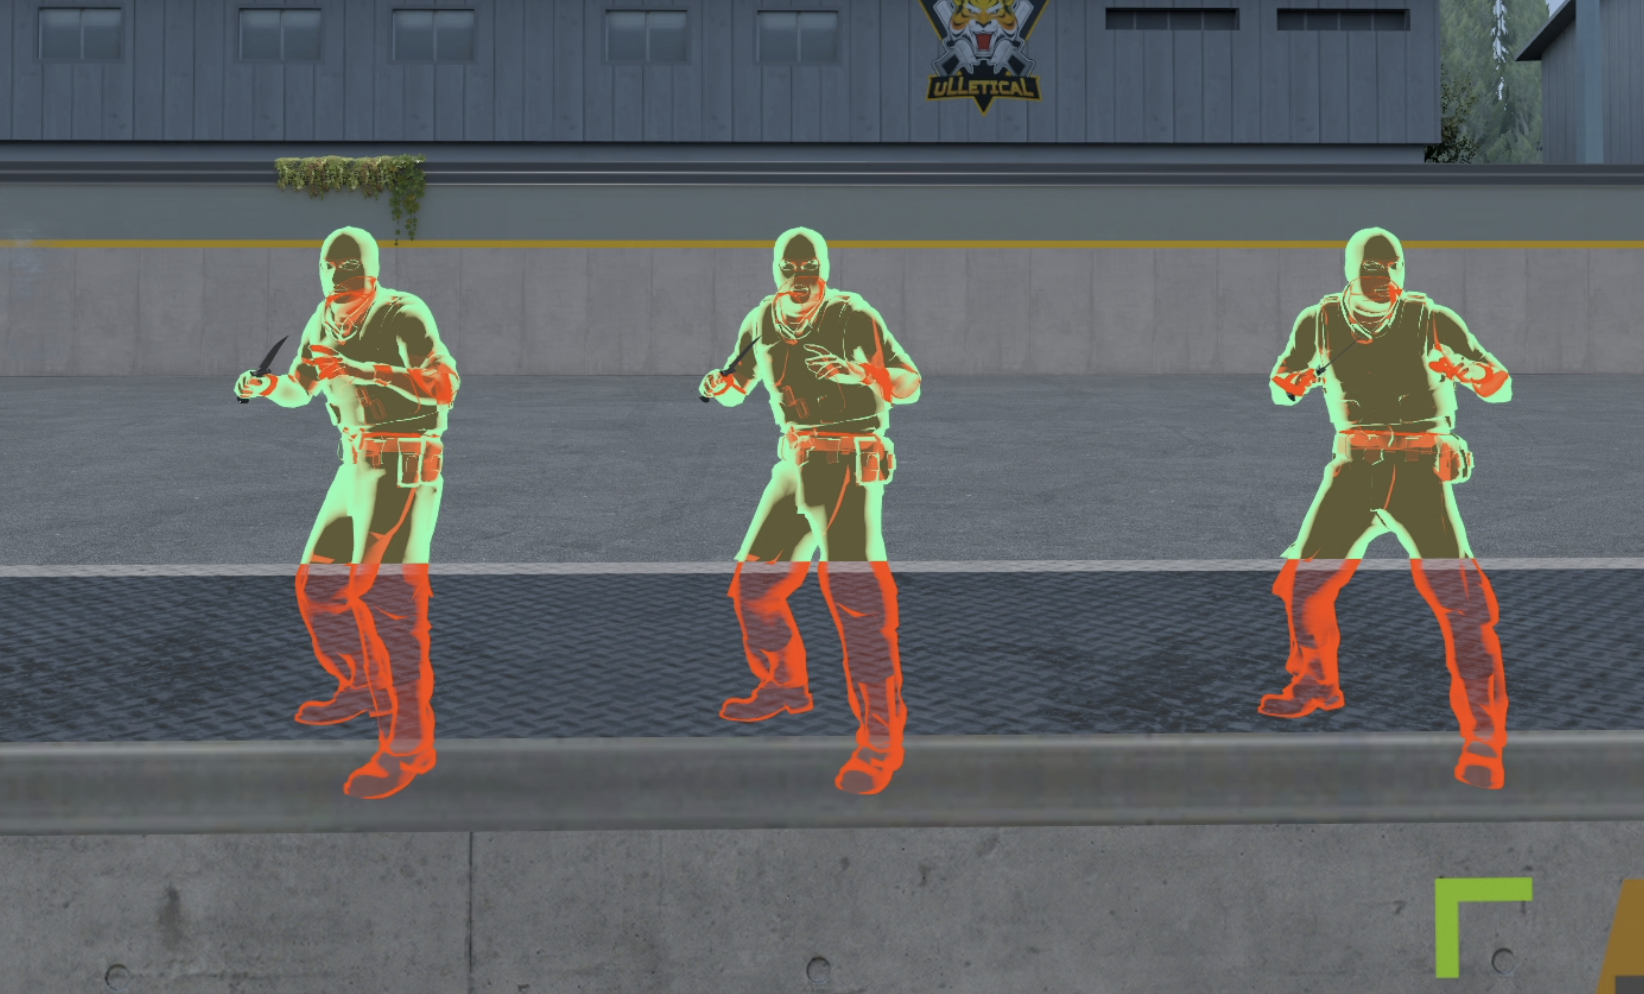
\includegraphics[width=0.33\textwidth,height=0.2\textheight]{images/chams/Screenshot 2025-04-28 at 03.04.21.png}%
        \hfill
        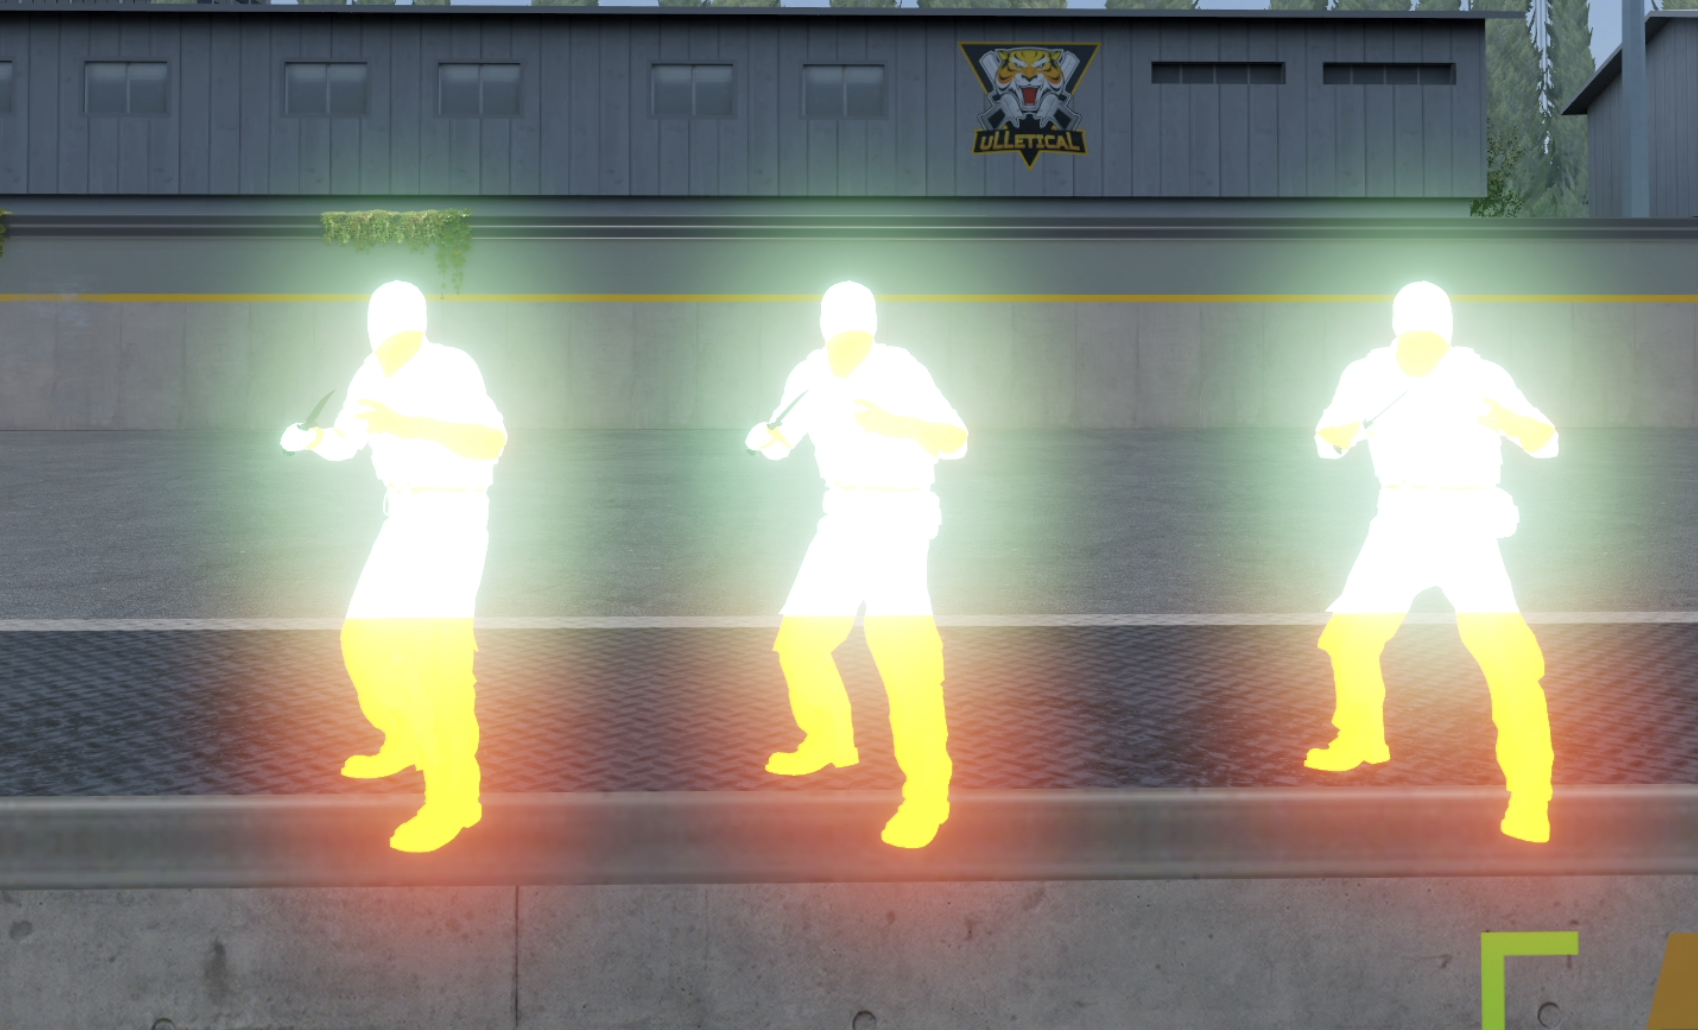
\includegraphics[width=0.33\textwidth,height=0.2\textheight]{images/chams/Screenshot 2025-04-28 at 03.04.58.png}%
    }

    \vspace{1.5pt} 

    \makebox[\textwidth][c]{%
        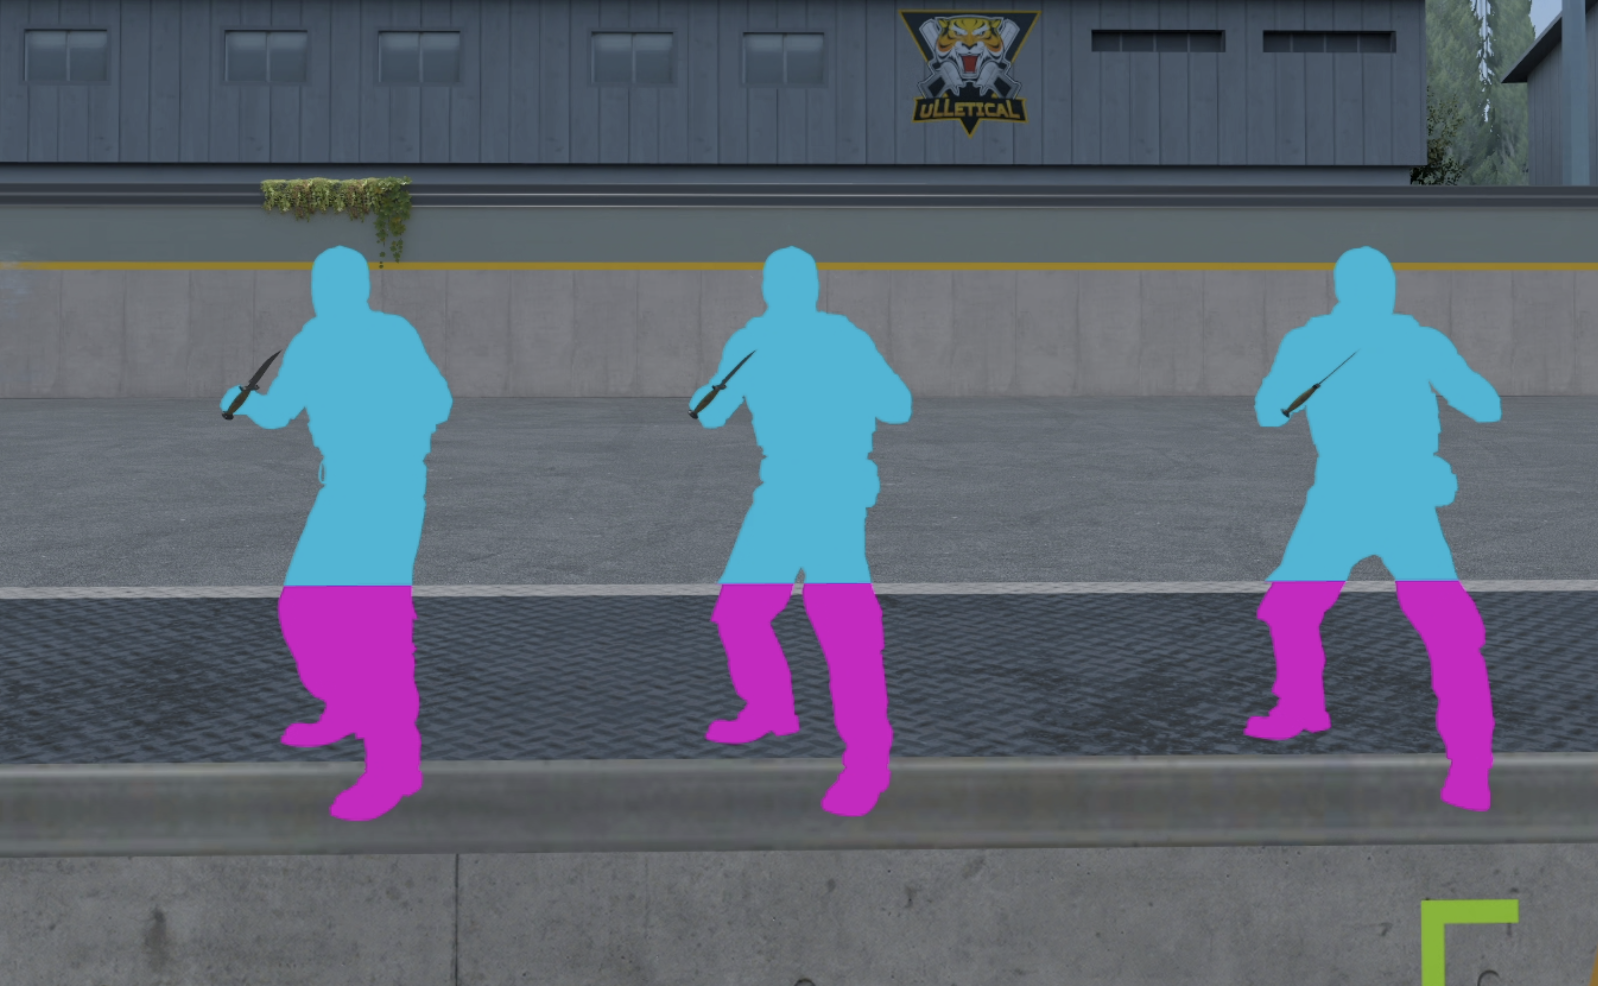
\includegraphics[width=0.33\textwidth,height=0.2\textheight]{images/chams/Screenshot 2025-04-28 at 03.05.36.png}%
        \hfill
        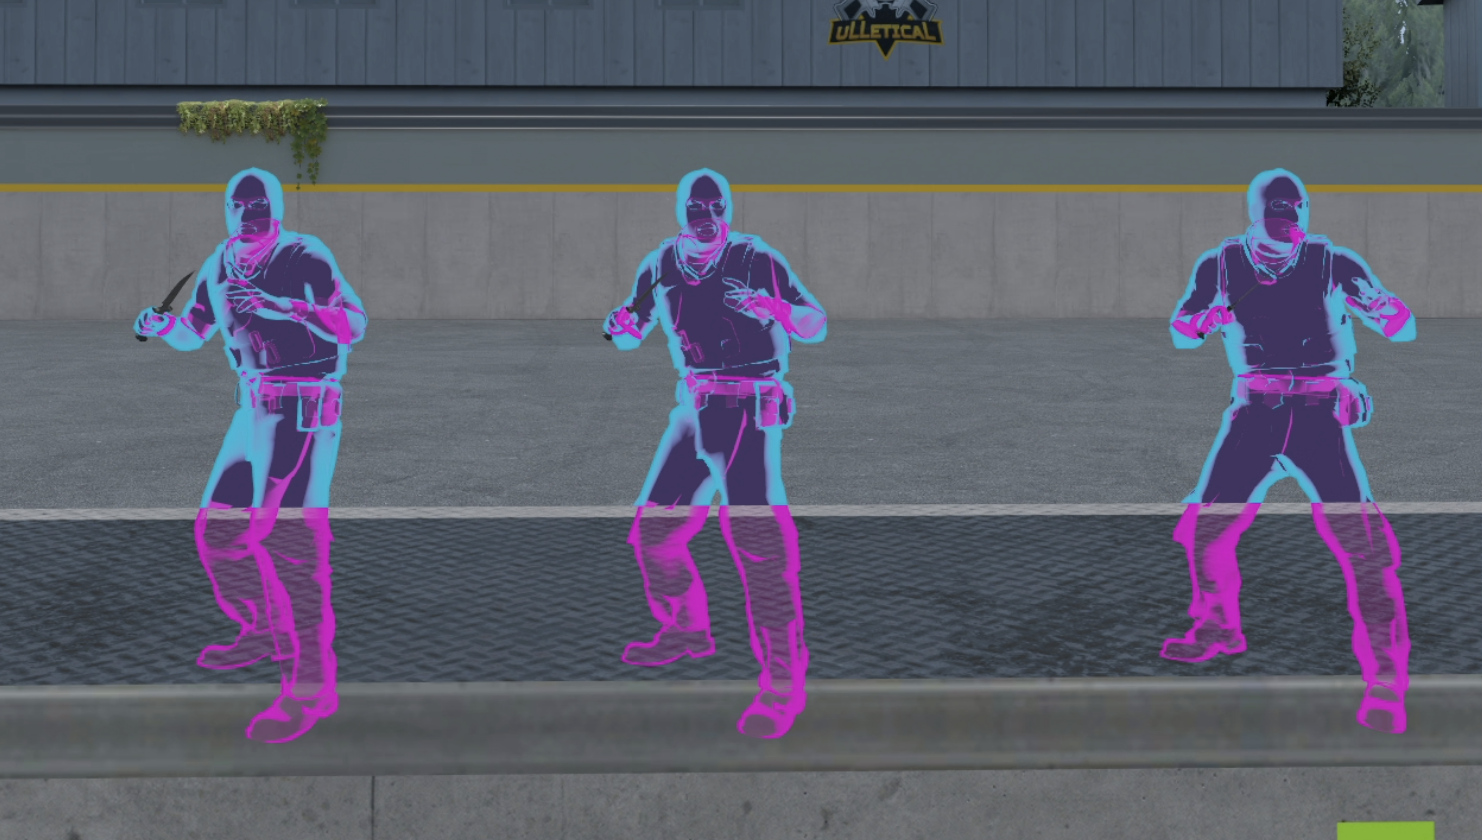
\includegraphics[width=0.33\textwidth,height=0.2\textheight]{images/chams/Screenshot 2025-04-28 at 03.05.50.png}%
        \hfill
        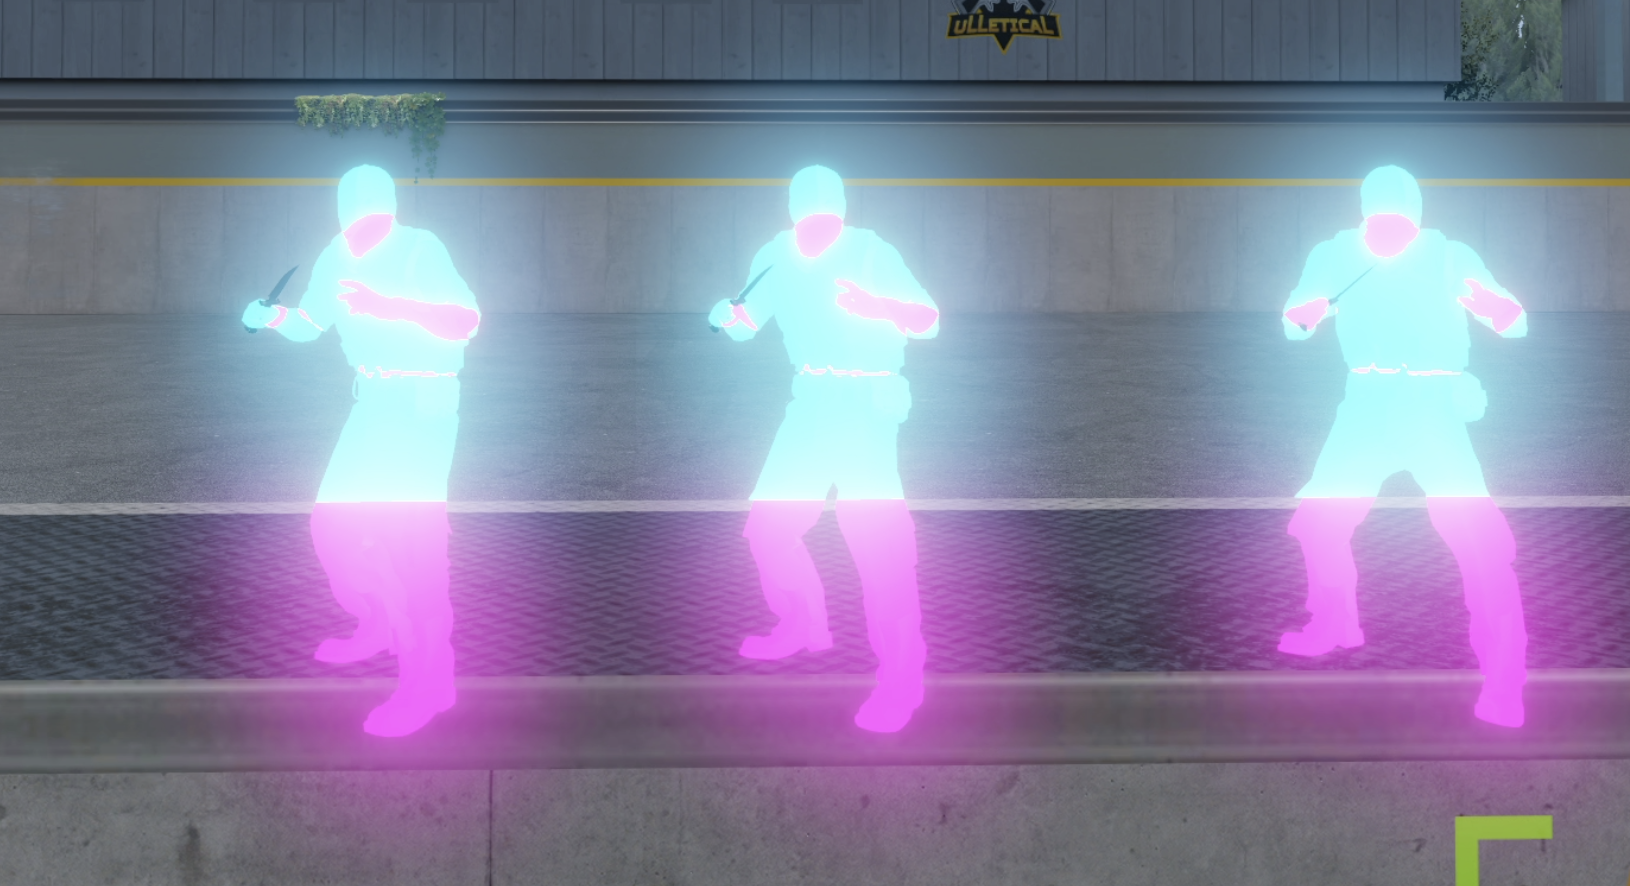
\includegraphics[width=0.33\textwidth,height=0.2\textheight]{images/chams/Screenshot 2025-04-28 at 03.06.35.png}%
    }

    \caption{Examples of custom Chams materials with visibility check enabled.}
\end{figure}

Before applying material overrides, it is possible to filter which game entities they affect. This allows for advanced customization where different materials can be applied not only to enemy player models, but also to the local player's model (arms and gloves) as well as their weapon. The following figure illustrates an example of this selective application:

\begin{figure}
    \centering
    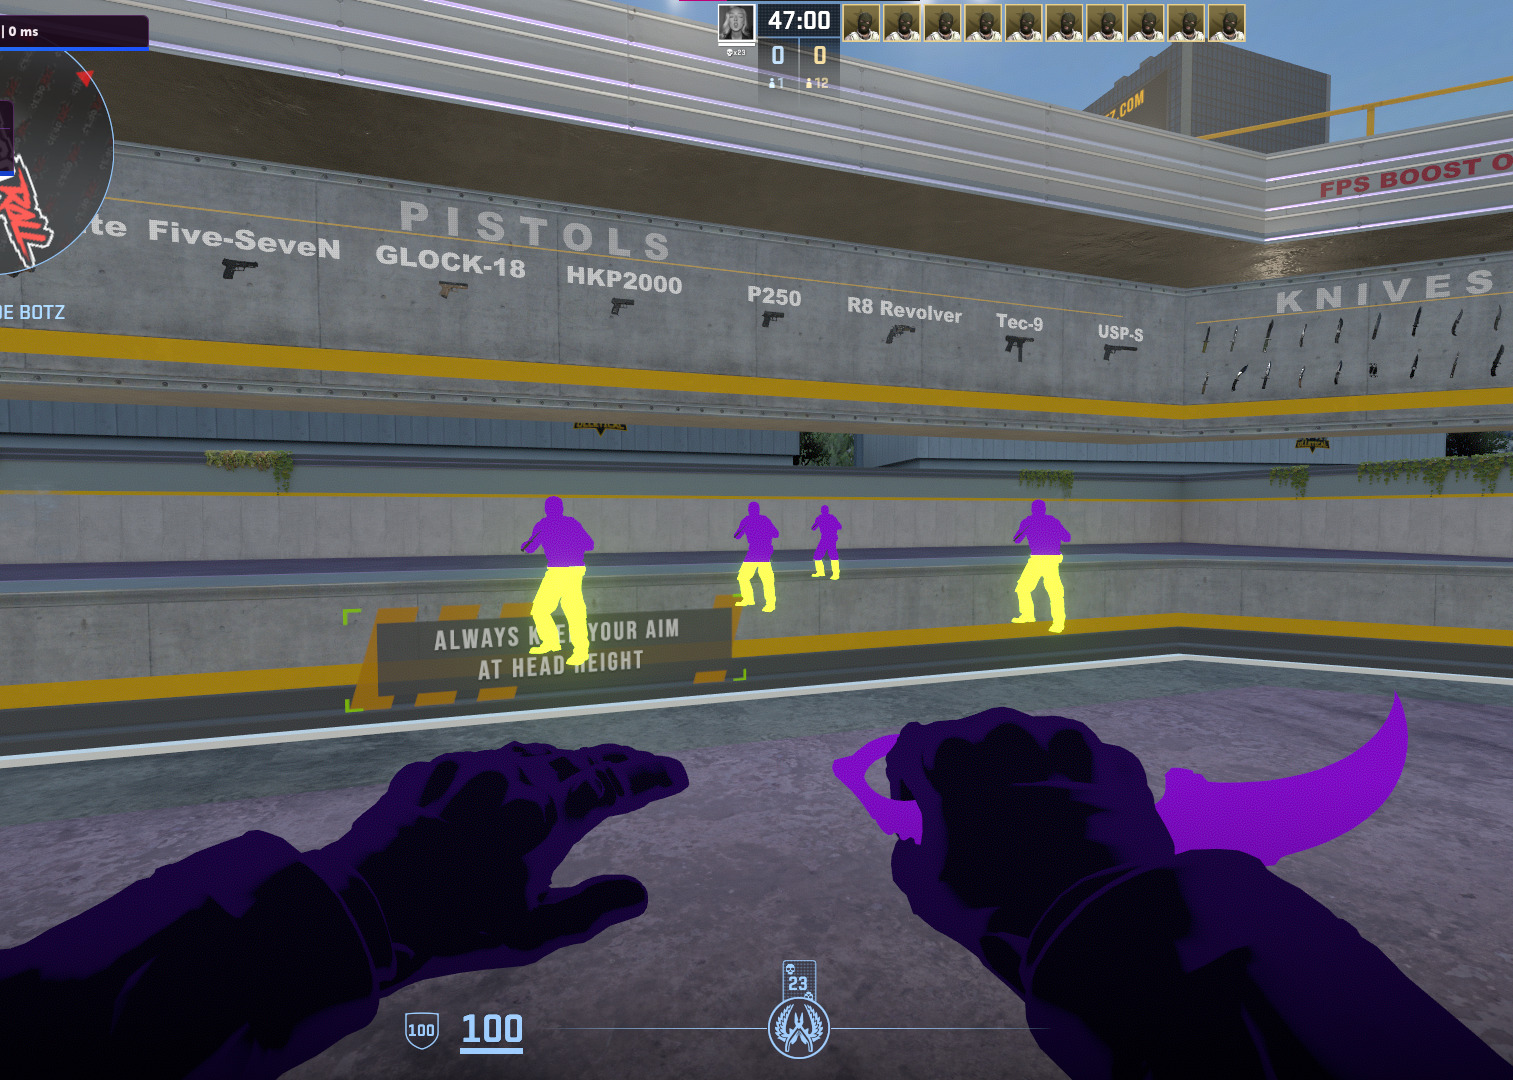
\includegraphics[width=1\linewidth]{images/visible_invisible_chams.png}
    \caption{Enter Caption}
    \label{fig:enter-label}
\end{figure}


\newpage


\section{Aimbot: Automated Aim to Enemy Players}


An aimbot is one of the most fundamental and widely recognized cheat functionalities in competitive first-person shooters. It automates the aiming process by computing the precise trajectory required to target an enemy, thereby bypassing human limitations in reaction time and accuracy. Developing an aimbot for \textit{Counter-Strike 2} (CS2) necessitates a comprehensive understanding of the game’s \textbf{entity system}, \textbf{coordinate transformations}, and \textbf{trigonometric principles} to ensure precise target alignment.

However, before implementing the aiming mechanism, it was crucial to first analyze how CS2 internally manages game entities. This understanding was essential since retrieving a player's position and calculating the required angles for the aimbot depend on accessing valid entity data. Without proper entity management, attempting to access a non-existent player could lead to dereferencing null pointers, resulting in critical errors or crashes.


\subsection{Computing Aiming Angles}

Achieving precise aiming in a three-dimensional environment like \textit{Counter-Strike 2} requires the aimbot to compute angular adjustments that align the player's crosshair with a target. Player orientation in CS2 is defined by three rotational angles:

\begin{itemize}
    \item \textbf{Pitch} (\(\theta\)): Controls vertical movement, determining how much the player looks up or down.
    \item \textbf{Yaw} (\(\phi\)): Governs horizontal movement, rotating the player's view left or right.
    \item \textbf{Roll} (\(\psi\)): Represents tilt along the forward axis but remains fixed at zero in CS2.
\end{itemize}

\begin{figure}[h!]
    \centering
    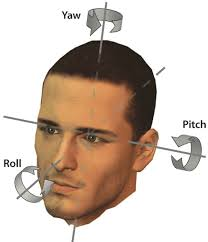
\includegraphics[width=0.78\linewidth]{images/image.png}
    \caption{Representation of Pitch, Yaw, and Roll in a 3D Space.}
    \label{fig:pitch_yaw_roll}
\end{figure}

While \textbf{pitch} and \textbf{yaw} dictate aiming direction in CS2, the \textbf{roll angle} remains fixed at zero. Unlike flight simulators or VR applications, where roll introduces an additional degree of freedom, CS2 enforces strict constraints that prevent camera tilting. Altering the roll angle would lead to an \textbf{impossible in-game state}, triggering \textbf{Valve Anti-Cheat (VAC)} detection and an automatic ban.



\subsubsection{Deriving the Direction Vector}

To accurately compute the aiming angles, the first step is to determine the enemy's position relative to the player's viewpoint. This process involves obtaining the player's position on the map, referred to as the \emph{foot position}, and then retrieving the camera position, which represents the player's \emph{eye position}. The eye position is the viewpoint from which the player perceives the game environment.

All positions are represented as three-dimensional vectors, \( \text{Vec3} \), consisting of three floating-point values: \( x, y, z \).

\subsubsection{Computing the Player’s Position}

The player's final position in the game world is obtained by adding the base position of the player to the camera offset:

\[
P_{\text{player}} = P_{\text{base}} + P_{\text{camera}}
\]

Where:
\begin{itemize}
    \item \( P_{\text{player}} \) is the final computed position of the player.
    \item \( P_{\text{base}} \) is the player's base position in the world.
    \item \( P_{\text{camera}} \) is the camera offset (view position).
\end{itemize}

\begin{figure}[h!]
    \centering
    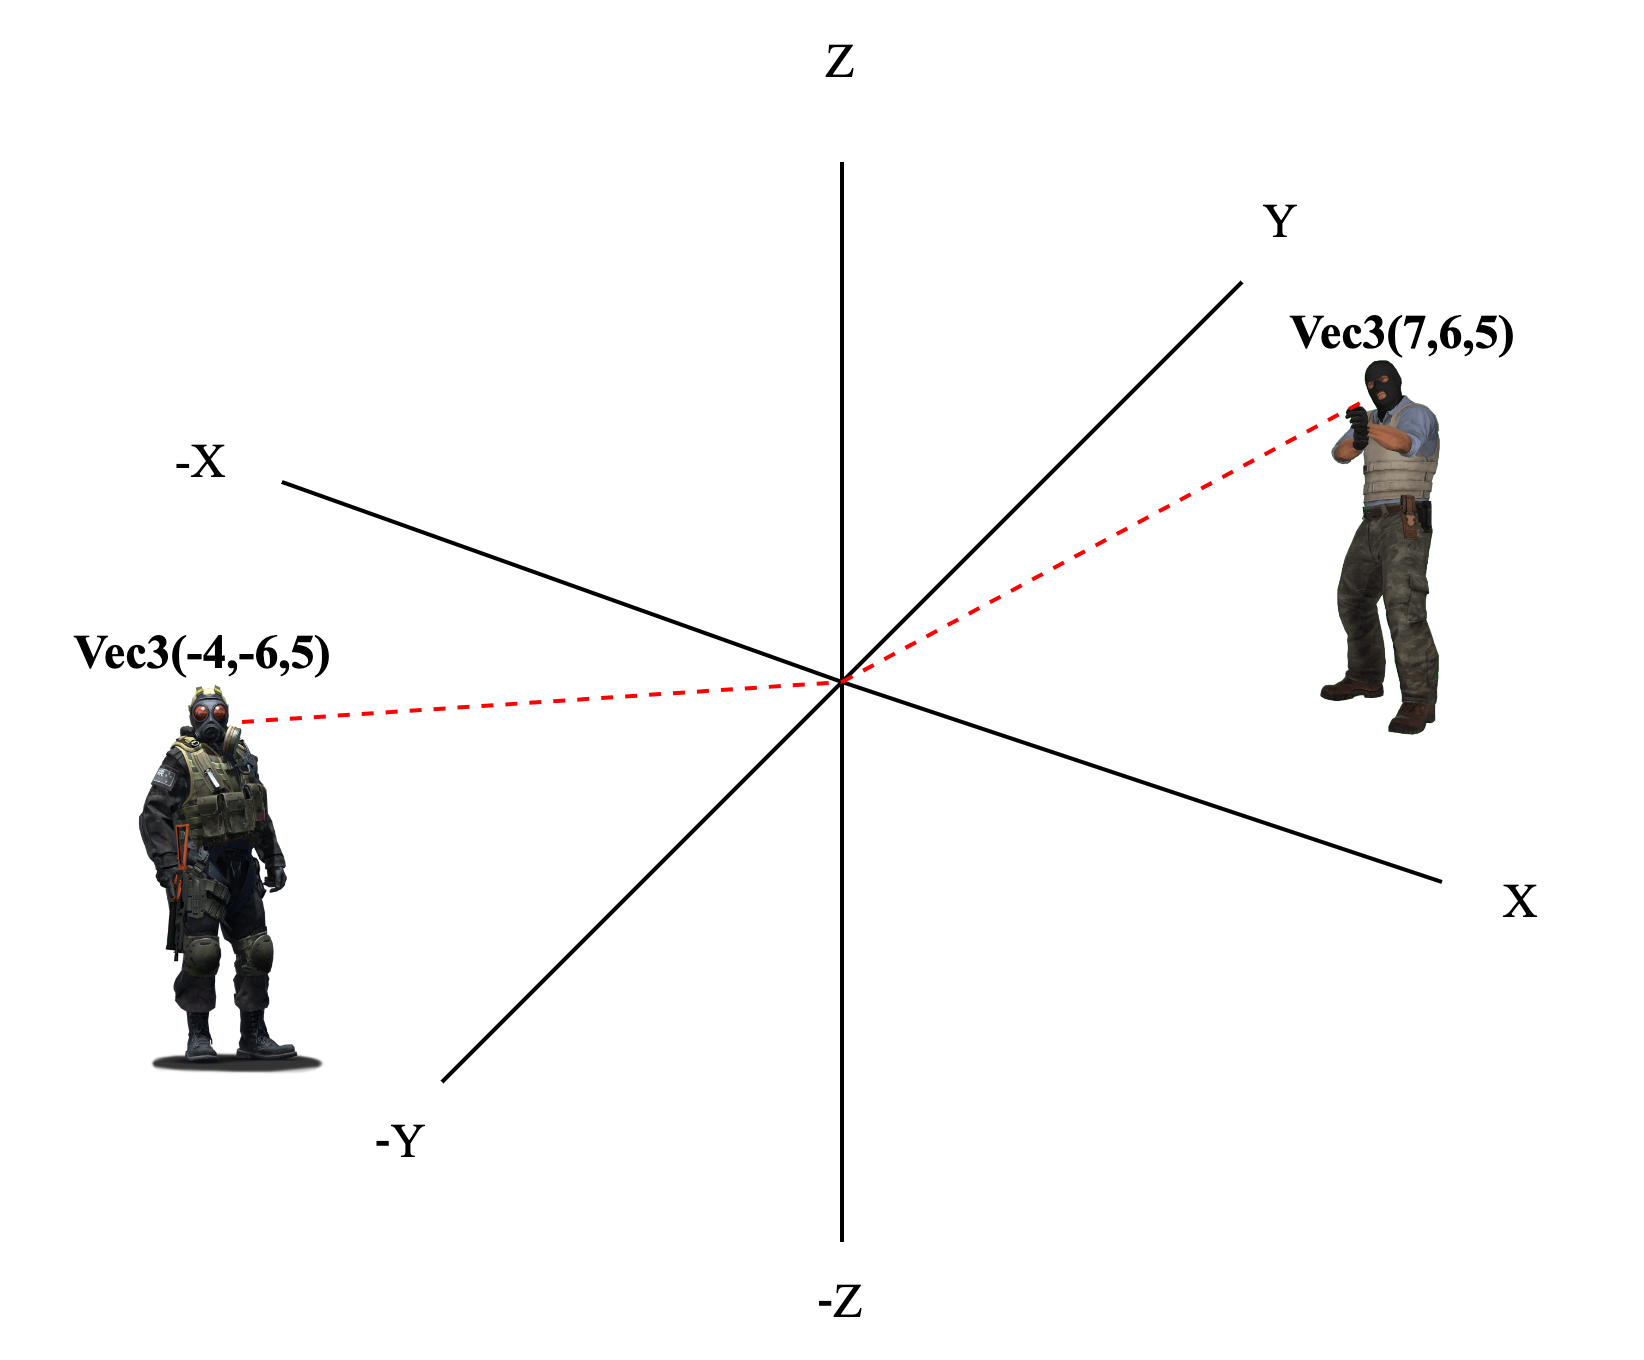
\includegraphics[width=0.78\linewidth]{images/Aimbot/Untitled Diagram.png}
    \caption{Representation of the player and enemy positions on the map.}
    \label{fig:player_enemy_positions}
\end{figure}


Expressed in vector form:

\[
\mathbf{P}_{\text{player}} =
\begin{bmatrix} 
    x_{\text{base}} \\ 
    y_{\text{base}} \\ 
    z_{\text{base}} 
\end{bmatrix} 
+ 
\begin{bmatrix} 
    x_{\text{camera}} \\ 
    y_{\text{camera}} \\ 
    z_{\text{camera}} 
\end{bmatrix}
\]


\subsubsection{Centering Coordinates on the Enemy}

To center the coordinate system on the enemy, we compute the relative position of the enemy with respect to the player by subtracting the player's position from the enemy's position:

\[
D = P_{\text{enemy}} - P_{\text{player}}
\]


\begin{figure}[h!]
    \centering
    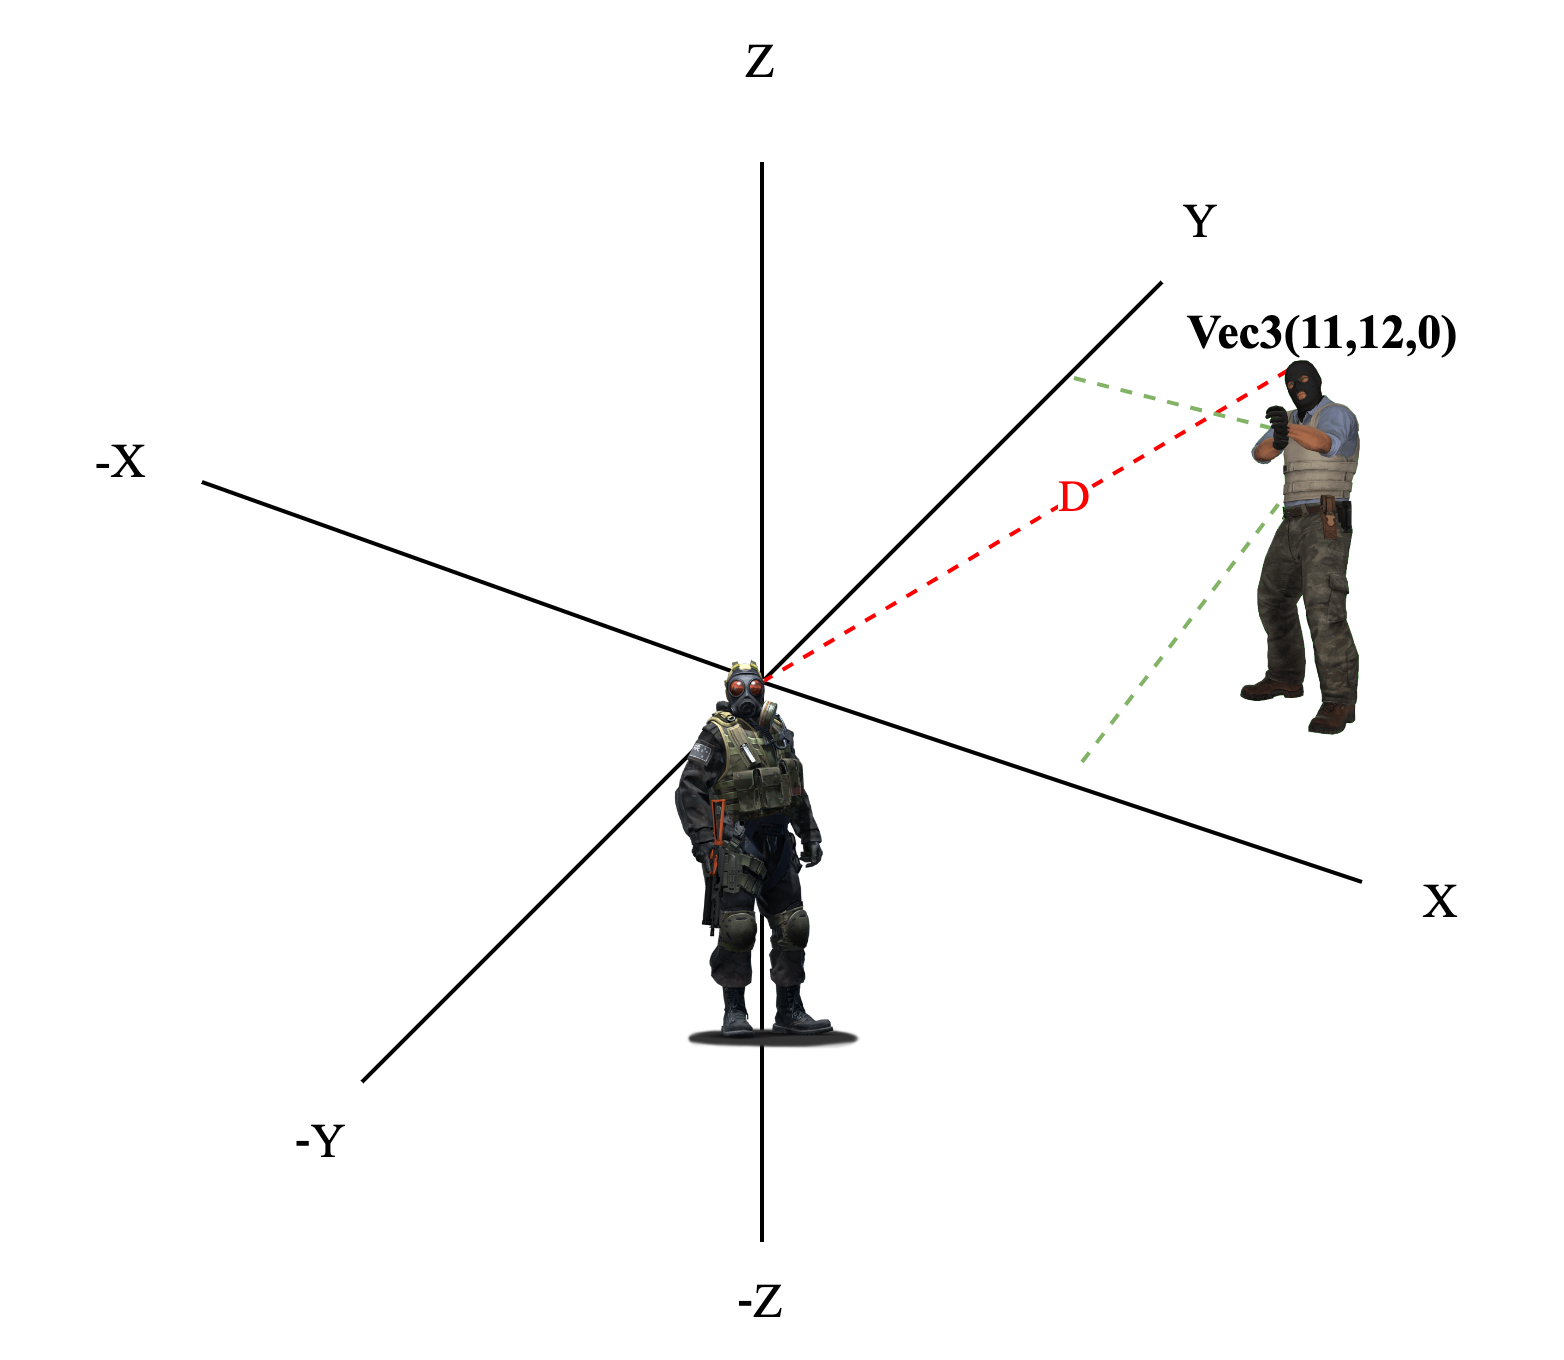
\includegraphics[width=0.78\linewidth]{images/Aimbot/Two.png}
    \caption{Original view with coordinate axes.}
    \label{fig:original_view}
\end{figure}


Expressed in vector form:

\[
\mathbf{D} =
\begin{bmatrix} 
    x_{\text{enemy}} - x_{\text{player}} \\ 
    y_{\text{enemy}} - y_{\text{player}} \\ 
    z_{\text{enemy}} - z_{\text{player}} 
\end{bmatrix}
\]

\subsection{Local Coordinate System and Angle Calculation}

As illustrated in Figure~\ref{fig:direction_vector}, all calculations take place in a local coordinate system where the player’s eye position serves as the \textbf{origin}. The computed direction vector \( D \), depicted by the blue line, serves as the foundation for determining the required pitch and yaw adjustments.

\begin{figure}[h!]
    \centering
    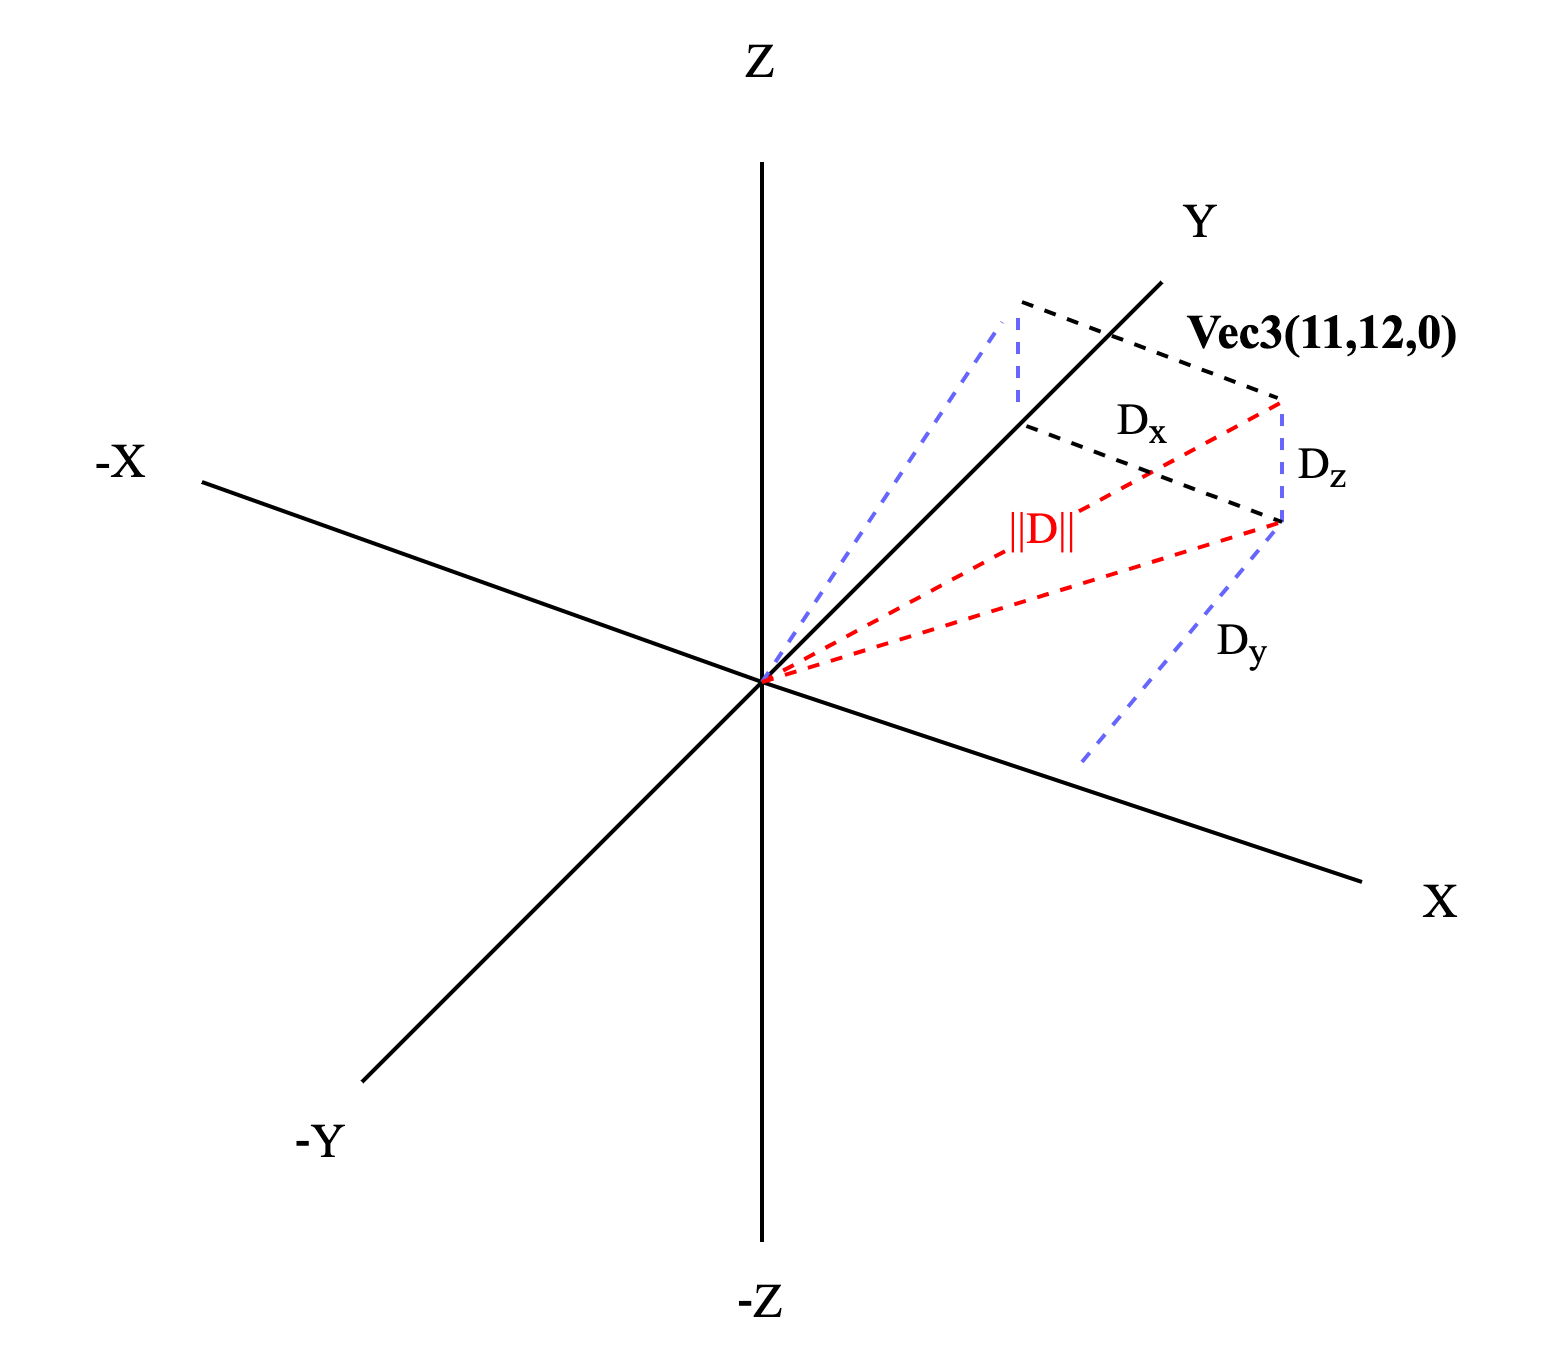
\includegraphics[width=0.75\linewidth]{images/Aimbot/Untitled Diagram(3).png}
    \caption{3D representation of the aiming direction vector.}
    \label{fig:direction_vector}
\end{figure}

This displacement vector is essential for calculating the angles necessary to adjust the player's aim. The yaw and pitch angles can be derived using trigonometric functions, which will be explored in the next section.


\subsubsection{Mathematical Computation of Aiming Angles}

Once the direction vector is obtained, the aimbot calculates the required \textbf{pitch} and \textbf{yaw} angles to align the player's crosshair with the target.

\paragraph{\textbf{Pitch Calculation} (\(\theta\))}  
The vertical adjustment necessary to match the enemy’s head height is determined by:

\[
\theta = \arcsin \left( \frac{D_z}{||D||} \right)
\]

where:

\[
||D|| = \sqrt{D_x^2 + D_y^2 + D_z^2}
\]

The \textbf{pitch} angle (\(\theta\)) is limited between \textit{\textbf{-90° and 90°}}, which corresponds to looking straight up or straight down.

\paragraph{\textbf{Yaw Calculation} (\(\phi\))}  
The horizontal adjustment required to rotate the player towards the enemy is calculated as:

\[
\phi = \arctan2(D_y, D_x)
\]

The function \(\arctan2(D_y, D_x)\) is used instead of \(\arctan(D_y / D_x)\) because it correctly determines the quadrant of the angle and prevents division errors when \( D_x = 0 \). The \textbf{yaw} angle (\(\phi\)) spans from \textit{\textbf{-180° to 180°}}, covering all possible directions.

\paragraph{\textbf{Angle Conversion:}}  
Since CS2 operates in degrees, a conversion from radians is necessary:

\[
\theta_{\text{degrees}} = \theta \times \frac{180}{\pi}, \quad
\phi_{\text{degrees}} = \phi \times \frac{180}{\pi}
\]



\subsection{Overwriting Player View Angles}

Once the aiming angles are computed, they must be applied to the player’s in-game camera. This is achieved by hooking into the game’s function responsible for setting view angles:

\begin{lstlisting}[style=cppstyle, caption={Overwriting Player View Angles}]
typedef void (__fastcall *SetViewAnglesFunction)(__int64 *a1, __int64 a2, Vec3 a3);
\end{lstlisting}

This function takes the following parameters:
\begin{itemize}
    \item A pointer to the player’s entity.
    \item An auxiliary parameter related to camera state.
    \item A vector \texttt{a3} containing the new pitch and yaw angles.
\end{itemize}

By injecting the computed angles into this function, the aimbot effectively reorients the player's view towards the target, ensuring near-instant alignment with minimal latency.

\subsection{Smoothing for Stealth}

To avoid detection by VAC, direct modifications to view angles are interpolated over multiple frames using a \textbf{smoothing algorithm}:

\[
\theta_{\text{new}} = \theta_{\text{current}} + \frac{(\theta_{\text{target}} - \theta_{\text{current}})}{S}
\]

\[
\phi_{\text{new}} = \phi_{\text{current}} + \frac{(\phi_{\text{target}} - \phi_{\text{current}})}{S}
\]

where \( S \) is the smoothing factor controlling transition speed. A larger smoothing value results in slower, human-like movements, significantly reducing the likelihood of detection.

By implementing smooth interpolation rather than instantaneously snapping to a target, the aimbot mimics natural aiming behaviors, thereby remaining undetected by VAC while maintaining effectiveness.


\section{Bone Calculation: Extracting and Rendering Player Skeletons}

In this section, we describe how we extracted, visualized, and connected the bone structures used to animate player models in \textit{Counter-Strike 2}. These bones are essential for accurately representing player movement and orientation, and form the foundation for many ESP and aimbot features.

\subsection{Extracting Bone Data from Player Entities}

Each \texttt{PlayerPawn} entity in CS2 contains an internal memory structure that holds an array of bones. These bones represent all animation joints of the player model, from the pelvis and spine to the fingertips and eyes.

Through reverse engineering and memory analysis, we identified the layout of each bone entry in memory. Each bone follows the following structure:

\begin{lstlisting}[style=cppstyle, caption={Bone Memory Structure}]
class BoneData_t {
public:
    Vec3 vecPosition;           // 3D world-space position
    float flScale;              // Scale factor for animation
    Vector4D_t vecRotation;     // Rotation quaternion
};
\end{lstlisting}

This structure allows us to read the world-space position of each bone, which is later projected to screen coordinates for overlay rendering.

To access these bones, we enumerated all relevant bone indices used by terrorist player models. After extensive experimentation, we constructed a detailed enumeration mapping each bone to its corresponding index in memory. The following snippet presents a partial view of the enumeration:

\begin{lstlisting}[style=cppstyle, caption={Terrorist Bone Index Enumeration}]
namespace terroristBones {
    enum tBones : DWORD {
        pelvis = 0,
        spine_0 = 1,
        spine_1 = 2,
        spine_2 = 3,
        spine_3 = 4,
        neck_0 = 5,
        head_0 = 6,
        // ... continued through to:
    };
}
\end{lstlisting}

This enumeration enables us to reference bones by name rather than raw index values, improving both readability and maintainability in our codebase.

\subsection{Visualizing Bone Indices on the Player Model}

After accessing the bone data, we developed a visualization tool to display each bone's index directly on the screen using our external overlay. This feature allows real-time debugging and inspection of the full bone structure.

\begin{figure}[h!]
    \centering
    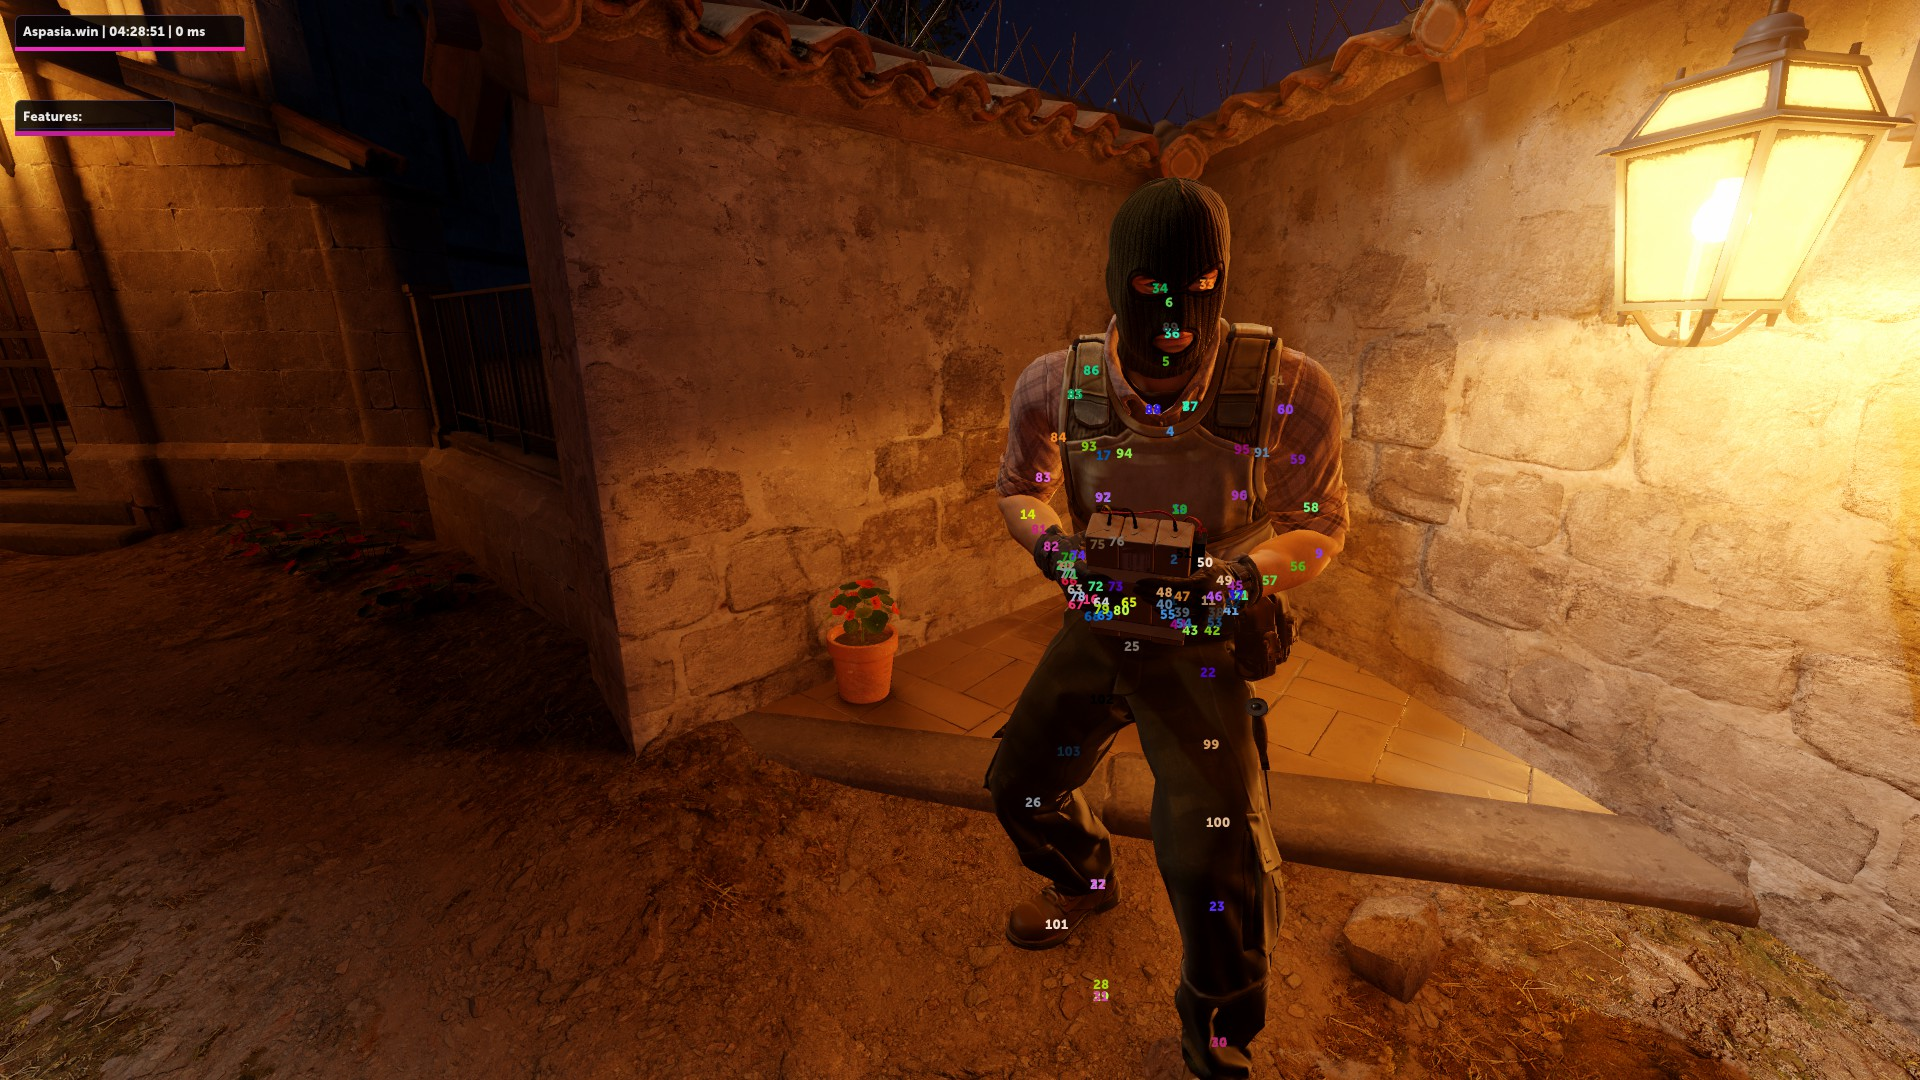
\includegraphics[width=0.95\linewidth]{images/Bones/730_22.jpg}
    \caption{Visualizing all bone indices rendered over the player model.}
    \label{fig:bone_debug}
\end{figure}



\begin{lstlisting}[style=cppstyle, caption={Displaying Bone Indices On-Screen}]
void RenderPlayerBones(C_PlayerPawn* player) {
    if (player == GetLocalPlayer()) return;

    for (int bone = terroristBones::pelvis; bone <= terroristBones::leg_upper_r_twist1; ++bone) {
        Vec3 worldPos = player->GetBone(bone)->vecPosition;
        Vec2 screenPos;

        if (!WorldToScreen(worldPos, screenPos)) continue;

        ImU32 color = IM_COL32((bone * 15) % 255, (bone * 35) % 255, (bone * 55) % 255, 255);
        DrawText(screenPos, std::to_string(bone).c_str(), color);
    }
}
\end{lstlisting}



This system projects each bone’s 3D position into 2D screen-space using the current game view matrix and renders its numeric index in a unique color. This was key for mapping bones during animation and ensuring accuracy in further rendering steps.

\subsection{Rendering a Connected Skeleton}

To enhance clarity and provide a meaningful representation of player posture, we implemented a simplified skeleton overlay. This system connects key bones with lines, forming a real-time stick-figure representation of the player’s body.

\begin{lstlisting}[style=cppstyle, caption={Drawing a Simplified Player Skeleton}]
void RenderSkeleton(C_PlayerPawn* player) {
    if (!player || player == GetLocalPlayer()) return;

    std::unordered_map<const char*, ImVec2> screenPos;
    for (auto& [name, index] : bones) {
        Vec3 world = player->GetBone(index)->vecPosition;
        Vec2 screen;
        if (WorldToScreen(world, screen)) {
            screenPos[name] = ImVec2(screen.x, screen.y);
        }
    }

    std::vector<std::pair<const char*, const char*>> links = {
        {"head", "neck"}, {"neck", "torso"}, {"torso", "pelvis"},
        {"torso", "left_clavicle"}, {"left_clavicle", "left_upper_arm"},
        {"left_upper_arm", "left_lower_arm"}, {"left_lower_arm", "left_hand"},
        . . .
        {"right_upper_leg", "right_lower_leg"}, {"right_lower_leg", "right_foot"}
    };

    for (auto& [a, b] : links) {
        if (screenPos.count(a) && screenPos.count(b)) {
            DrawLine(screenPos[a], screenPos[b], IM_COL32(255, 255, 255, 255), 2.0f);
        }
    }
}

\end{lstlisting}

This skeleton representation provides a clean and intuitive view of player pose and animation, aiding not only in cheat visualization but also in development of features such as aim prediction, hitbox tracing, and movement recognition.

\begin{figure}[h!]
    \centering
    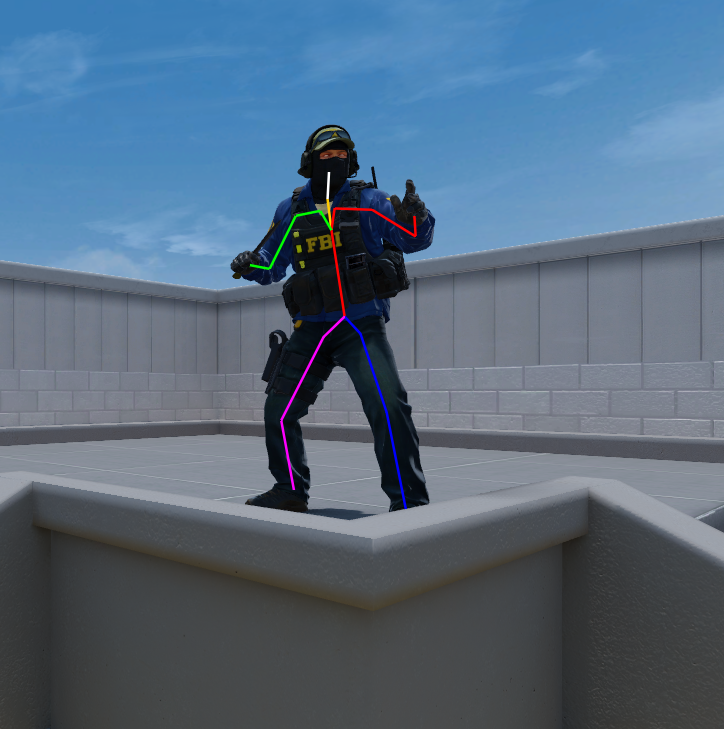
\includegraphics[width=0.8\linewidth]{images/imagen.png}
    \caption{Simplified player skeleton rendered using bone connections.}
    \label{fig:skeleton_overlay}
\end{figure}


\begin{figure}[H]
    \centering
    % Primera fila de 3 imágenes
    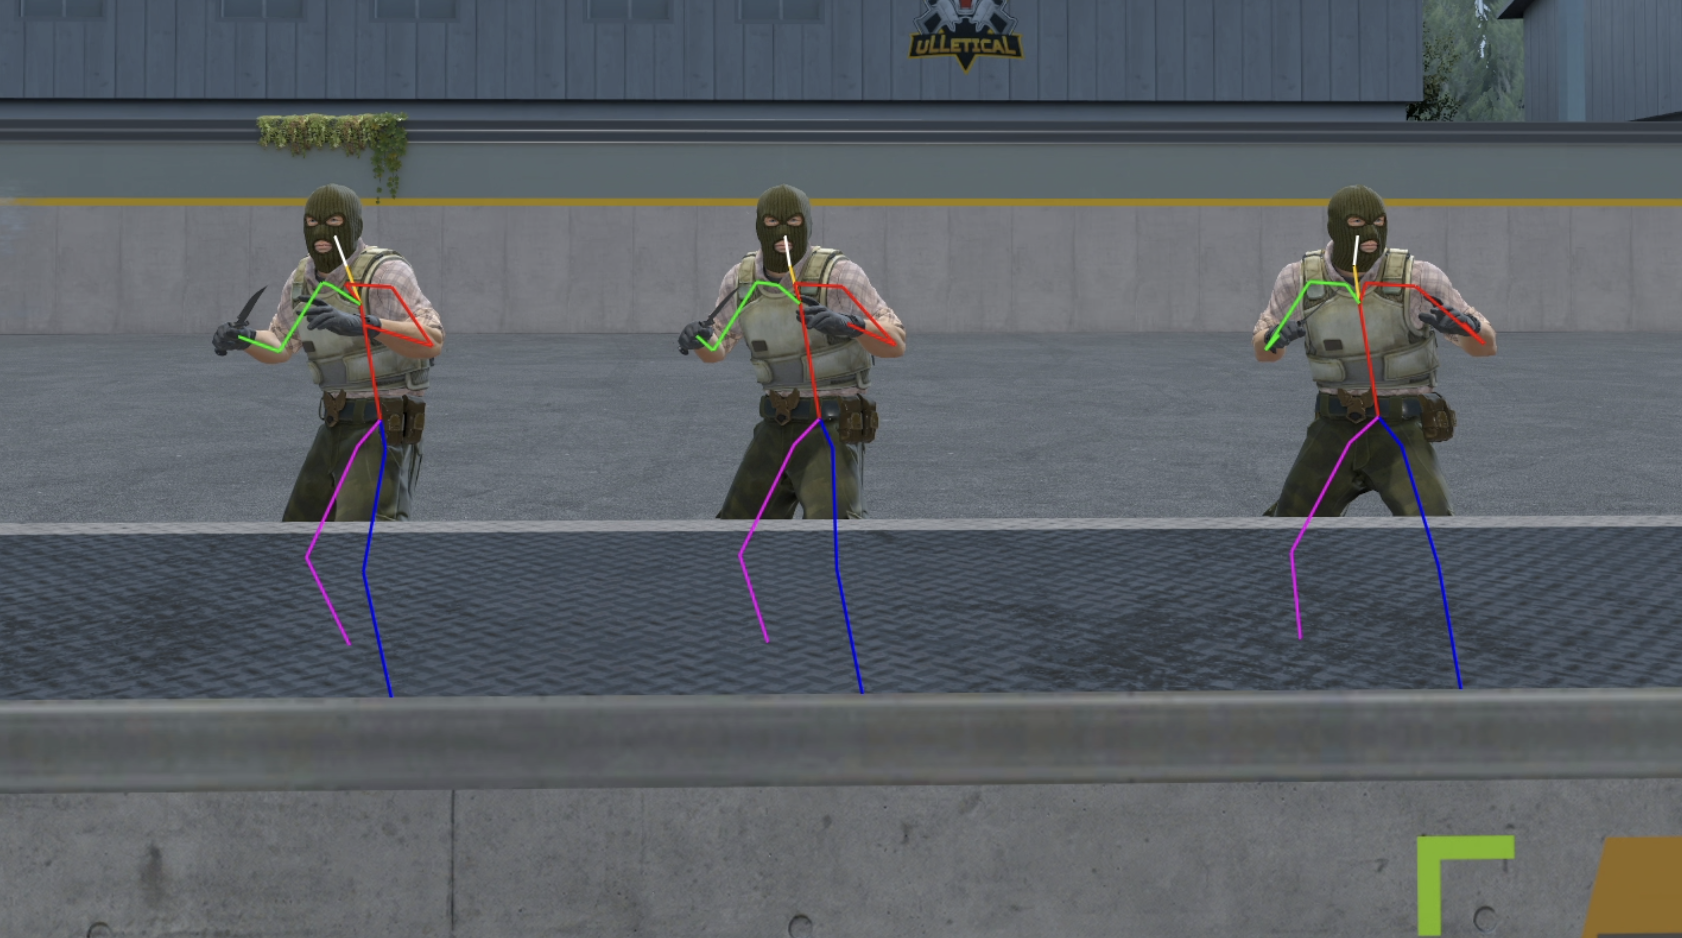
\includegraphics[width=0.33\textwidth,height=0.23\textheight]{images/chams/Screenshot 2025-04-28 at 03.19.49.png}\hspace{1pt}%
    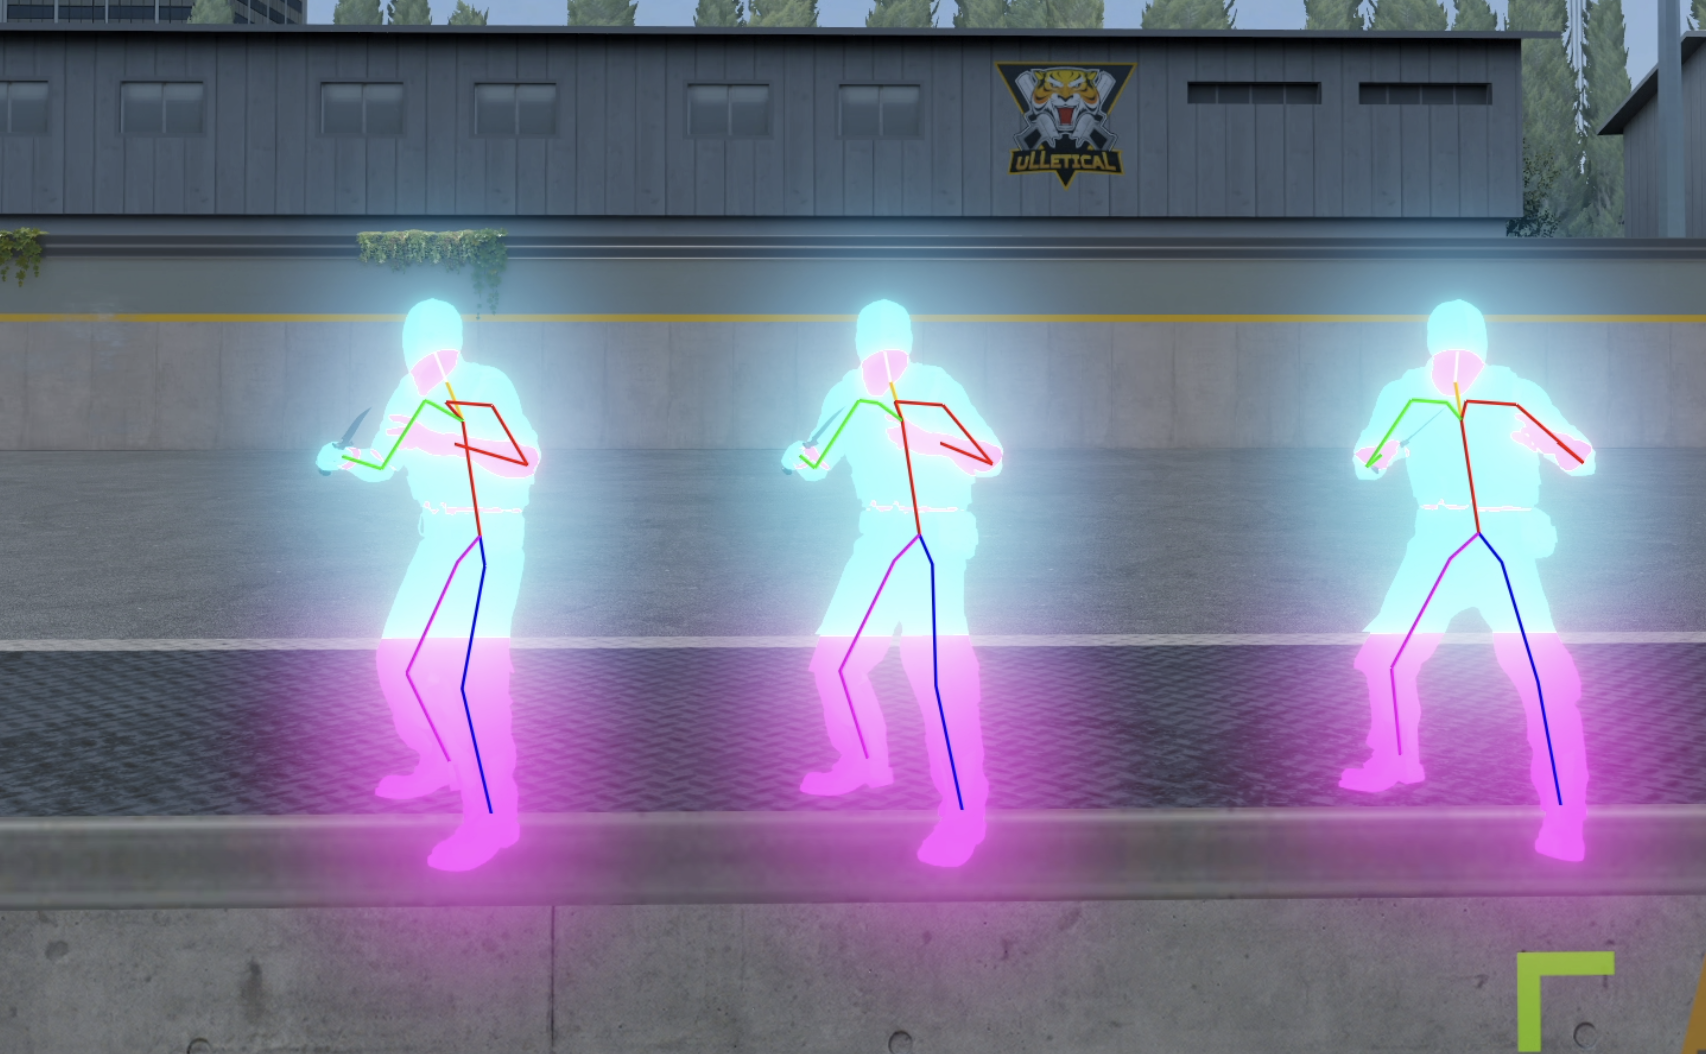
\includegraphics[width=0.33\textwidth,height=0.23\textheight]{images/chams/Screenshot 2025-04-28 at 03.20.26.png}\hspace{1pt}%
    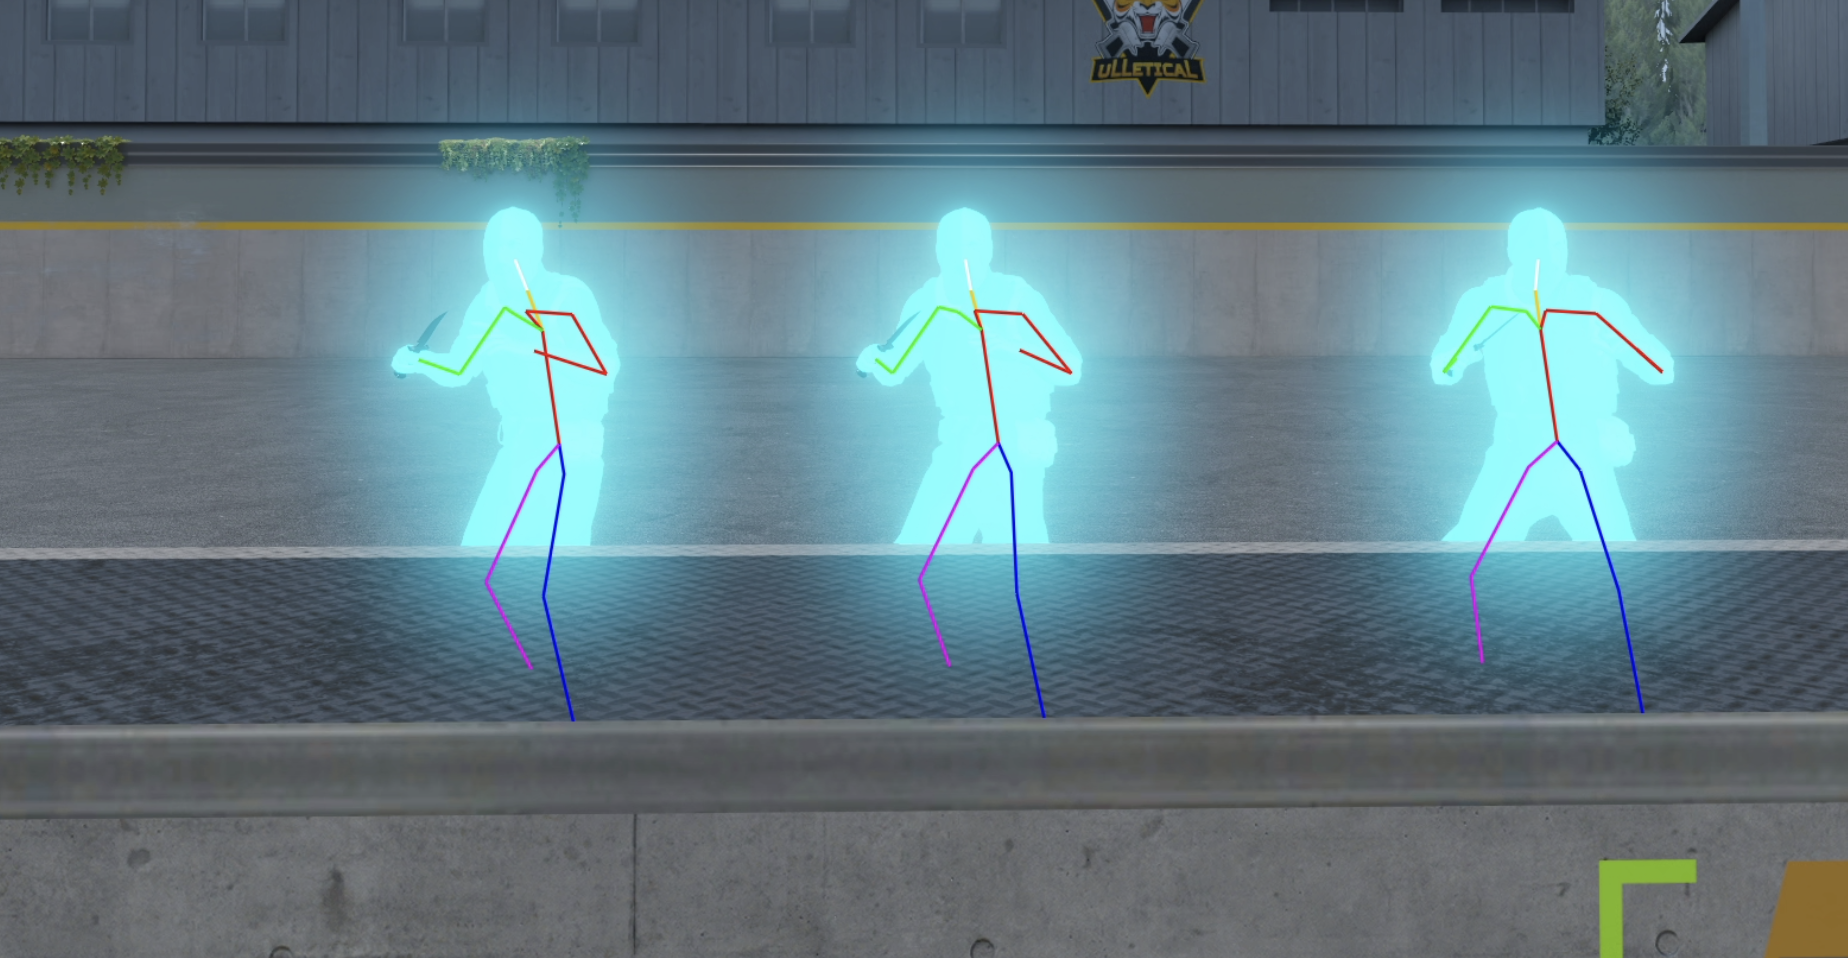
\includegraphics[width=0.33\textwidth,height=0.23\textheight]{images/chams/Screenshot 2025-04-28 at 03.20.41.png}\\[1pt]
    % Segunda fila de 3 imágen3es
    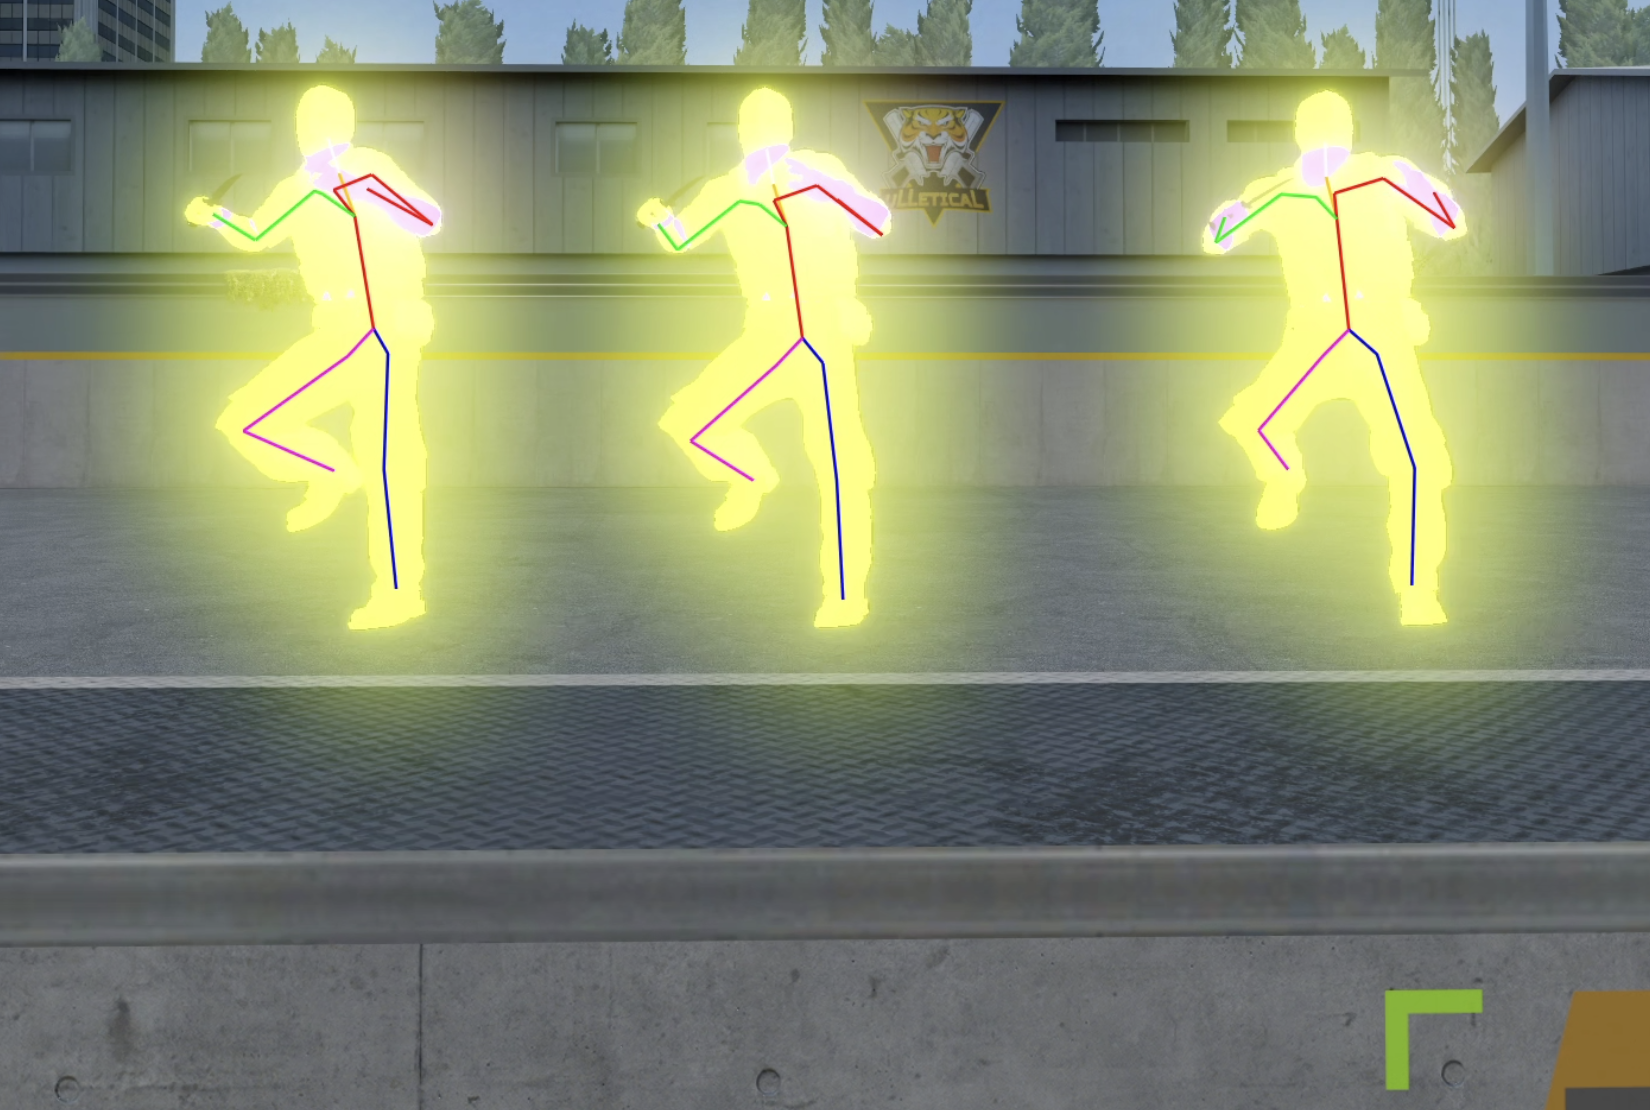
\includegraphics[width=0.33\textwidth,height=0.23\textheight]{images/chams/Screenshot 2025-04-28 at 03.21.36.png}\hspace{1pt}%
    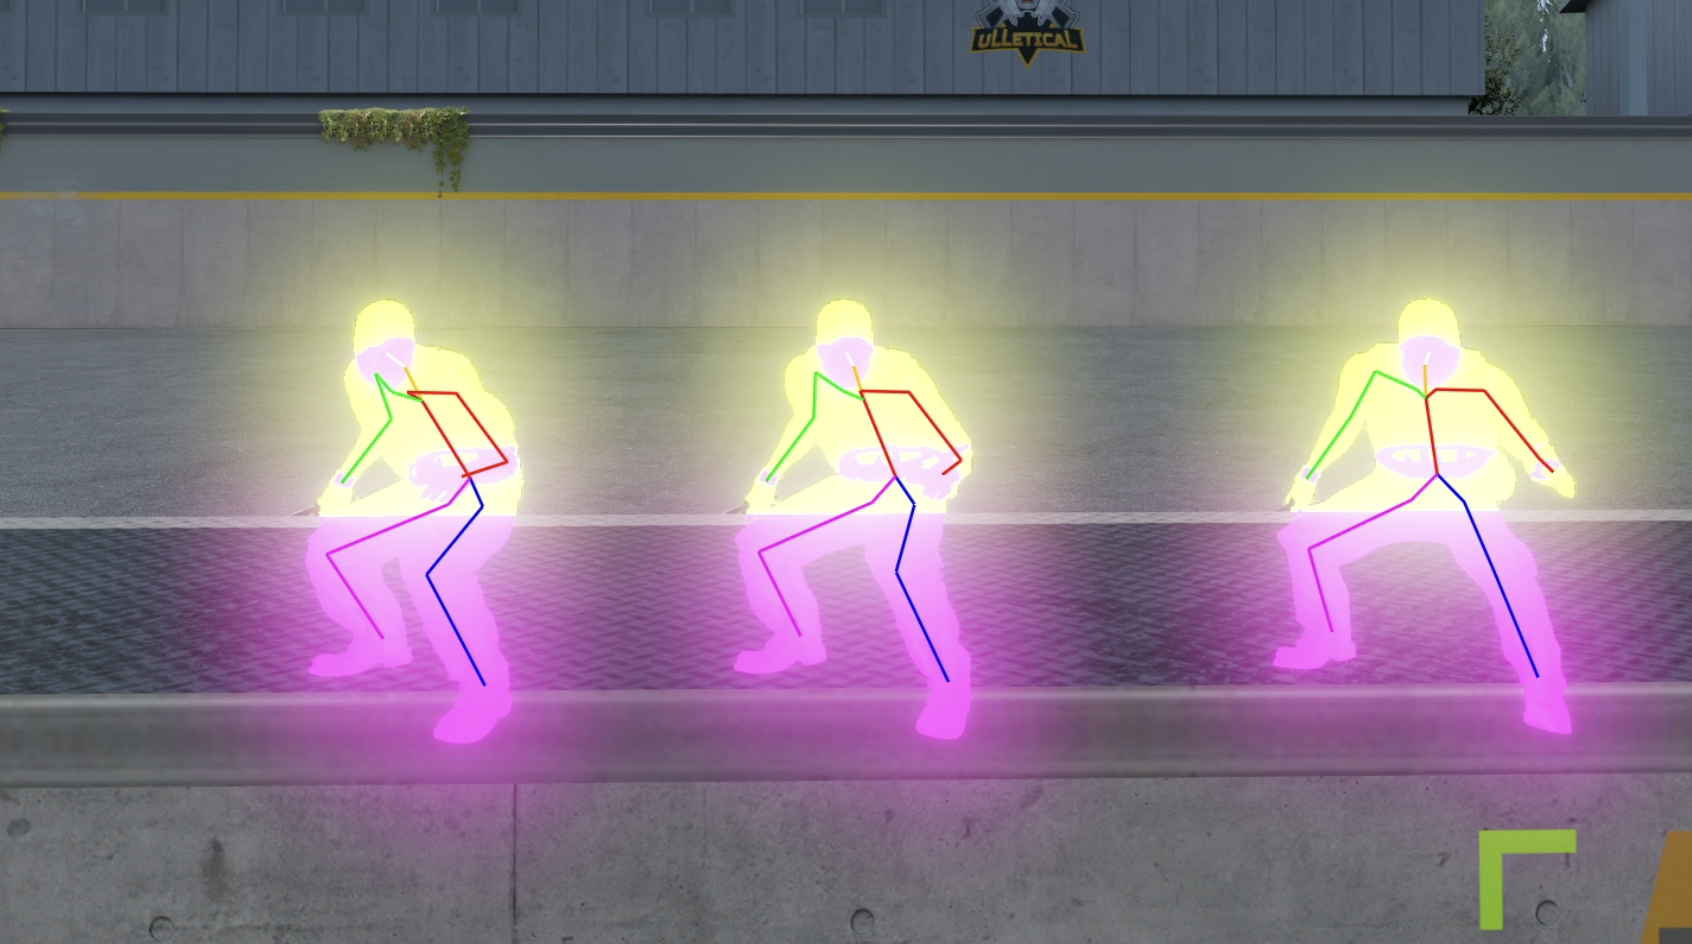
\includegraphics[width=0.33\textwidth,height=0.23\textheight]{images/chams/Screenshot 2025-04-28 at 03.22.09.png}\hspace{1pt}%
    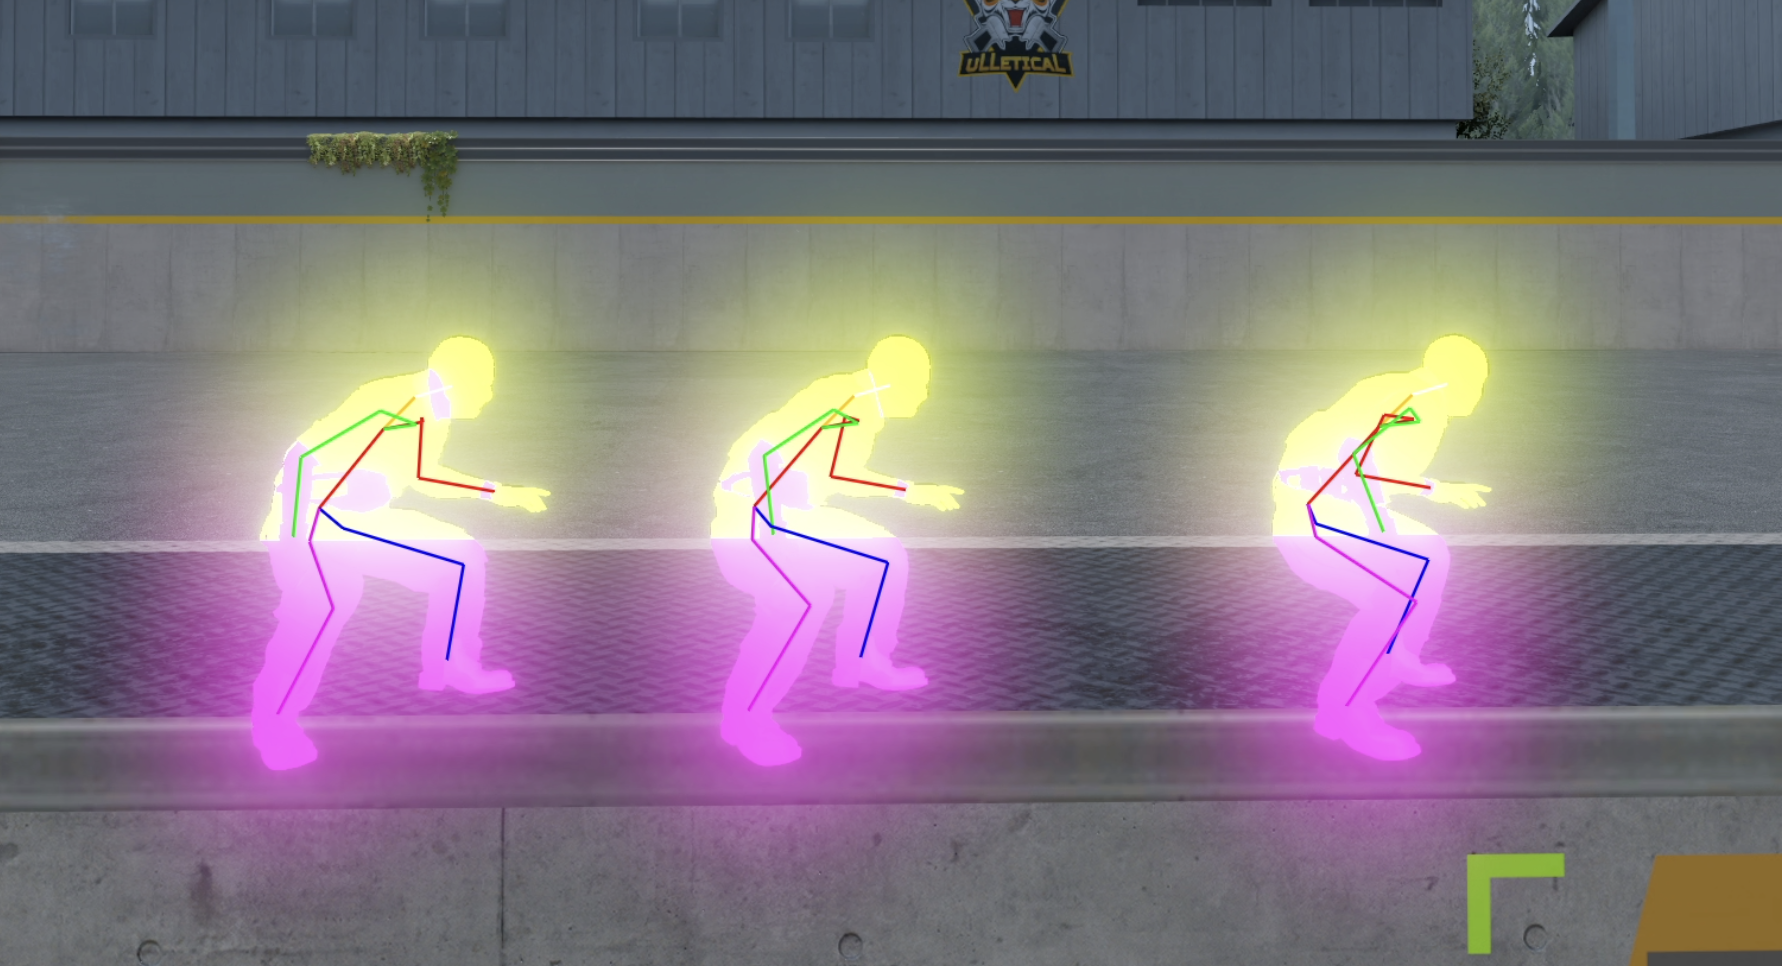
\includegraphics[width=0.33\textwidth,height=0.23\textheight]{images/chams/Screenshot 2025-04-28 at 03.22.41.png}
\end{figure}


\section{Anti-Aim: Misleading Enemy Targeting Systems}

Anti-Aim is a cheat technique designed to manipulate the visible orientation of a player’s model in order to confuse enemy aimbots and reduce the likelihood of being hit in combat. Rather than improving offensive capabilities like an aimbot or triggerbot, Anti-Aim provides a defensive advantage by making it significantly harder for both human players and automated cheats to land accurate shots.

\subsection{What Is Anti-Aim?}

In \textit{Counter-Strike 2}, a player's view direction is broadcast to the server and other clients to render the model's orientation. Normally, this direction reflects where the player is actually looking and aiming. Anti-Aim breaks this consistency by desynchronizing the player's real viewing direction from the one seen by others. As a result, opponents and external cheats perceive the cheater as facing in the wrong direction, leading them to aim at incorrect hitboxes.

This desynchronization creates an illusion where, for example, the cheater may be looking forward from their own perspective, but appear to be looking sideways or even backwards to others. Since many cheats rely on model orientation to predict aim points, this strategy effectively disrupts their logic.

\subsection{Types of Anti-Aim}

There are several ways Anti-Aim can be implemented, each with different goals such as stealth, aggressiveness, or maximum desync:

\begin{itemize}
    \item \textbf{Fake Yaw (Yaw Desync):} The player's view direction (yaw angle) is faked to appear offset from their real direction. This is the most common and effective form of Anti-Aim.
    
    \item \textbf{Pitch Exploits:} Sends pitch values that are outside the game's allowed viewing range (e.g., looking completely up or down), which causes visual glitches in the player model. This can result in the head being rendered inside the chest or legs, making headshots harder.
    
    \item \textbf{Yaw Jitter:} Rapidly switches between multiple fake yaw angles, making the model “shake” or spin unpredictably. While easy to spot visually, this is highly effective against poorly written aimbots.
    
    \item \textbf{Spinbot:} Continuously rotates the model in a full 360° loop at high speed. This guarantees total desync but is highly obvious and generally used in rage hacking contexts rather than legit cheating.
    
    \item \textbf{Static Desync:} Applies a fixed yaw offset to the model, making the cheater appear to always be looking in a different direction. This is more subtle and used in “legit” cheating configurations.
\end{itemize}

\subsection{Lower Body Yaw (LBY) and the LBY Breaker}

In older Source-based games like CS:GO, the engine separated the upper and lower body yaw (LBY) values for animation purposes. LBY would only update under specific conditions, such as when a player stopped moving. Exploiting this timing, cheaters could delay the LBY update and create a temporary desynchronization window between the real view angles and the visible model. This method was known as the \textbf{LBY Breaker}.

While CS2’s Source 2 engine has changed animation handling, similar concepts still apply. Some anti-aim techniques attempt to delay animation state updates or force inconsistent transitions to create fake angles, although LBY is no longer exposed in the same way. Nonetheless, the idea of exploiting animation update delays remains an active area in cheat development.

\subsection{Benefits for the Cheater}

Anti-Aim provides several key advantages:

\begin{itemize}
    \item \textbf{Aimbot Evasion:} Many aimbots target the visible model's head or chest hitbox based on predicted angles. Anti-Aim misaligns these predictions, causing the aimbot to miss entirely.
    
    \item \textbf{Confusing Human Opponents:} Players may struggle to read movement or pre-aim accurately when the enemy model behaves unpredictably or appears to be looking away.
    
    \item \textbf{Reduced Headshot Risk:} By forcing the head into glitched positions (e.g., inside the torso), it becomes harder to land critical hits, especially for players relying on flick shots or crosshair placement.
    
    \item \textbf{Overwatch Safety:} When configured subtly, Anti-Aim can provide these benefits without looking suspicious in demos, reducing the risk of bans from human reviewers.
\end{itemize}

\subsection{Importance in Modern Cheats}

Anti-Aim has become one of the most essential components in competitive cheat configurations, especially in cheat-vs-cheat environments (e.g., HvH—Hack vs. Hack matches). In such scenarios, defensive capabilities are as important as offensive ones, and the ability to evade incoming fire becomes a major strategic advantage.

Furthermore, as anti-cheat systems become more advanced in detecting aimbots and wallhacks, subtle and effective Anti-Aim techniques provide cheaters with a low-profile method to gain survivability without triggering automated bans.






\newpage
\newpage
\newpage
\newpage





 \chapter{Synthesis and Closing Thoughts}

\section*{Synthesis}

This thesis has presented a comprehensive and technically rigorous investigation into cheating within online multiplayer games, using Counter-Strike 2 as a central case study to illustrate both system vulnerabilities and defensive strategies. Beginning with the anthropological foundations of human competition and tracing the evolution of computing and digital interaction, we have demonstrated how cheating practices have co-evolved with the complexity of the platforms they target.

Our analysis addressed not only the broader social and economic impacts of cheating, but also its technical foundations. We examined core mechanisms such as code injection, memory traversal, function hooking, and internal rendering manipulation. These elements collectively reveal how cheats can persist within protected environments and evade conventional detection.

\section*{Practical Contributions}

A primary contribution of this work is the design and implementation of a complete cheat for Counter-Strike 2, developed as a modular and extensible framework. The cheat includes several advanced features:

\begin{itemize}
  \item Engine-level chams and material injection
  \item Entity list traversal and skeletal rendering (bone ESP)
  \item Automated targeting (aimbot) with smoothing and stealth logic
  \item Anti-aim systems including LBY breaking and view desynchronization
  \item Hooking of rendering and input functions using trampolines and MinHook
\end{itemize}

The full source code is publicly available through the accompanying GitHub repository, supported by technical documentation and maintainable implementation practices. It serves as a practical reference for understanding memory manipulation, data tracing, and engine interfacing techniques used in modern game exploitation.

\section*{Final Reflections}

The objective of this research is not to promote cheating, but to expose and analyze its technical underpinnings and broader implications. By making our methodology and tooling accessible, we seek to foster a clearer understanding of how cheats function, how anti-cheat mechanisms respond, and where current approaches fall short. This thesis has shown that cheating reflects systemic design flaws, economic motivations, and a lack of transparency in the gaming ecosystem.

Relying on secrecy for security is no longer effective. Instead, we advocate for open, adversarially-informed development practices where vulnerabilities are studied, documented, and mitigated through shared expertise. The tools and insights provided here aim to support this approach, equipping both researchers and developers to engage critically with the realities of game security.

\begin{tcolorbox}[colback=gray!10, colframe=white, boxrule=0pt, sharp corners]
A defining strength of this work is that it offers both an \emph{offensive} and \emph{defensive} perspective. By dissecting the technical foundation of cheating, we not only expose the methods used to exploit games but also identify the critical points where defense can be reinforced. This dual approach allows for a more holistic understanding of the adversarial dynamics in competitive gaming and provides actionable insight for both cheat developers and anti-cheat system architects.
\end{tcolorbox}

\section*{Future Work}

This project is intended as a foundation for further exploration and development. Several potential improvements and research directions include:

\begin{itemize}
  \item \textbf{Automated Offset Resolution:} Replacing hardcoded offsets with a runtime schema manager that parses Valve's binary schema system. This would allow for dynamic extraction of networked variables and entity layouts, improving resilience to game updates.

  \item \textbf{String Obfuscation and Security:} Enhancing protection against static analysis by encrypting string literals using compile-time encryption libraries such as \texttt{xorstr} or similar approaches.

  \item \textbf{Cross-Engine Generalization:} Expanding the framework to support other Source 2-based titles through adaptable hooking logic and modular rendering components.

  \item \textbf{Instrumentation and Defensive Testing:} Repurposing the cheat framework as a controlled testbed for evaluating anti-cheat detection under realistic attack scenarios, using instrumented hooks and traceable payloads.
\end{itemize}

Each of these directions strengthens the project as a reference for both offensive and defensive research. We encourage the community to expand, refine, and critically evaluate this work in the interest of better understanding the evolving landscape of digital game security.

This framework remains open by design, providing a transparent and extensible platform for those who wish to study, adapt, or confront the technical and ethical challenges embedded in competitive multiplayer environments.
 \chapter*{Project Timeline (Gantt Chart)}
\addcontentsline{toc}{chapter}{Project Timeline (Gantt Chart)}
\markboth{Project Timeline (Gantt Chart)}{}

% ---------- GANTT CHART ----------
\begin{landscape}
  \scriptsize
  \vspace*{-3.3cm}
  \hspace*{-2.35cm}
  \begin{ganttchart}[
    x unit=0.135cm,
    y unit title=0.83cm,
    y unit chart=0.83cm,
    time slot format=isodate-yearmonth,
    vgrid,
    title/.append style={draw=none, fill=titlepurple},
    title label font=\sffamily\bfseries\color{white},
    title label node/.append style={below=-1.6ex},
    title height=1,
    bar/.append style={draw=none, fill=barpurple},
    bar height=0.55,
    bar label font=\scriptsize\color{black!85},
    bar incomplete/.append style={fill=barprogress},
    group/.append style={fill=groupviolet!80},
    group incomplete/.append style={fill=groupviolet!50},
    group right shift=0,
    group top shift=.5,
    group height=.25,
    group peaks height=.15,
  ]{2025-01}{2025-06-30}  
  
\gantttitlecalendar{month=shortname} \\

% --- Investigación --- (5 commits)
\ganttgroup{Initial Research (5 commits)}{2025-01-01}{2025-01-31} \\
\ganttbar{Cheat ecosystem overview}{2025-01-01}{2025-01-20} \\
\ganttbar{Forum analysis (UC, GH)}{2025-01-10}{2025-01-30} \\
\ganttbar{Injection methods \& loaders}{2025-01-15}{2025-01-31} \\

% --- Infraestructura y estructura inicial --- (12 commits)
\ganttgroup{Setup \& Base Code (12 commits)}{2025-01-26}{2025-02-15} \\
\ganttbar{Initial commit \& debugging helpers}{2025-01-26}{2025-01-30} \\
\ganttbar{Pattern scanning, interfaces}{2025-01-28}{2025-02-05} \\
\ganttbar{Entity manager \& player classes}{2025-01-29}{2025-02-12} \\

% --- Desarrollo: Visuales y Aimbot --- (26 commits)
\ganttgroup{Cheat Core Development (26 commits)}{2025-02-13}{2025-04-15} \\
\ganttbar{Aimbot (simple to refined)}{2025-02-14}{2025-03-22} \\
\ganttbar{Player \& weapon chams}{2025-03-12}{2025-03-29} \\
\ganttbar{Anti-aim \& visuals logic}{2025-03-31}{2025-04-23} \\
\ganttbar{Pattern scanning \& VMT hooks}{2025-03-22}{2025-04-10} \\

% --- Menú y configuración --- (7 commits)
\ganttgroup{UI \& UX Polish (7 commits)}{2025-03-24}{2025-04-15} \\
\ganttbar{Menu system \& ImGui}{2025-03-24}{2025-03-30} \\

% --- Integración de funcionalidades avanzadas --- (5 commits)
\ganttgroup{Advanced Features (5 commits)}{2025-04-21}{2025-05-03} \\
\ganttbar{Chams invisibles + walls}{2025-04-21}{2025-05-03} \\
\ganttbar{Aimbot smoothing \& humanizer}{2025-04-15}{2025-05-02} \\

% --- Evaluación & VAC Testing --- (3 commits)
\ganttgroup{Evasion \& Testing (3 commits)}{2025-05-01}{2025-06-15} \\
\ganttbar{VAC behavior analysis}{2025-05-01}{2025-06-15} \\

% --- Tesis --- (10 commits)
\ganttgroup{Thesis Writing \& Diagrams (10 commits)}{2025-04-10}{2025-06-30} \\
\ganttbar{Figures \& TikZ diagrams}{2025-04-10}{2025-06-10} \\

\end{ganttchart}
\end{landscape}





%----------
%	BIBLIOGRAPHY
%----------
\clearpage
\addcontentsline{toc}{chapter}{Bibliography}
\printbibliography

\end{document}
